%%% Local Variables:
%%% mode: latex
%%% TeX-master: t
%%% End:

\documentclass[doctor]{ucasthesis}
%\documentclass[master]{ucasthesis}
%\documentclass[doctor]{ucasthesis}
% \documentclass[%
%   master|doctor, % mandatory option
%   secret,
%   arialtoc,arialtitle]{ucasthesis}

% 所有其他可能用到的包都统一放到这里了,可以根据自己的实际添加或者删除。
\usepackage{ucastils}

% 你可以在这里修改配置文件中的定义,导言区可以使用中文。
% \def\myname{朝鲁}

\begin{document}

% 定义所有的eps文件在 figures 子目录下
\graphicspath{{figures/}}

%%% 封面部分
\frontmatter

%%% Local Variables:
%%% mode: latex
%%% TeX-master: t
%%% End:
\secretcontent{绝密}

\ctitle{面向数据中心服务质量的可编程体系结构}
\makeatletter
\makeatother
\cdegree{工学博士}
\cdepartment[计算所]{中国科学院计算技术研究所}
\cmajor{计算机科学与技术}  %写一级学科名称
\cauthor{马久跃}
\csupervisor{孙凝晖\hspace{1em}研究员}
\csupervisorplace{中国科学院计算技术研究所}

% 日期自动生成,如果你要自己写就改这个cdate
% \cdate{\CJKdigits{\the\year}年\CJKnumber{\the\month}月}

\etitle{Programmable Architecture for Quality-of-Service in Datacenters }
\edegree{Doctor of Philosophy}
\eauthor{Ma Jiuyue}
\edepartment{Institute of Computing Technology, Chinese Academy of Sciences}
\emajor{Computer Science and Technology}   %写一级学科名称
\esupervisor{Sun Ninghui}

% 这个日期也会自动生成,你要改么?
% \edate{December, 2005}

% 中英文摘要和关键字
\begin{cabstract}
  当前数据中心正面临着提高资源利用率与保障应用服务质量的挑战。
  负载融合是提高服务器利用率的主要方式,
  将不同用户的应用部署在同一台服务器,通过资源共享的方式能够提高资源利用率。
  但当前计算机中无管理的软硬件资源共享所产生的资源竞争,
  会给应用带来不可预测的性能波动。
  为了保障延迟敏感型在线应用的服务质量,数据中心系统会倾向于避免共享,
  使用独占或过量资源预留的方式降低由于共享对在线应用的影响,
  造成了数据中心6\%$\sim$12\%极低的资源利用率。

  硬件不能区分来自不同应用的请求,无法实现应用之间的性能隔离,
  使得共享资源的应用之间产生干扰,是数据中心问题的根源。
  因此,在应用数量众多、需求多样且不断变化的数据中心场景下,
  计算机体系结构需要重新设计,为应用提供区分化服务、良好的性能隔离,
  并具备灵活的资源管理编程接口,实现资源使用的强控制与按需分配,
  才能解决数据中心资源利用率与服务质量冲突的问题。

  本文围绕数据中心资源利用率与应用服务质量冲突的问题,
  在服务质量保障的体系结构支持方向上开展研究,主要的工作和贡献包括:

  1)提出``性能标签''概念,用于实现应用区分。
     基于进程的虚拟地址空间抽象无法满足数据中心多租户应用之间的隔离需求,
     一些硬件隔离技术如EPT、I/O MMU、SR-IOV试图扩展现有的体系结构,
     但它们本质上只在功能层面上实现了隔离,
     与性能相关的部件如共享末级缓存、内存控制器等由于缺少应用信息,
     依然处理于无序共享的状况,无法实现性能隔离。
     本文所提出的性能标签抽象,使用统一标签区分不同应用,
     通过在计算机系统内所有请求标识应用标签,让硬件能够实现应用识别与区分化处理,
     实现性能隔离。

  2)提出通用硬件资源管理方法与架构。
     通过统一的资源管理接口实现不同类型硬件上机制与策略的统一管理,
     使用软件编程的方式根据应用需求对硬件的机制与策略进行调整,
     包括基于``控制平面''的策略可编程和``数据平面'' 的机制可编程,
     以支持数据中心复杂多变的应用场景。

  3)提出本地资源带外管理的方式,实现资源管理与业务逻辑的分离。
     在集中式的资源管理模块中,利用Linux的sysfs机制将``控制平面''和
     ``数据平面''抽象为文件,为管理员提供基于文件的硬件资源编程接口。
     实现本地资源的灵活管理。
     同时提出了``\emph{trigger$\Rightarrow$action}''机制实现硬件资源的实时监控与反馈调节,
     以及不同资源之间的协同管理。

  4)构建资源管理可编程体系结构实验平台,包括基于gem5的模拟器与FPGA原型系统,
     其中模拟器已经在LGPL协议下开源。
     FPGA原型系统验证结果表明,通过性能标签与可编程硬件资源共享管理方法,
     PARD体系结构能够为计算机带来应用区分化服务、性能隔离与资源管理可编程特性,
     同时也不会在系统中引入过大的性能开销与资源开销。
     基于以上这些硬件机制与软件栈及适当的资源管理策略,
     PARD体系结构能够进行高效的资源管理,实现数据中心资源利用率与应用服务质量的平衡。
\end{cabstract}

\ckeywords{数据中心, 体系结构, 服务质量, 可编程}

\begin{eabstract}
  Contemporary data centers confront with challenges in
  managing the trade-offs between resource utilization and
  applications’ quality of services (QoS). 
  Co-locate multiple workloads into a single server can
  achieve high utilization.
  But the unmanaged contention for shared hardware resources,
  as well as shared software resources,
  may cause unpredictable performance variability.
  To guarantee QoS of latency-critical online services,
  data center operators or developers tend to avoid sharing by
  either dedicating resources or exaggerating reservations
  for online services in shared environments,
  which result in lower utilization, only 6\% to 12\%.

  Unable to distinguish different applications and achieve performance isolation,
  resource contention in existing computer architecture is the root cause of
  the data center problem.
  Due to the large amount of applications of diverse demands in data center,
  the computer architecture needs redesign to resolve the problem
  by supporting differentiated services, better performance isolation,
  flexible programming interfaces, strong control, and resource on demand.
  
  Focuses on the trade-off between resource utilization and applications'
  quality of services, this dissertation studies the architecture for quality of service
  in data centers. The main works and contributions include:

  (1) A ``Performance Label'' abstraction is proposed
      for applications distinguish purpose.
      %As the emergence of virtualization and cloud computing technologies,
      The virtual address space abstraction introduced by multi-process
      can not support isolation of multi-tenant.
      Recently, some hardware mechanisms, such as EPT, I/O MMU and SR-IOV,
      are proposed to enhance the existing architecture for better isolation.
      Essentially, these mechanisms only achieve functional isolation,
      which means the performance related resources,
      such as shared last level cache, memory controller, are still unmanaged.
      Contention caused by unmanaged sharing makes performance isolation unpractical.
      By tagging all the requests in computer with a uniformed performance label,
      the shared hardware-resources can support differentiated service
      according to the tagged label,
      which brings the benefit of performance isolation.

  (2) An unified resource management method and architecture is proposed,
      which makes ``control plane'' and ``data plane'' abstractions for
      shared hardware resources.
      It manages all shared hardware resources in a programmable manner through
      control plane based strategy programmable and
      mechanism programmable realized by data plane.
      The programmable characteristic makes it more adapted to the complex
      data center scenario.

  (3) An out-of-band resource management architecture is proposed,
      which separate resource management from business.
      In the per-node centralized resource management module, 
      the ``control planes'' and ``data planes'' are abstract as files
      through sysfs mechanisms provided by the linux-based firmware.
      Data center operator can achieve flexible resource management through 
      this file-based interface.
      A ``\emph{trigger$\Rightarrow$action}'' mechanisms is also provided to implement
      real-time resource monitoring and adjustment, and joint management of different
      hardware resources.

  (4) A prototype of the proposed architecture PARD is proposed,
      including an open-sourced gem5-based simulator and a FPGA prototype.
      The results from FPGA prototype shows that, the PARD architecture brings
      the features of differentiated service, performance isolation,
      and programmable resource management with only little resource overheads.
      With these features, PARD can realize efficient resource management and
      achieve balance of the resources utilization and
      applications' quality of service in data center.



\end{eabstract}

\ekeywords{datacenter, architecture, QoS, programmable}


% 设置 PDF 文档的作者、主题等属性
\makeatletter
\ucas@setup@pdfinfo
\makeatother
\makecover

% 目录
\tableofcontents
% 插图索引
\listoffigures
% 表格索引
\listoftables
% 符号对照表
%\begin{denotation}

\item[HPC] 高性能计算 (High Performance Computing)
\item[cluster] 集群
\item[Itanium] 安腾
\item[SMP] 对称多处理
\item[API] 应用程序编程接口
\item[PI]	聚酰亚胺
\item[MPI]	聚酰亚胺模型化合物,N-苯基邻苯酰亚胺
\item[PBI]	聚苯并咪唑
\item[MPBI]	聚苯并咪唑模型化合物,N-苯基苯并咪唑
\item[PY]	聚吡咙
\item[PMDA-BDA]	均苯四酸二酐与联苯四胺合成的聚吡咙薄膜
\item[$\Delta G$]  	活化自由能~(Activation Free Energy)
\item [$\chi$] 传输系数~(Transmission Coefficient)
\item[$E$] 能量
\item[$m$] 质量
\item[$c$] 光速
\item[$P$] 概率
\item[$T$] 时间
\item[$v$] 速度
\item[劝  学] 君子曰:学不可以已。青,取之于蓝,而青于蓝;冰,水为之,而寒于水。
  木直中绳。(车柔)以为轮,其曲中规。虽有槁暴,不复挺者,(车柔)使之然也。故木
  受绳则直, 金就砺则利,君子博学而日参省乎己,则知明而行无过矣。吾尝终日而思
  矣,  不如须臾之所学也;吾尝(足齐)而望矣,不如登高之博见也。登高而招,臂非加
  长也,  而见者远;  顺风而呼,  声非加疾也,而闻者彰。假舆马者,非利足也,而致
  千里;假舟楫者,非能水也,而绝江河,  君子生非异也,善假于物也。积土成山,风雨
  兴焉;积水成渊,蛟龙生焉;积善成德,而神明自得,圣心备焉。故不积跬步,无以至千
  里;不积小流,无以成江海。骐骥一跃,不能十步;驽马十驾,功在不舍。锲而舍之,朽
  木不折;  锲而不舍,金石可镂。蚓无爪牙之利,筋骨之强,上食埃土,下饮黄泉,用心
  一也。蟹六跪而二螯,非蛇鳝之穴无可寄托者,用心躁也。—— 荀况
\end{denotation}


%%% 正文部分
\mainmatter

%%% Local Variables:
%%% mode: latex
%%% TeX-master: t
%%% End:

\chapter{引言}
\label{chap:intro}

互联网与云计算的发展,越来越多的应用从本地迁移到云端,并涌现出大量新兴的互联网应用,
承载这些应用的数据中心成为了如同电力系统一样的社会基础设施。
与此同时,现代数据中心正在面临着权衡资源利用率与应用服务质量的挑战:
从应用开发者角度,服务质量是第一位的,因为它直接关系到用户体验与其收益,
由于互联网应用负载的波动性,开发人员通常会为自己的应用过量分配资源以满足峰值时的负载需求,
这造成了非常低的服务器利用率,通常只有6\%-12\%;
而对于数据中心运维人员,资源利用率直接反映其运维成本,虽然将不同应用混合部署到同一台服务器,
充分利用空闲时段的服务器资源可以有效提高数据中心利用率,
但多应用混合部署引入的软硬件资源共享会造成应用间无管理的资源竞争,
使得应用性能出现不可预测的波动,进而影响应用的服务质量。
由上可知,如何权衡数据中心资源利用率与应用服务质量是当前数据中心亟待解决的重要问题。

可以从三个角度解决这一问题:
其一是通过上层软件机制实现干扰容忍,在应用层保障服务质量,
如Google提出的Hedged Requests和Tied Requests方案\cite{dean_tail_2013},
通过向多个副本发送请求,并选择最快返回的结果以达到干扰容忍的目的;
R. Kapoor等人在文章\cite{Kapoor:2012:Chronos}中提出了Chronos架构,
以降低数据中心应用的长尾延迟;
另外一些工作\cite{timecard:2013, d2p:2014}尝试记录单个请求延迟在每个环节处理时间,
然后在分布式处理框架中传播,基于这些传播的信息来进行请求的处理与调度。
其二是在作业调度层次,通过profile的方式预测应用混合后的干扰情况,
将相互之间干扰较小的应用部署到同一台服务器\cite{mars_bubble-up:_2011, kambadur_measuring_2012}。
其三是提供一个良好的隔离环境,降低由资源竞争所产生的应用间干扰,
可以在各个层次实现隔离,
如数据中心作业调度层\cite{Hindman:2011:Mesos, Schwarzkopf_omega_2013, borg:2015}、
操作系统\cite{cgroup, lin_gaining_2008, tam_managing_2007, liu_software_2012, Liu:2014:ISCA}、
虚拟化层\cite{Xu:2013:Bobtail:, Xu:2013:SMALL}、
硬件\cite{kasture_ubik:_2014, sanchez_vantage:_2011, sanchez_zcache:_2010, qureshi_utility-based_2006, muralidhara_reducing_2011}等。


其中前两种方案在实施时需要对目标应用具有非常深入的理解:
方案一需要对应用架构与实现细节进行修改,以达到应用层干扰容忍的目的;
方案二虽然无需对应用进行修改,但需要对应用的资源占用以及不同应用之间的干扰状况进行分析,
才能得到最优的调度方案。
当应用数量不多且有条件进行以上所述的分析或修改,通过精细的应用架构设计与调度机制,
可以有效的解决前文所提到的资源利用率与服务质量相冲突的问题。
但在现实数据中心特别是云计算数据中心内,以上假设并不成立。

首先,数据中心内通常会运行大量的应用,
如Google的数据\cite{Reiss_googletrace_2012}表明其数据中心在两个月内累计运行超过2,000,000个应用,
无论是改造这些应用或是对应用之间的干扰行为进行分析都是不可行的。
即使只对部分关键的应用进行改造使其适应干扰环境,
云计算环境下的``吵闹的邻居(Noisy Neighbors)''也会使这些努力的结效果大打折扣。

其次,调度方案无法解决短时运行的干扰应用对其他正常应用带来的影响,特别是随着DevOps的兴起,
由于开发调试与线上部署是不断迭代进行的,调试过程中所引入的短时干扰应用数量大大增加,
Google的数据\cite{Reiss_googletrace_2012}发现大量的小于6分钟的应用都是来自于这些调试应用。
当调度器发现干扰并准备采取调度措施时干扰应用可能已经结束,同时新的干扰应用又开始运行,并带来新的干扰。

对于第三种隔离方案,
单纯软件层次的隔离只能做到较粗粒度的资源管理,实现的效果有限;
同时应用的不同特征造成资源竞争点是分布在整个软件栈中,
因此只能根据实际场景做针对性的优化;
再次,在如此复杂的软件栈中找到真正的资源竞争点需要大量的时间与精力,
这同样不能满足云计算的场景下应用多样与快速部署的需求。
除了软件栈上的共享,混合部署的应用在硬件层次上也存在大量的共享,
如共享末级缓存、内存控制器、I/O等,
上文所提到的这些研究专注于如何在这些共享硬件上提供隔离功能,
但这些研究大都只关注于一种类型的资源,而且是针对特定的场景,
因此缺少灵活的软件编程接口,不能适用于通用的计算场景。

综上可知,
现有的三种方案都不能很好的解决当前云计算数据中心中遇到的资源利用率与服务质量矛盾的问题,
该问题的本质是为应用提供区分化服务,
而如何解决目前计算机系统的软硬件资源的无管理共享状态是实现区分化服务的关键。
现有研究在一定程度上能够解决软件层次的共享管理问题,
但无管理的硬件共享使得该问题并没有被完全解决。
造成这一现状的原因是目前的计算机体系结构在设计时并没有考虑到多应用共享场景,
其指令集抽象不足以将上层应用需求传递到下层硬件,
在不能区分应用需求的前提下很难做到区分化服务。
软件层次已有很多方案可以用于区分不同应用,如操作系统级的进程PID或cgroup,
或更细粒度的应用级标签\cite{timecard:2013,d2p:2014, mesnier_differentiated_2011, thereska_ioflow:_2013}。
硬件层次也需要一种应用需求传递机制,
正如``21st Century Computer Architecture''白皮书中所提出的:

\begin{quotation} 
\emph{\textbf{Better Interfaces for High-Level Information.}
Current ISAs fail to provide an efficient means of capturing software-intent or conveying critical high-level information to the hardware.
For example, they have no way of specifying when a program requires energy efficiency, robust security, or a desired Quality of Service (QoS) level.
Instead, current hardware must try to glean some of this information on its own ......
\textbf{New, higher-level interfaces are needed to encapsulate and convey programmer and compiler knowledge to the hardware,}
resulting in major efficiency gains and valuable new functionality.}\cite{21st_architecture}
\end{quotation}

因此,我们需要为数据中心计算机设计一种新的体系结构,
使其能够从硬件上改变资源的``无管理共享''现状以,
从体系结构上支持应用服务质量保障,
在此基础上实现数据中心资源根据应用动态管理以提高资源利用率。

\begin{figure}[H]
  \centering
  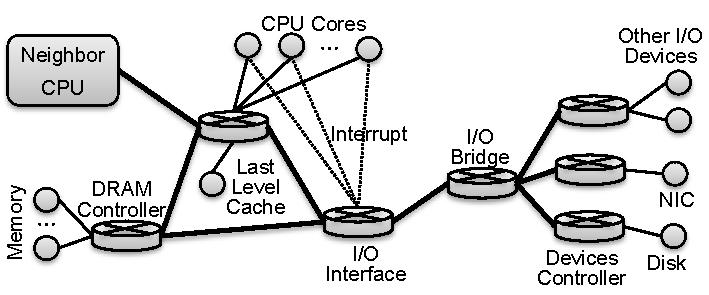
\includegraphics[height=4cm]{intro/computer-as-a-network.pdf}
  \caption[计算机内部本质是一个网络]{
    计算机内部部件之间以数据包(packet)进行通信,比如
    处理器核之间使用基于包的片上网络、
    处理器之间采用基于包的互连协议(如QPI和HT)、
    I/O设备与内存之间则通过PCI-E包进行通信。
    因此,计算机本身即可视为一个网络。}
  \label{fig:computer-as-a-network}
\end{figure}

基于以上需求,
本文提出了一种新体系结构:资源按需管理可编程的体系结构PARD\cite{pard:2015},
使数据中心服务器能够支持区分化服务,通过细粒度的硬件资源管理以及灵活的编程接口,
实现在保障关键应用服务质量的前提下提高服务器资源利用率。
PARD体系结构的核心是基于一个重要的观察:\textbf{计算机内部本质上是一个网络}。
如图\ref{fig:computer-as-a-network}所示,
CPU核、共享缓存、内存控制器、I/O设备等可以被看做是网络节点,它们之间通过包进行通信;
除了处理请求以外,这些``网络节点''与网络中的路由器/交换机具有相似的请求转发功能。
在网络领域,如何实现端到端的服务质量保障已有大量的研究,并已形成标准。
如IETF(Internet Engineering Task Force, 互联网工程任务组)于1998年提出了区分化服务
(Differentiated Services)\cite{DiffServ}的概念,
如今区分化服务已经成为应用最广泛的服务质量保障机制之一;
软件定义网络(SDN)\cite{SDN}的出现,进一步促进了网络领域服务质量保障的发展,其提出的
(1)控制平面与数据平面分离,和(2)集中控制的统一编程接口,
为网络管理带来了极大的灵活性。
本文希望能够将网络领域的区分化服务和软件定义网络的思想应用到计算机内部的网络,
用以解决数据中心当前面临的资源利用率与应用服务质量矛盾。

然而相比在计算机网络,
在体系结构这一``内部网络''中实现区分化服务与软件定义网络的功能需要面临一些额外的挑战:

首先,网络栈是整个网络中产生数据包的唯一位置,因此可以很容易的在其中增加标签机制,
实现网络流的区分。
而在计算机中有大量不同类型的硬件部件都能够向``内部网络''发送请求,
而且这些请求的类型各不相同,
如何为这些来自于不同硬件部件、类型各异的请求增加应用标签是需要解决的第一个挑战。

其次,与网络中交换机或路由器这些只进行存储转发的网络设备不同,
计算机内各个硬件部件通常包含更为复杂的功能,
如:处理器末级缓存需要为请求除完成将请求转发到下层内存控制器外,
还需要决定哪些请求数据缓存在本地,以及替换哪些数据到内存控制器;
内存控制器需要进行复杂的地址映射实现将物理地址映射到DRAM芯片,
同时还需要实现调度策略以提高访存性能;其他一些I/O设备具有更为复杂的功能。
因此如何为这些不同类型的硬件部分提供一个统一的控制平面实现对硬件资源的管理是第二个挑战。

最后,在交换机或路由器中已经为管理员提供了访问和配置其控制平面的固件接口,
而在当前的计算机中并没有类似的的固件接口。
服务器中普遍配置的IPMI/BMC\cite{ipmi}提供了诸如温度监控、电源控制、
BIOS访问等有限的监控与管理功能,利用该模块
如何实现硬件控制平面的管理,以及如何为用户(管理员)提供灵活的访问与编程接口是面临的第三个挑战。

为了解决以上三个挑战,PARD体系结构的核心设计理念可以归结为以下四点:
\textbf{1)标签机制},
通过在请求源(如处理器核或具有DMA功能的I/O设备)增加标签寄存器,使用其记录当前正在使用该部件的应用标签,
发出请求时附带该标签,并随着请求在整个计算机内部传播,实现应用区分;
\textbf{2)可编程控制平面},
为共享硬件资源的控制器增加控制平面,控制平面可根据请求标签查询规则进行区分处理,该规则可通过软件实现可编程;
\textbf{3)节点内统一资源管理},
节点内所有的控制平面通过控制平面网络连接到资源管理模块,提供对控制平面的编程接口,实现所有共享资源的统一管理;
\textbf{4)Trigger$\Rightarrow$Action编程方法},
一种基于动作触发的资源管理策略,实现资源实时监控和调整。

本文后续章节将讨论如何在现有体系结构上扩展以实现标签机制;
通用控制平面的设计以及可编程机制的实现,
并包括末级缓存控制器和内存控制器中控制平面的具体设计;
基于以上两种机制实现无Hypervisor的全硬件支持虚拟化系统,
以及如何实现资源按需分配的区分化服务,并使用模拟器对其效果进行验证。
最后在基于FPGA的原型系统中验证PARD体系结构的效果,
并讨论了原型系统实现过程中的经验与教训。


\section{本文的主要贡献}

本文的论点是:
在应用数量众多、需求多样且不断变化的数据中心场景下,计算机体系结构需要重新设计,
为应用提供区分化服务、良好的性能隔离,并具备灵活的资源管理编程接口,
实现资源使用的强控制与按需分配,
才能解决数据中心资源利用率与服务质量冲突的问题。

本文的主要贡献包括:

% 可在多个层次(虚拟机、进程、线程、API、...)区分应用,实现了NoHyper功能
第一,提出``标签化地址空间(Labeled Address Space)''概念。
正如多进程技术的出现引入了虚拟地址空间抽象,
随着虚拟化、云计算与多租户使用模式的出现,
现有的虚拟地址空间抽象无法满足多租户之间的隔离需求,
一些硬件隔离技术如EPT、I/O MMU、SR-IOV等试图在现有的体系结构下支持隔离需求,
其本质则是在虚拟地址空间外增加一层额外的地址空间,但这些技术只是在功能层面上实现了隔离,
而与性能相关的部件如共享末级缓存、内存控制器等在现有体系结构下并没有实现隔离。
本文提出的标签化地址空间抽象,使用统一标签区分不同应用,
并为计算机系统内所有请求标识应用标签,硬件不再需要通过猜测的方式区分应用,
而是通过标签机制打破目前体系结构中软硬件之间的语言鸿沟,
使得共享的硬件资源能够区分来自不同应用的请求并进行区分处理。
%可在不同层次实现应用区分,如虚拟机、进程、线程或使用API标识的数据/代码段,
%以实现不同粒度的区分化服务。
%以虚拟机粒度为例,通过标签机制以及共享硬件资源内部基于标签的划分机制,
%可将一台计算机划分为多台独立的逻辑域(Logical Domain),
%在每个逻辑域内独立运行操作系统,实现NoHyper\cite{keller_nohype:_2010}的功能。

% 表+Trigger/Action <=> 处理器方案
第二,提出硬件资源共享管理方法,为硬件资源共享提供配置、监控、反馈功能,
实现毫秒(ms)级的性能反馈。
%本文两个重要观点是:资源监控与管理结合,共享资源本地与全局协同管理结合。
实时的监控与反馈是实现细粒度资源管理的重要前提,软件监控方案无法满足实时性的需求,
在硬件上直接实现监控与反馈,提出使用通用的``控制平面''实现硬件资源的配置与监控。
在具体实现上,通过基于表的控制平面实现通用的硬件资源管理接口,
使用基于处理器的数据平面实现硬件请求的灵活控制,
为计算机系统实现硬件资源可管理提供支持。

第三,提出节点内硬件共享资源的协同管理。
控制平面构成了计算机系统内硬件资源管理的基本单元,由于硬件资源之间具有关联性,
需要进行全局统筹管理。
本文通过使用控制面网络将节点内所有的控制平面连接到集中式的资源管理模块,
对硬件共享资源进行协同管理。

以上三点贡献已在PARD的模拟器及FPGA原型系统中实现。
模拟器原型是基于gem5\cite{binkert_gem5_2011}实现的全系统时钟精确模拟器,
增加或修改了大约24,118行C++/Python代码,该模拟器以在LGPL协议下开源
\footnote{PARD-gem5模拟器开源地址https://github.com/fsg-ict/PARD-gem5}。
FPGA原型系统基于MicroBlaze系统在Xilinx VC709开发板实现并完成验证,
系统运行在133MHz频率,包含4个处理器核。
两个原型系统可以作为后续相关研究的参考平台。


\section{论文的组织}

\begin{figure}[htb]
  \centering
  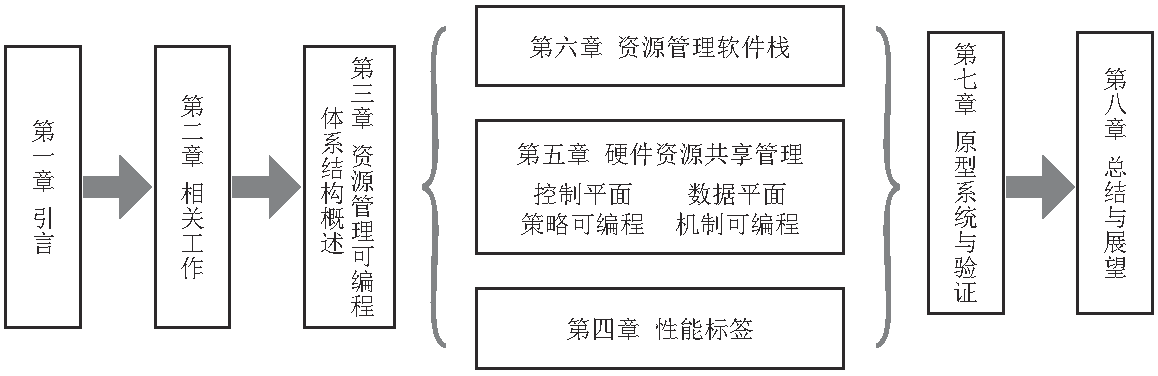
\includegraphics[width=\textwidth]{intro/thesis-structure}
  \caption{本文内容与组织结构}
  \label{fig:thesis-structure}
\end{figure}

本文共分八章,组织结构如图\ref{fig:thesis-structure}所示。

第二章介绍数据中心面临的资源利用率与服务质量冲突问题的挑战,
然后讨论现有数据中心技术的局限性,
并介绍解决该问题的现有研究。

第三章介绍PARD体系结构与关键特性,
并讨论如何利用PARD所提供的特性解决应用服务质量与资源利用率相冲突的问题。

第四章介绍PARD体系结构的基础标签化地址空间,
讨论在现有体系结构下实现标签化地址空间需要解决的关键问题,
并在模拟器上通过标签化地址空间改造,实现无软件支持的全硬件虚拟化功能。

第五章讨论硬件共享资源的管理方法,包括硬件资源的控制平面/数据平面抽象,
同时以共享末级缓存和内存控制器为例,讨论控制平面与数据平面的设计,
并通过模拟的方式验证该方案的有效性。

第六章介绍资源管理模块与资源协同管理相关的内容,包含节点内资源统一管理,
以及如何将PARD集成到现有的数据中心管理系统中(以Mesos\cite{Hindman:2011:Mesos}为例)。

第七章基于前四章的设计给出本文资源管理可编程体系结构的FPGA原型系统实现,
并对原型系统各部分功能的正确性、性能与开销进行评测。

第八章总结全文并介绍未来可能的研究工作。



%%% Local Variables: 
%%% mode: latex
%%% TeX-master: t
%%% End: 

\chapter{相关研究}
\label{chap:related}

互联网应用如电子邮件、搜索、网络购物、社交网络、在线视频、网络地图等, 已经成为人们
生活的一部分。这些应用往往要为上亿用户服务,意味着互联网应用已变成如电力一样的社会
公共服务,而支撑拥有海量用户互联网应用的数据中心也成为如同发电厂一样的社会核心基础
设施。

长尾延迟(Tail Latency)问题在数据中心中受到越来越多的关注,造成长尾延迟的原因有很
多,其中最为重要的原因就是资源共享带来的干扰。
由于没有行之有效的方案对干扰进行控制,目前典型的数据中心都使用隔离的方式来减小干扰,
这一方案虽然有效缓解了长尾延迟,但它也带来了资源利用率过低的问题,
现有商用数据中心的资源利用率普遍只有10\%-30\%左右,造成极大的浪费。
如何解决服务质量与资源利用率的问题是当前业界面临的重大挑战。

本章内容安排如下:首先介绍新计算模式对数据中心的挑战,然后讨论现有数据中心技术的局
限性,即服务质量与资源利率冲突的原因,进而提出一种面向数据中心应用服务质量保障的
体系结构,最后将阐述本文的研究动机,介绍本文的主要贡献和组织结构。

%服务质量(QoS)与资源利用率是数据中心运营时需要考虑的两个重要指标,前者严重影响用户
%体验,而后者直接与数据中心的运营成本相关。然而现有的计算机体系结构并没有为服务质量
%保障提供足够的支持,造成这两个指标在现实状况下存在冲突。为了保障用户体验,在实际系
%统部署时,会更多的考虑服务质量这一指标,造成数据中心的资源利用率严重低下,普遍只有
%10\%-30\%左右。基于这一现状,本文主要讨论如何设计一种高效的数据中心体系结构,使得
%数据中心在保障应用服务质量基础上,达到较高的资源利用率。
%

\section{新计算模式对数据中心的挑战}

\subsection*{计算模式1:以云计算为基础的移动计算}

随着移动设备(平板电脑、智能手机)计算能力不断增强、成本不断降低以及无线通信技术的
快速发展,移动计算时代已经来临。如表\ref{tab:ganter-sales}所示,
Gartner调研数据显示平板电脑和手机(包含智能手机和普通手机)销量不断增加,
与此同时PC销量则不断下降。
而IDC预测到2015年智能手机销量将超过14亿部,占所有个人计算设备(包括PC、平板电脑和智能手机等)69\%的销量份额。

% Gartner关于电脑与移动设备销量的统计 
\begin{table}[htb]
  \centering
  \begin{minipage}[t]{0.9\linewidth}
  \caption[全球个人计算设备市场销量统计]{全球个人计算设备市场销量统计(单位:千部)}
  \label{tab:ganter-sales}
    \begin{tabular*}{\linewidth}{lrrrrr}
      \toprule[1.5pt]
      {\heiti 设备类型} & {\heiti 2012年} & {\heiti 2013年} & {\heiti 2014年} & {\heiti 2015年} & {\heiti 2016年} \\
      \midrule[1pt]
      PC(台式机、笔记本) &   341,273 &   296,131 &   279,000 &   259,000 &   248,000 \\ 
      超级本               &     9,787 &    21,517 &    39,000 &    62,000 &    85,000 \\ 
      平板电脑             &   120,203 &   206,807 &   216,000 &   233,000 &   259,000 \\ 
      手机                 & 1,746,177 & 1,806,964 & 1,838,000 & 1,906,000 & 1,969,000 \\ 
      其它移动设备         &       --- &     2,981 &     6,000 &     9,000 &    11,000 \\
      %总计                 & 2,217,440 & 2,334,400 & 2,378,000 & 2,470,000 & 2,572,000 \\
      \bottomrule[1.5pt]
    \end{tabular*}\\[2pt]
    \footnotesize
    数据来源:Gartner,2012年(http://www.gartner.com/newsroom/id/2610015),
    2013年(http://www.gartner.com-\\/newsroom/id/2791017),
    2014-2016年(http://www.gartner.com/newsroom/id/2954317)
  \end{minipage}
\end{table}

移动计算的快速发展带来新的计算模式:移动设备通过无线通信与运行在云计算平台的各类应
用服务进行交互。据可靠消息,目前一些主要的互联网公司(如Facebook和Baidu等)均表示,
来自移动设备的请求已占到40\%以上,并且仍在快速增长,很快将超过PC。随着4G时代的到来,
这种移动计算模式将成为未来的主流。

快速增长的移动计算需求对云计算平台的核心——数据中心带来了严峻的挑战。这种交互式计算
模式,快速的服务响应时间是衡量服务质量(Quality-of-Service,QoS)的关键指标,是让用
户满意、留住用户的关键。有研究表明,如果服务响应时间增加,公司收入就会减少。
例如,2009年微软在Bing搜索引擎上也开展实验,发现当服务响应时间增加到2000ms时,
每个用户带给企业的收益更是下降了4.3\%。由于该实验对公司产生了负面影响,最终不得不被
终止[8]。Amazon也发现其主页加载时间每增加100ms就会导致销售额下降1\% 。而Google更是
发现当搜索结果返回时间从0.4s增加到0.9s时,广告收入下降了20\%。

\begin{figure}
\begin{minipage}{0.48\textwidth}
  \centering
  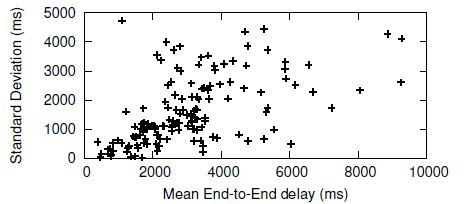
\includegraphics[height=5cm]{intro/end2end-delay}
  \caption[北美移动应用用户感知时延分布]{北美移动应用用户感知时延分布:平均延迟超过2秒且具有很大的波动性}
  \label{fig:end2end-delay}
\end{minipage}\hfill
\begin{minipage}{0.48\textwidth}
  \centering
  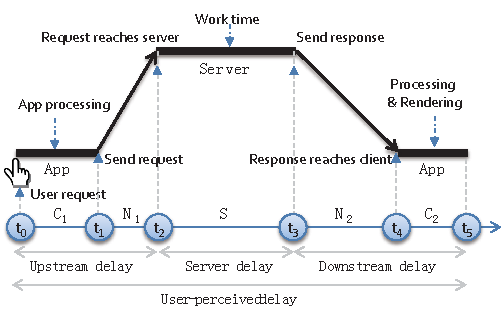
\includegraphics[height=5cm]{intro/interact-apps}
  \caption[一个典型的交互式请求的5个阶段]{一个典型的交互式请求的5个阶段:C1->N1->S->N2->C2 \cite{timecard2013}}
  \label{fig:interact-apps}
\end{minipage}
\end{figure}

移动计算的响应时间仍然存在很大的提升空间。
如图\ref{fig:end2end-delay}所示,微软公司实验数据表明在北美网络环境下,
交互式移动设备的平均时延超过2秒,而且存在较大的波动性。
图\ref{fig:interact-apps}显示典型移动交互式应用的用户请求时延分为5个阶段,
最近研究\cite{timecard2013}表明其中数据中心服务器的处理时延S约为1.2秒,占60\%。
随着4G网络的来临,数据中心将面临更大规模用户数据的处理请求。
因此,如何快速处理和及时响应移动计算请求将成为数据中心设计的核心目标之一。


\subsection*{计算模式2:面向大数据处理的实时计算}

大数据时代的到来使大数据处理架构受到越来越多的关注。2013年底中国计算机学会(CCF)
大数据专家委员会发布的《2014年大数据发展趋势十大预测》 报告中,来自学术界、产业界、
海外、跨界特邀和政府的122位专家们普遍认为,Hadoop/MapReduce框架一统天下的模式将被
打破,而实时流计算、分布式内存计算、图计算框架等将并存。

\begin{figure}[H]
  \centering
  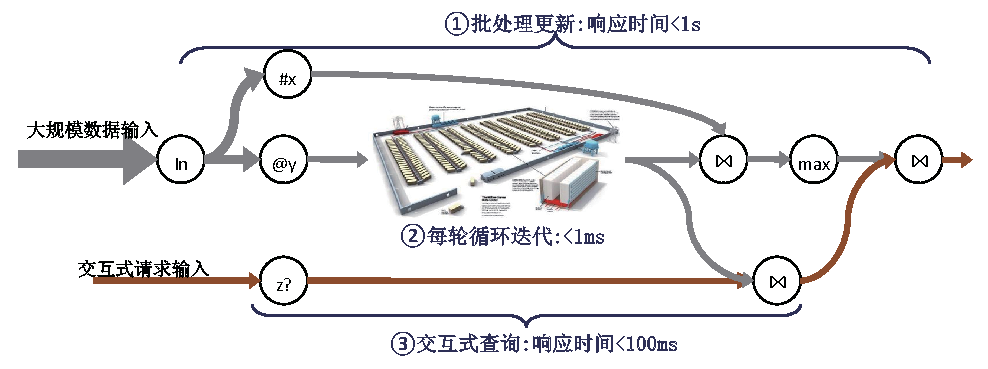
\includegraphics[height=6cm]{intro/batch-apps}
  \caption{典型的3类大数据处理需求以及相应的响应时间要求}
  \label{fig:batch-apps}
\end{figure}


大数据处理对数据中心和处理架构提出新的挑战,图\ref{fig:batch-apps}显示了典型的
大数据处理需求:首先需要支持数据的批处理更新模式(<1s);
其次数据处理会分解为多次迭代计算(<1ms);
再次还要支持实时计算模式,处理多用户的交互式查询请求(<100ms);
而这些处理所需要的数据
存放在同一个数据中心。搜索引擎是一个典型的例子,既需要对大规模网页进行内容处理,
迭代计算页面的pagerank,还需要处理大量用户的关键字查询请求。

尽管大数据处理希望能将各种处理集成在一个处理架构上,然后部署在一个数据中心。但如果
实时计算与企业营收相关,比如搜索引擎、在线购物等在线服务应用,那么正如微软Bing实验
所示,这些面向在线服务应用的实时计算的服务质量就非常关键(以下用“在线应用”
代表“实时计算”)。为了保障在线应用的服务质量,主流互联网企业一般将在线应用与大规模
批处理作业分别部署到不同的数据中心,以减少批处理作业对在线应用的干扰。但由于用户查
询请求数量具有显著的随时间变化的波动性,这种分离作业、单独部署的模式会导致在线应用
数据中心的资源平均利用率很低。如图4所示,Google的两类数据中心CPU利用率相差达2.5倍,
在线应用数据中心资源利用率仍有很大提升空间。


%% 典型的数据中心一般有5~10万台服务器组成,建设与运行维护成本往往高达几十亿人民
%% 币。然而出于保障应用服务质量的原因,现有数据中心只能维持较低的资源利用率,导致大量
%% 资源浪费。因此,本项目总体研究目标为如何设计高效通用数据中心体系结构:“通用”表
%% 示数据中心可同时运行各种不同类型应用;“高效”表示数据中心能在保障延迟敏感应用的服
%% 务质量基础上,达到较高的资源利用率(CPU利用率>60\%)。
%% 
%% 典型的数据中心一般有5~10万台中低端服务器组成,这些服务器通过内部网络互连,一起协同
%% 运行互联网应用为海量用户服务。因为这类数据中心规模很大,往往部署在大型仓库级别的机
%% 房,从应用角度来看就如同一台计算机,因此也被称为
%% “仓库级计算机(Warehouse-Scale Computer)“ \cite{WSC}。
%% 国内外著名的互联网公司往往拥有多个数据中心,服务器数量达到数十万甚
%% 至上百万台。例如,谷歌(Google)的数据中心服务器数量已经超过百万台为全球用户提供
%% 搜索、邮件、地图等服务[2];亚马逊(Amazon)仅EC2就部署了约50万台服务器提供云计算服
%% 务[3];据可靠消息,国内腾讯公司也拥有约30万服务器为用户提供各种互联网服务。
%% 
%% 尽管目前互联网企业的数据中心已经颇具规模,但一个趋势是未来数据中心还将持续发展。一
%% 方面互联网用户数量仍在不断增长,目前全球已有24亿网络用户,但很多机构预测未来全球还
%% 将新增30亿网民融入到互联网[4],这会对数据中心的数量和规模都提出更多需求。另一方面快
%% 速发展的移动终端已超越个人计算机(PC),成为终端计算设备的主流。由于移动设备性能相对
%% 较低、存储容量较小,将计算与存储转移到数据中心的需求也变得越来越强烈。因此数据中心作
%% 为基础设施也会日益重要。


\section{现有数据中心技术的局限性}

通过上述分析可知,移动计算与实时计算均对快速响应用户请求提出了强烈的需求。而当前数
据中心为了保障用户请求的服务质量,不得不通过采用牺牲资源利用率、保留过量资源的方式。
Google的数据中心技术一直处于领先地位,我们以Google为例分析数据中心资源利用率现状。
图\ref{fig:google-util-2006}显示了2006年Google数据中心平均CPU利用率为30\%左右。
但到2013年,虽然Google将数据中心分为了两类,并且批处理数据中心已经能达到75\%的CPU利用率,
但在线应用数据中心仍停留在30\%。
我们对国内企业调研发现,几大主流互联网企业在线应用数据中心CPU利用率一般都低于20\%,
有的甚至低于10\%,仍然存在很大的提升空间。

% Google数据中心利用率 
\begin{figure}
\begin{minipage}{0.57\textwidth}
  \centering
  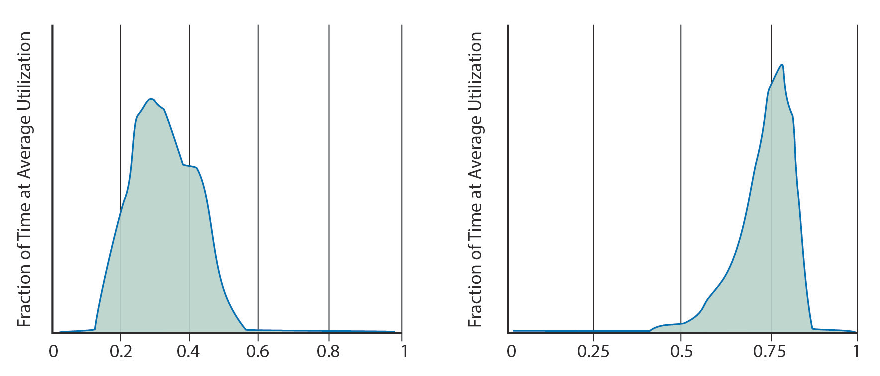
\includegraphics[height=4cm]{intro/google-util-2013}
  \caption[Google数据中心CPU利用率分布(2013年)]
    {Google数据显示2013年1至3月在线应用数据中心CPU利用率平均只有30\%(左图),
     而批处理作业数据中心则能达到75\%的利用率(两个数据中心均为2万台服务器)}
  \label{fig:google-util-2013}
\end{minipage}\hfill
\begin{minipage}{0.39\textwidth}
  \centering
  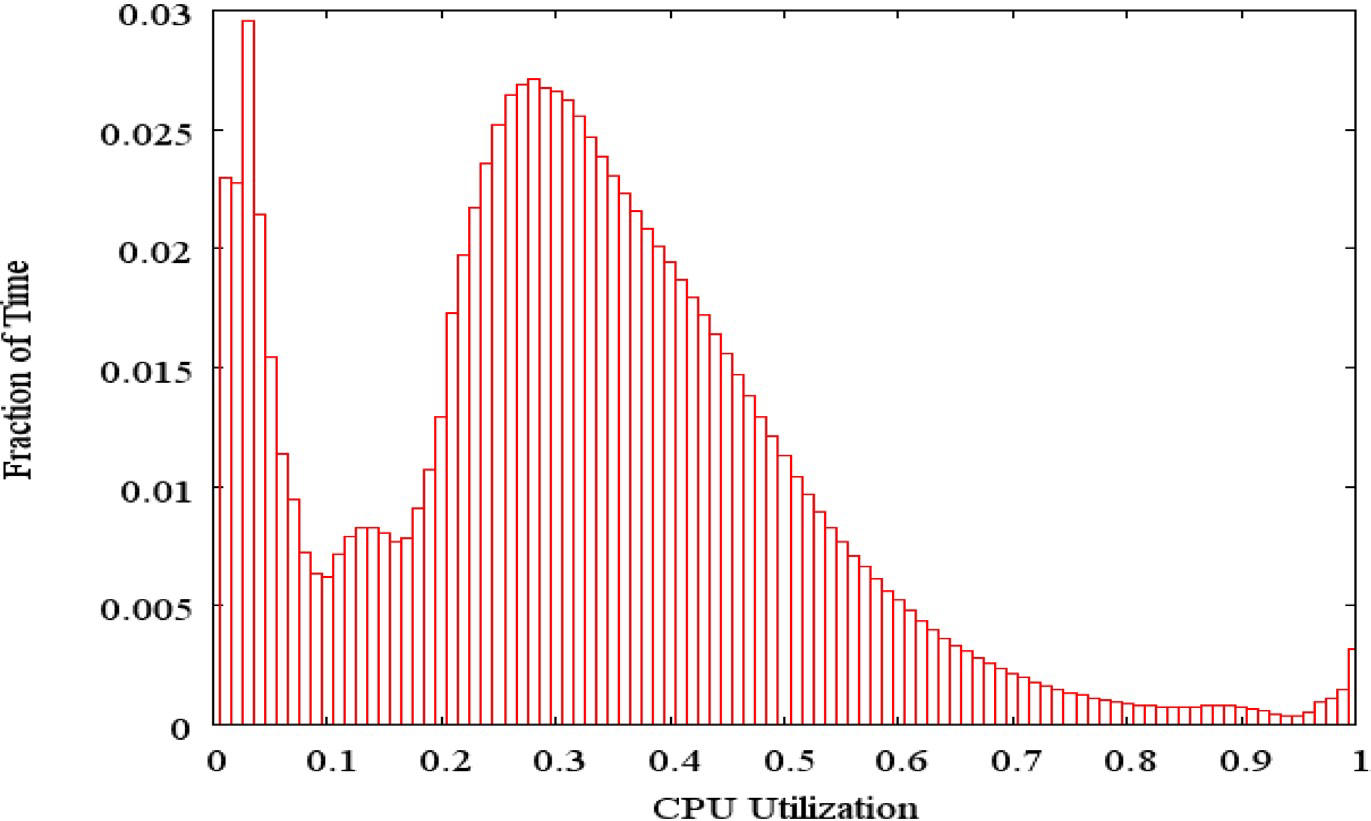
\includegraphics[height=3.5cm]{intro/google-util-2006}
  \caption[Google数据中心CPU利用率分布(2006年)]
    {Google在2006年数据中心(5000台服务器)6个月的CPU利用率分布}
  \label{fig:google-util-2006}
\end{minipage}
\end{figure}

尽管在线数据中心资源利用率只有30\%,但Google已经观察到严峻的长尾延迟现象---最慢的
1\%~10\%请求处理时间远大于所有请求的平均响应时间。
如图6所示,Google某后台服务延迟响应时间平均仅为5~6ms,但是却有相当一部分请求响应时间
超过了100ms[49]。而长尾延迟现象在数据中心环境下会被更进一步放大,因为一个用户请求需要
几百上千台服务器共同完成,只要有一台服务器的处理速度受到干扰,就会导致整个请求的处理
时间增加。Google的Jeff Dean在2012年Berkeley的报告[11]中就指出了长尾现象的严重性,假设
一台机器处理请求的平均响应时间为1ms,有1\%的请求为长尾处理时间会大于1s 
(99th-Percentile)。如果一个请求需要由100个这样的节点一起处理,那么就会出现63\%的请求
响应时间大于1s(如图7所示)。

造成在线应用数据中心资源利用率低和长尾延迟现象的核心原因是现有数据中心技术无法在多
应用混合运行时消除应用间干扰,以实现不同应用之间的性能隔离。
Google的Jeff Dean与Luiz Barroso在2013年2月的《Communication of the ACM》上撰文
“The Tail at Scale”[10]分析确认导致长尾延迟的首要原因就是资源共享,
包括体系结构层次的CPU核、Cache、访存带宽、网络带宽等,而干扰不仅来自应用,
还会来自系统软件层次的后台守护作业、监控作业、共享文件系统等。
Google在分布式架构和软件层次采用了多种缓解长尾延迟的技术,
包括操作系统容器隔离技术[12]、应用优先级管理[13]、备份请求[11]、同步后台管理进程[11]等,
取得了一定的效果,但却无法消除硬件体系结构层次上的应用之间的干扰,
导致仍然会出现图6这样的长尾延迟。

因此,现有数据中心处于“无管理的资源共享”状态,这
导致出现资源利用率与应用服务质量之间的矛盾:
一方面通过多个应用同时在数据中心部署实现资源共享能有效提高资源利用率,
但另一方面多个应用共享资源又会出现相互干扰严重影响应用的服务质量。
因此,目前企业不得不采用预留额外资源以保障延迟敏感的在线应用服务质量,
这导致很低的数据中心利用率。
而且随着多核技术的发展,单个服务器内的资源越来越多,
其上混合部署的应用数目也在不断增加,更会加剧这种矛盾。


\section{本文的研究动机}

现有数据中心技术面临资源利用率与应用服务质量的矛盾,其根本原因是大量数据中心共享资源
属于“无管理共享”状态。要实现高效通用数据中心目标,核心是从硬件上改变资源的“无
管理共享”现状以实现在体系结构上支持应用服务质量保障,在此基础上实现数据中心资源根据应
用动态管理以提高资源利用率。

回顾历史,当前数据中心面临的问题与1990年代的Internet具有相似之处。
当时流媒体、电子商务、电子邮件和FTP等大量网络应用的兴起,它们具有不同的QoS需求。
为了在IP网络中为这些应用提供端到端的服务质量保障,
互联网工程任务组(Internet Engineering Task Force, IETF)于1998年提出了区分化服务
(Differentiated Services)的概念。而如今,区分化服务已经成为应用最广泛的服务质量保障
机制之一。该技术的核心是在IP包头中定义长度为8-bit的区分化服务域,用以表示应用的
服务质量分类标识,因此路由器、交换机等网络设备便可以使用该信息对不同类别的数据包
进行区分处理,以达到区分化服务的目的。
软件定义网络(SDN)的出现,进一步促进了网络领域服务质量保障的发展,
其主要原理可以概括为:(1) 控制平面与数据平面分离;(2)集中控制的统一编程接口。

同时,计算机内部也可以被看做一个网络,如图\ref{fig:computer-as-a-network}所示,
CPU核、共享缓存、内存控制器、I/O设备等可以被看做是网络节点;除了处理请求以外,
这些“网络节点”与网络中的路由器/交换机具有相似的请求转发功能;
而它们之间也通过包进行通信,如:片内通信使用NoC包,片间通信的QPI/HT包,
以及I/O部分使用的PCI-E包。
将网络领域的区分化服务和软件定义网络的思想应用到计算机内部的网络,
用以解决数据中心当前面临的资源利用率与应用服务质量矛盾,是本文的主要研究思路与动机。

与在网络中部署SDN相比,在计算机体系结构“网络”中部署SDN会面临以下三个挑战:

首先,在整个网络栈中EndPoint是唯一的请求来源,因此SDN可以很容易的将标签机制实现在网络栈中;
与之相对的,在计算机体系结构中存在大量的硬件部件都能够发送请求,而这些请求类型又不尽相同,
因此在这样的环境下如何为请求打上标签是一个很大的挑战。

其次,在网络中所有的交换机都执行相同的存储/转发(store-and-forward)操作,但在计算机内部
不同的部件都有不同的功能,而不只是简单的存储/转发,如何为这些不同类型的部件(如末级缓存控制器、
内存控制器、I/O设备等)设计统一的控制面结构是另一个挑战。

最后,在网络交换机中已经包含了一个firmware固件用于访问和配置交换机的控制面,但计算机中却缺少
这样的firmware。现有的IPMI只被用来做有限的监控与管理功能,如对温度、风扇转速和电源控制。
因此,需要在计算机内部提供一种这样的部件实现与其它众多的控制面的通信与管理,并提供一个灵活的
编程接口对这些控制面进行操作。


%本项目总体研究目标是研究新型高效通用数据中心体系结构,能在保障应用服务质量
%的基础上将数据中心计算资源利用率提高到60\%以上。从技术挑战来看,计算机资源管理亟需新的
%具有以下特征的技术架构:
%(1)细粒度共享,有利于提高资源利用率;
%(2)性能隔离,有利于提高应用服务质量;
%(3)快速动态响应,有利于资源按需分配;
%(4)灵活协同配置,有利于协同多种资源配置以适应多种应用场景。


\section{论文的主要工作}

%本研究的目的是通过对真实环境、真实应用的访存行为特征进行更全面细致的分
%析,
%探索服务质量保障的体系结构支持,
%内存系统影响计算机整体性能的更深层次的原因,从而为体系结构、系统软件
%等的设计与优化提供一些建议。

%\begin{description}
% \item[First] \hfill \\
% The first item
% \item[Second] \hfill \\
% The second item
% \item[Third] \hfill \\
% The third etc \ldots
%\end{description}


本研究的目的是在体系结构层次解决数据中心所面临的资源利用率与服务质量相冲突的问题,
论文的主要工作围绕下述三个阶段开展:

\begin{itemize}
 \item 本研究在Xeon E5-v3平台上验证Cache容量划分功能对应用性能隔离带来的作用,
       并提出一种基于反馈模型的缓存自适应分配方法。
 \item 在体系结构内引入标签,实现应用区分,并在各个共享资源对其进行区分处理
 \item 提出一种资源管理可编程体系结构,实现可编程的硬件共享资源的细粒度管理
\end{itemize}


\section{论文的主要贡献}
In this paper, we propose Programmable Architecture for
Resourcing-on-Demand (PARD) that provides a new programming
interface to convey an application’s QoS requirements to the hardware.
PARD supports new functionalities such as fully hardwaresupported
virtualization without software hypervisors and differentiated
service (DiffServ) [60] in data center servers. For instance,
PARD can accurately isolate performance in shared data centers
to improve server utilization without degrading QoS for latencycritical
applications.



\section{论文的组织结构}

本文共分八章,第一章介绍移动计算带来的新计算模式对数据中心的挑战,然后讨论现有
数据中心技术的局限性,并针对现有体系结构提出了新的需求,最后介绍了论文的研究动机、
主要贡献和组织结构。

第二章介绍体系结构领域解决服务质量问题的现有研究,并对比以网络领域的相关内容,
讨论两者相互借鉴的可能性。

第三章对现有体系结构的服务质量支持进行评估,包括软件(cgroup, hyperviso)和硬件
两个层次。

第四章介绍资源管理可编程体系结构的概念与核心思路,并将其映射到现有体系结构,
讨论其可行性。同时应用资源管理可编程体系结构实现全硬件虚拟化,并讨论其关键技术。

第五章讨论模拟器实现,主要从功能设计角度对控制面设计,与资源管理可编程实现,
硬件支持、Trigger-Action机制,模拟的方式验证PARD的有效性。

第六章基于前两章的设计给出本文资源管理可编程体系结构的FPGA原型系统实现,
并对原型系统各部分功能的正确性、性能与开销进行了详细评测。

第七章在数据中心场景下,对本文资源管理可编程体系结构在分布式场景下应用进行讨论。

第八章总结全文并介绍未来可能的研究工作。


处理应用服务质量与资源利用率的问题,在互联网公司、芯片厂商还是学术界都在想办法解决
该问题:互联网公司方面,Baidu的Matrix项目、Google的Borg和Omega、Facebook的mesos系统
都尝试在软件架构层面解决该问题;Intel最新发布的Xeon E5-v3系列芯片,ARM芯片等都对QoS
提供了一定的支持;学术界在软硬件调度、划分方向也有大量工作。但这一问题并没有被解决,
本章首先介绍数据中心应用及其服务质量评价指标,并对现有工作进行总结,并分析其局限性。
同时参考网络领域在解决该问题的方案,

实现高效通用数据中心目标的前提在于保障应用服务质量。类似于系统安全需要所有环节安全
才能保障端到端(End-to-End)的安全,服务质量保障也需要应用全生命周期所有环节的支持。
在数据中心层面,这需要从服务器节点内部、服务器之间通信以及分布式架构多个层次协同工作。
近年来,学术界、工业界在这三个层次都不断努力。例如,近年来流行的Software Defined
Networking(SDN)技术\cite{SDN}目标就是解决数据中心网络通信的管理、共享与性能隔离问题。
Google在分布式架构上采用了超时发送备份请求同步后台管理进程等技术[11]来提高服务质量。
单节点内服务质量保障技术已成为短板。由于体系结构上不支持服务质量保障,而主流的软件
隔离技术能对资源容量隔离起到较好的效果,但无法保障性能隔离,无法保障服务质量。
总的来说,国内外在保障应用服务质量方面的研究包括单节点与分布式环境两个方面。
以下分别从这两个方面介绍相关工作。


应用混合的目标分为两方面:一是提高资源利用率,二是保障关键应用的服务质量。现有的运行时
管理方案[15]–[17]大都通过硬件性能计数器对关键应用的性能进行监控,并在性能发生下降时对非
关键应用进行各种处理,以减小由于资源竞争引起的性能问题。

造成资源利用率的核心问题在于计算机资源处于“无管理共享”状态,因此多个应用共享资源时会发
生竞争与干扰,最终导致关键应用性能不可预测。目前尚无很好的技术方案解决计算机资源“无管理
共享”的问题,以Google为代表的工业界采用将在线服务器与离线服务器分离的方法,通过降低在线
服务器的负载来保障在线应用的服务质量。

学术界在共享资源管理方面从2个维度、4个方面开展研究:软件调度、软件划分、硬件调度、硬件
划分。软件调度是通过操作系统/Hypervisor层次进行进程、线程或虚拟机级别的调度,一般调度粒
度较大,需要上下文切换,时间上也需要几毫秒到几十毫秒,不能满足在线应用的快时响应的需求;
软件划分技术能对Cache容量进行划分,但无法管理访存带宽这类资源,且软件划分技术配置调整开
销较大;硬件调度技术能支持访存请求级别的细粒度调度,但灵活性较多,不能根据不同应用按需管
理;硬件划分技术对Cache容量比较有效,但也无法对带宽等进行管理,而且同样面临灵活性差的问
题。面对诸多问题,斯坦福大学Christos Kozyrakis教授提出应该重新考虑整个计算机架构,从应用
特征、硬件隔离、操作系统、机群调度、高效资源管理硬件等多层次协同设计[18]。

\section{调度方法}
\label{sec:other}

实现高效通用数据中心目标的前提在于保障应用服务质量。类似于系统安全需要所有环节安全才能保障端到端(End-to-End)的安全,服务质量保障也需要应用全生命周期所有环节的支持。在数据中心层面,这需要从服务器节点内部、服务器之间通信以及分布式架构多个层次协同工作。近年来,学术界、工业界在这三个层次都不断努力。例如,近年来流行的Software Defined Networking(SDN)技术[15]目标就是解决数据中心网络通信的管理、共享与性能隔离问题。Google在分布式架构上采用了超时发送备份请求同步后台管理进程等技术[11]来提高服务质量。单节点内服务质量保障技术已成为短板。由于体系结构上不支持服务质量保障,而主流的软件隔离技术能对资源容量隔离起到较好的效果,但无法保障性能隔离,无法保障服务质量。

总的来说,国内外在保障应用服务质量方面的研究包括单节点与分布式环境两个方面。以下分别从这两个方面介绍相关工作。

1.2.1 单机保障服务质量研究

单机保障服务质量相关研究包括软件资源隔离技术、软硬件调度技术、硬件支持等。

软件隔离技术:针对数据中心里多个应用相互干扰的问题,一般采取虚拟化的手段在资源共享的条件下保障资源隔离,如虚拟机技术Xen[18]或Linux Container[17]。

传统虚拟机技术通过将多台虚拟机VM部署到物理机上,每台虚拟机运行一个应用或应用的一个组件,每个应用在自己的操作系统环境中独立运行,减少相互之间干扰。但这些隔离主要是资源的隔离,而无法实现性能隔离。例如为不同应用分配不同的访存带宽。而且使用虚拟机也会带来一定的性能损失[20],增加延迟,带来性能波动。

Linux Container[17]是一种轻量级虚拟化,通过在操作系统层面增添虚拟服务器功能,操作系统内核能够提供多个互相独立的用户态实例。每个用户态实例对于它自己的用户来说都像是一台独立的计算机,有自己独立的网络、文件系统、库函数和系统设置等。操作系统级虚拟化技术的优点是性能开销较小,不需要硬件的特别支持,而且能为用户态实例之间提供一定的隔离性,所以被广泛地应用在虚拟主机服务器环境中。然而,容器虚拟化技术的虚拟对象不是实际的物理资源(处理器、内存和外设),而是从用户角度出发而抽象的操作系统内部资源资,如CPU时间,内存,I/O带宽等,但如图1.5所示,Container技术对性能隔离效果并不理想。事实上,在性能隔离方面也有相关研究, Rice大学的Druschel等人[21]设计了Resource Container系统, 实现了单台物理机上多个应用间的性能隔离和CPU细粒度资源分配机制支持,然而局部隔离并不能保证全局隔离,Druschel 等人又设计了Cluster Container系统[22],以解决应用在集群范围内的隔离问题。但十几年前,单机核数目非常小,如今单节点已经有几十个核,同时运行的应用也增加了一个数量级,出现了很多新的挑战。

页着色(Page Coloring)[33]是一种以软件方式控制内存物理页映射到处理器缓存上的技术,映射到同一缓存块中的物理页对应同一颜色。基于页着色技术可以实现对共享二级缓存的划分(Partition)[36],能缓解应用在共享二级缓存上的干扰。Cho等人[34]使用Page Coloring技术来管理共享缓存。Tam等人[35]在Linux内核上实现了基于页面着色的缓存划分策略。而对于DRAM系统,也可以使用页着色技术对共享DRAM颗粒进行划分[37][39],例如,Liu等人[40]在Linux内核上实现了基于页着色的DRAM颗粒划分。北京大学李晓明教授团队也在这方面做了很多工作[41][42][43],研究利用页着色技术在虚拟环境下对共享Cache进行了划分。页着色技术能缓解一些粗粒度共享资源层次的干扰,但无法解决微体系结构的干扰,比如共享队列等,并且使用不灵活。总结而言,软件隔离技术能对资源容量隔离起到较好的效果,但无法保障性能隔离,无法保障服务质量。

软硬件调度:在多核微体系结构上,由于共享片上和片外资源的竞争会引起跨核应用之间的干扰。Jason Mars和Neil Vachharajani等人提出了竞争感知的轻量级运行时环境CAER[25],能在提高利用率的同时减少由竞争引起的跨核干扰问题。他还和Lingjia Tang等人在文章[24]还介绍了CiPE框架,可以直接用于测量和量化多核结构下应用的跨核干扰敏感度。Jason Mars等人还设计了Bubble-Up[23]机制,通过使用气泡(Bubble)来代表内存子系统的可变压力情况,能准确预测在内存子系统中竞争共享资源而导致的性能下降。Lingjia Tang等人在文章[29]提出了一种动静结合的编译方法ReQos,在确保高优先级应用的服务质量的同时让低优先级应用也可以自适应地执行。ReQoS包含一种由配置文件引导的编译技术,来识别低优先级应用中有争议的代码段。这些调度相关的工作,在具有大规模真实应用的Google“混布”数据中心里,使用该机制能在保证延迟敏感性应用的服务质量的同时,能显著提高50%~90%的资源利用率。但这些工作属于Ad-hoc类型,针对特定场景有效,并没有从根本上解决问题。

以CMU的Onur Mutlu为代表的一些学术界专家在提出了一系列调度算法[44][45][46]以缓解内存控制器的不公平问题,从而提高系统吞吐量以及服务质量。但这些算法是固化的,并不能针对某个应用进行调节,不具有灵活性。

体系结构支持:Ravi Iyer在文章[30]中提出了一种保障CMP体系结构上缓存Qos的管理框架,设计了CQos优先级分类、优先级分配和优先级执行。CQos优先级分类和优先级分配采用的是从用户到开发人员驱动的编译检测和基于流的方法;CQos优先级执行则包括(1)选择高速缓存分配、(2)动静态结合设置分区、(3)异构缓存区域。实验结果表明, CQoS在多线程或多核平台上能提高共享缓存的效率和系统性能。然而,文章[30]并没有详细描述保障CMP体系结构上缓存Qos的具体策略和软硬件支持。所以,Ravi Iyer等人又在文章[31]中实现了一种在CMP平台上保障Qos的内存体系结构,允运行时的动态资源再分配,能在减少低优先级应用性能下降的同时优化高优先级应用的性能。Andrew Herdrich等人[32]证明了用于功耗管理的基于速率(rate-based)的技术能适应于CMP结构上缓存/内存的Qos管理,其基本方法是当正在运行的低优先级任务由于资源争用而干扰了高优先级任务的性能时,就减缓核心的处理速率。通过评估时钟调制和频率缩放这两个速率限制机制,发现时钟调制更适用于缓存/内存Qos管理。

Ravi Iyer在体系结构支持服务质量方面做了一些有价值的工作,但主要集中在内存方面,并没有从整个系统角度去考虑。事实上,我们认为这个方向在未来会越来越重要,值得深入研究。
 
1.2.2 分布式环境保障服务质量

在分布式环境下,影响应用服务质量的因素主要是节点故障与干扰引起的长尾延迟,下面将从这两个方面介绍相关优化技术。

软硬件故障:Jean Dean等人设计MapReduce[26]的初衷是使用由成百上千机器组成的集群来处理超大规模的数据,所以,要求必须MapReduce能很好地处理机器故障。MapReduce采用了任务重新调度或重新执行任务(backup task)的方法来解决节点故障或短暂忙碌。比如,如果一个机器的硬盘出了问题,读取数据的速度从30M/s降低到1M/s, MapReduce框架中发送backup task机制来减少这一类长尾延迟。Backup task机制通常只会占用比正常操作多几个百分点的计算资源,但能显著改善因为故障出现的长尾延迟。不过,类似于TCP重传机制,backup task的有效性会随着负载的提高而削弱。


竞争共享资源引起的干扰:为了缓解干扰引起的长尾延迟现象,Dean等人[10]介绍了Google采用的缓解长尾延迟的技术,包括操作系统容器隔离技术[12]、应用优先级管理[13]、备份请求[11]、同步后台管理进程[11]等。R. Kapoor等人在文章[27]中提出了Chronos架构,以降低数据中心应用的长尾延迟。Chronos基于NIC上应用层数据包头字段的请求划分、应用实例负载均衡和NIC负载均衡模块的加载来消除关键通信路径上的共享资源,如内核和网络协议栈,以减少应用延迟以及相关干扰。

这些研究工作从分布式架构上一定程度上缓解了“划分/聚合”模式应用(如搜索、大数据分析等)的长尾延迟,但对“依赖/串行”模式(在线购物、社交等)应用并不显著。另一方面,随着单个服务器节点的核数目不断增加,甚至未来“片上数据中心”[47]出现,单节点内同时运行的应用也会增加,那么干扰将会越来越严重,仅仅依赖分布式架构以及软件方法将无法保障性能隔离,如何从硬件上支持服务质量保障技术将是一个值得关注与研究的方向。


\section{隔离方法}
\label{sec:multifig}

\section{软件定义网络SDN}
\label{sec:background:sdn}

The Need for a New Network Architecture % [REF] "Software-Defined Networking: The New Norm for Networks" (PDF). White paper. Open Networking Foundation. April 13, 2012. Retrieved August 22, 2013.
The explosion of mobile devices and content, server virtualization, and
advent of cloud services are among the trends driving the networking
industry to reexamine traditional network architectures. Many conventional
networks are hierarchical, built with tiers of Ethernet switches arranged in
a tree structure. This design made sense when client-server computing
was dominant, but such a static architecture is ill-suited to the dynamic
computing and storage needs of today’s enterprise data centers,
campuses, and carrier environments. Some of the key computing trends
driving the need for a new network paradigm include:


\section{本章小结}

从现有技术来看,单节点内服务质量保障技术的不足,导致节点内应用相互干扰严重,某种程
度上成为目前数据中心整体服务质量保障的短板,是成为长尾延迟现象的主要因素之一。同时
这也是一个非常具有挑战的问题,这需要跨层次协同设计。美国计算共同委员会(Computing 
Community Consortium)于2012年5月发布的计算机体系结构共同体白皮书《21世纪计算机体系
结构》中也将单节点内保障服务质量作为未来研究方向之一,其中认为[9]:“管理应用之间的相
互作用也带来了挑战。例如,这些应用如何表达服务质量(QoS)目标并且让底层的硬件、操作
系统以及虚拟层共同工作来保障它们。”



%%% Local Variables: 
%%% mode: latex
%%% TeX-master: t
%%% End: 

\chapter{资源管理可编程体系结构PARD}
\label{chap:pardarch}

本章介绍PARD体系结构的基本架构,
并通过管理员视角介绍PARD体系结构的关键特性,包括:
实现全硬件支持的虚拟化、性能监控与反馈、以及可编程的资源管理机制。
%最后讨论了如何在现有体系结构中扩展以支持PARD的这些关键特性。

\section{PARD体系结构}

PARD是在传统服务器体系结构的基础上进行功能扩展,
实现可管理的硬件资源共享与区分化服务的计算机体系结构实现。
可以从用户、管理员和体系结构三个视角理解PARD体系结构(图\ref{fig:pard-views}):
从用户的视角,PARD是一个可以划分为多个子机器的计算机,每个子机器可以运行独立的操作系统,
不同用户的子机器之间不会存在干扰,用户可根据自己的需求对资源的使用情况进行约定,
如Cache占用、访存带宽等,对子机器的执行性能可预测;
从管理员的视角,PARD是一台具有硬件资源细粒度管理能力的服务器,
通过服务器上配置的资源管理模块(Platform Resource Manager,PRM),
可以监控每个用户对不同硬件资源的使用情况,并可根据需求对资源使用情况进行调整;
从体系结构的视角,PARD将网络的概念引入到计算机体系结构中,
在体系结构内实现了应用区分,为共享硬件部件增加可编程能力,并实现计算机内统一的资源管理。

\begin{figure}[t]
  \centering
  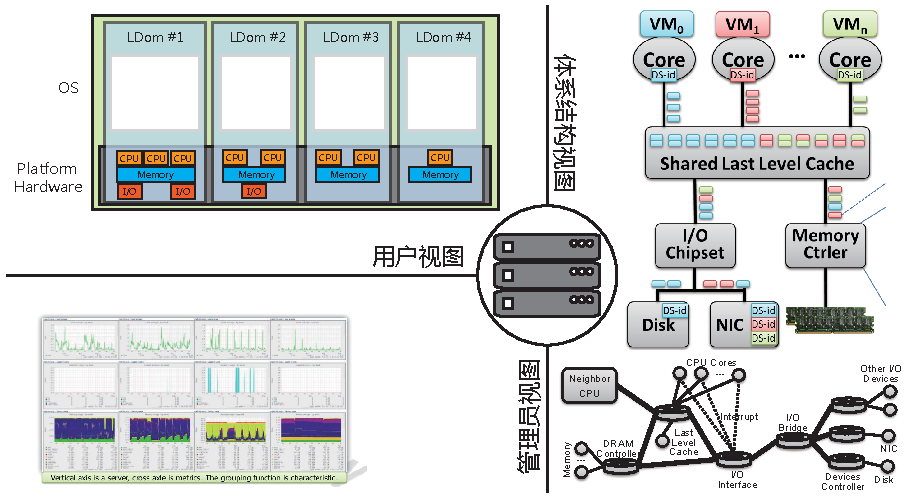
\includegraphics[width=\textwidth]{arch/pard-views.pdf}
  \caption{PARD体系结构}
  \label{fig:pard-views}
\end{figure}

在多应用混合这种共享场景中,隔离性和可管理性是服务器体系结构设计时需要考虑的重要问题。
\textbf{隔离性}是指要让运行在共享环境中的应用无法感知到其它应用的存在,
就像它正在运行在独占的计算机中一样,这其中包含两个层次的概念:
一是资源隔离,即应用独占分配给它的资源;
二是性能隔离,使得应用的性能不会被其它应用所干扰。
现有的软件方案(如多进程、容器、虚拟化)或硬件方案(如LPAR、Logic Domain)
可以很容易实现不同级别的资源隔离,但它们都无法完全实现性能隔离。
首先,在操作系统或虚拟化的软件栈的各个层次中都存在不同程度的共享,
这些共享点在一些特定的场景会产生干扰;
而即使是硬件隔离方案,虽然消除了软件层次的干扰,但在共享硬件资源上的干扰依然存在。
硬件层次的隔离没有发挥应有的效果主要是由于目前的体系结构中并不能识别不同的应用。
\textbf{可管理性}是能够对应用占用的资源进行监控与管理。
由于不同的应用或应用运行的不同阶段,其对资源的需求是不同且不断变化的,
如何获取应用资源需求的变化,以及如何根据这些变化对资源的分配进行调整。

PARD选择了硬件隔离方案,为用户提供逻辑域的抽象以实现资源隔离,
通过使用标签的方式将服务器划分为不同的地址空间,以实现性能隔离;
在各个硬件部件上增加了控制平面与可编程可能,实现共享资源管理;
通过节点内全局的资源管理,实现资源按需分配与动态调整。

\subsection{PARD示例:用户与管理员视角}

本节将从用户和管理员的视角,给出PARD在共享数据中心场景中的应用,
介绍PARD的关键特性,以及如何使用PARD解决硬件资源共享带来的干扰问题,
图\ref{fig:pard-example}为该示例的流程。

1. 在T1和T3时间,用户A和用户B分别希望在服务器上运行应用,
他们将自己的资源需求发送到管理员,管理员在收到请求后,
决定将两个用户的应用运行在同一台PARD服务器上。
在真实的场景中,用户与管理员并不会直接操作服务器,
而是通过如mesos\cite{}、OpenStack\cite{}等集群管理系统使用服务器资源。
这里为了简化描述,将集群管理系统这一层移除,让用户与管理员直接操作服务器。

2. 管理员在T2和T4时刻分别处理用户的请求,并通过服务器的PRM接口将资源需求发送到服务器,
交由运行在PRM中的固件对请求进行处理,并分配资源。
以用户B为例,PRM首先为其创建一个逻辑域(LDom),并根据需要为其分配资源,
该逻辑域的编号为“1”(后续使用LDom1表示该逻辑域)。
由于LDom1是一个普通优先级的应用,PRM为其分配了默认的资源使用策略:
与其它逻辑域共享末级缓存、内存、I/O等硬件资源。
在将这些策略编程到各个设备的控制平面后,PRM完成对LDom1的初始化,并在其中启动操作系统。

3. 在T5时刻,用户C希望执行一个高优先级、延迟敏感型的应用,并通过管理员将请求发送到PRM。
在T6时刻,PRM创建了逻辑域LDom2,并为其分配了高优先级的资源分配策略,
在完成LDom2的初始化后,将用户C的应用部署在该逻辑域中。

4. 在T7和T8时刻,更多的用户将资源需求提交到服务器,服务器的资源利用率持续上升。

5. 在T9时刻,由于服务器内运行的应用在共享末级缓存中产生了严重的干扰,
用户C应用的缓存缺失率急剧上升(>30\%)。
在传统的服务器中,如此高的缓存缺失率会造成应用性能的严重下降,
响应时间出现明显的长尾。而在PARD服务器中,用户C的缓存缺失率上升达到30\%时,
末级缓存会向PRM发送该事件的事件通知,运行在PRM中的固件检测到该事件通知,
执行该事件对应的动作脚本,实现资源的重新分配。
在本例中,该事件的动作脚本将为用户C分配更多的末级缓存容量,以缓解其缺失率更高的问题。
通过以上动作,使得在PARD服务器中用户C应用的性能(响应时间)没有受到严重的影响。

\begin{figure}[t]
  \centering
  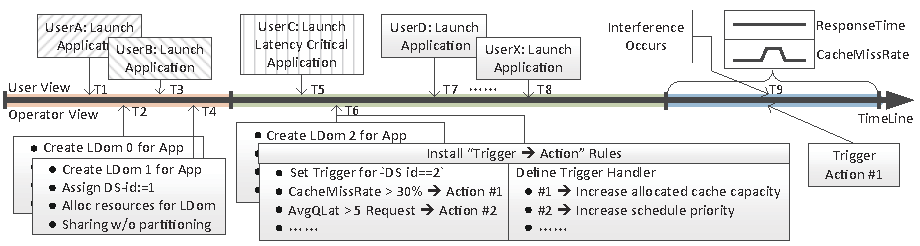
\includegraphics{arch/pard-example.pdf}
  \caption{PARD示例}
  \label{fig:pard-example}
\end{figure}


\subsection{体系结构视角}

计算机是一个网络,


\subsection{PARD关键特性}

在上节中,本文通过实例对PARD体系结构的关键特性做了描述,
本节将对这些特性进行总结(如表\cite{}所示),并简要介绍其实现原理。

% 关键技术点
\textbf{标签化地址空间}\ 传统计算机架构使用单一地址空间,虽然虚拟内存与扩展页表机制
为不同的应用或虚拟机分配独立的逻辑地址空间,但它们还是共享一个物理地址空间。
这种单一地址空间的设计,使得共享的硬件部件不能识别出来自不同应用的请求,
造成应用之间由于竞争硬件资源而产生相互之间的干扰,影响应用的性能。
标签化地址空间是指让计算内所有的请求都携带应用的标签信息,
让共享的硬件部件能够识别出来自不同应用的请求,以实现应用之间的区分化服务。
标签粒度有多种选择,可根据实际的应用需求使用虚拟机、容器、进程、线程
或是一个代码段作为标签。
在现有体系结构上实现标签化地址空间主要需要三个方面的修改:
%第一方面,加寄存器
首先,需要在请求的发起端(如处理器核或带有DMA的I/O设备)增加一个标签寄存器,
用以记录当前应用的标签,并在请求产生后将标签附加到请求上;
%扩展数据通路,传播标签
之后需要在计算机内的数据通路中传播请求的标签,
这些数据通路包括片上网络、处理器之间的互连总线(如QPI或HT)、
I/O总线(如PCI-E)等,目前的体系结构实现中这些总线都使用基于包的总线协议,
因此可以很容易的扩展请求包,将应用标签附加到总线上;
%修改不支持标签传播的硬件,如Cache
第三,修改数据通路上一些不能支持应用标签传播的硬件部件,
使其能够将应用标签正确的传播到下一级通路,
以共享末级缓存为例,对于使用WriteBack策略的共享末级缓存,
由于缓存替换所引起的写回操作,被替换的数据与造成替换的请求并非属于同一个应用,
因此需要在缓存的TagArrary中记录数据所属的应用标签,
在发生缓存替换时,被写回的数据需要附加上TagArray中记录的应用标签,
而不是引起缓存替换的请求所附带的应用标签。
本文将在第\ref{chap:labeladdrspace}章详细讨论在现有体系结构下如何实现标签化地址空间。


%简单说就是加控制平面做管理,数据平面加处理器实现可编程
\textbf{可管理的硬件资源共享}\ 在通过标签化地址空间实现应用区分后,需要对硬件资源的共享访问进行管理。
在现有的体系结构实现下,已经存在一些硬件支持共享管理,
如处理器可通过时间片调度的方式对共享行为进行管理,
Intel在其最新的Xeon E5v3系列处理器中增加了对Cache的容量划分的支持\cite{intel-cat},
可以通过其增加的配置寄存器管理不同应用允许使用的缓存容量。
但除些之外,其它一些重要的共享硬件资源,如内存控制器、I/O等,并不支持对应用共享访问进行管理。
例如,现有的体系结构实现下,无法实现调整某一应用所能够使用的访存带宽、访存优先级或I/O带宽等。
本文提出一种硬件资源共享管理的方法,让计算机内所有重要的共享硬件都支持共享管理,
同时为上层管理员提供一个统一的管理接口。
该方法来源于软件定义网络(SDN)中所提出的控制平面与数据平面的概念,
在SDN中,通过将网络设备划分为控制平面与数据平面,使用控制平面进行管理,数据平面进行转发,
以实现灵活的网络管理。
由于计算机可以被看作是一个网络,与SDN的方法类似,
通过修改硬件的“数据平面”,为其增加可编程能力,实现对应用进行区分处理的功能,
并为硬件部件中增加控制平面,为上层提供统一的资源管理接口,
管理数据平面可编程机制所提供的共享管理特性。
其中控制平面使用基于表的方式,为上层提供管理接口,而数据平面中使用可编程处理器的方式为硬件提供灵活的管理功能,
本文第\ref{chap:hwresman}章将对PARD所提供的硬件资源共享管理机制进行详细讨论。


% 资源监控 + Trigger=>Action反馈 + 全局资源调节
\textbf{资源按需分配}\ 集中式的资源监控,资源全局调节,Trigger=>Action的反馈调节机制。


本文第\ref{chap:hwresman}章将对资源监控与反馈调节机制进行分析,资源的全局管理将在第\ref{chap:global}章进行讨论。


\section{PARD服务器操作}

本节介绍PARD服务器基本操作流程,包括逻辑域创建、资源调整、以及性能监控与反馈。
首先我们定义一台PARD服务器,本节后续内容将以该PARD服务器为实例,
其主要配置如下:

8个处理器核,每个处理器核中包含私有L1 I-Cache和D-Cache;

共享16MB的L2 Cache,使用24路组相联映射;

共享内存控制器,内存容量为8GB;

共享I/O子系统,包含8个SATA硬盘和4个千兆以太网卡。

该服务器共享硬件资源(处理器核、L2 Cache、内存控制器、I/O子系统)都实现了
上节所述的控制平面,其控制表项目以及实现的功能如表\ref{}所示。
所有控制平面都通过控制平面网络连接到PRM,PRM上运行用于资源管理的固件。

\subsection{逻辑域与虚拟机抽象}

PARD服务器使用逻辑域抽象为用户提供服务,每个逻辑域都是PARD服务器硬件资源的子集,
可直接在其中启动操作系统。不同的逻辑逻辑域独占部分资源,如处理器核、内存、I/O设备;
另一些硬件资源在不同逻辑域中共享,如L2 Cache。
当PRM收到逻辑域的创建请求后,PRM首先确认当前服务器是否有足够的资源满足逻辑域的需求,
如果满足,则为其分配一个本地唯一的逻辑域标识,
之后在各个硬件资源的控制平面中为该逻辑域分配所需的资源。
例如,用户创建的逻辑域需要2个处理器核、2GB内存、一个硬盘和一个网卡,
PRM在确认本地资源充足后,为其分配逻辑域标识LDom\#1,后续的创建流程如下:

(1)查询处理器核的控制平面,找到两个空闲的处理器核,并向其标签寄存器写入LDom\#1,
这两个处理器核后续发出的请求中将都包含该逻辑域标签。

(2)在L2 Cache控制平面中增加LDom\#1的控制表项,由于该用户在创建逻辑域时并没有对
Cache指定特殊需求,因此为其分配默认的替换策略掩码,与其他用户共享L2 Cache。

(3)PRM查询内存地址分配,找到空闲的2GB内存空间,
在内存控制器控制平面中建立逻辑域LDom\#1的控制表项,
将查询到的2GB空闲内存的地址写入控制表项,保存逻辑域与内存地址的关联,
内存控制器在收到后续带有LDom\#1标签的访存请求后,会将查询地址映射信息,
对访存地址进行映射,使得内存控制器对来自不同逻辑域的请求进行区分处理。

(4)PRM为逻辑域分配磁盘和网卡,通过I/O控制平面将两个设备的标签寄存器设置为LDom\#1。
这两个设备对内存的DMA请求中都包含该标签,保证其能够访问到逻辑域的内存地址空间;
当前大部分的PCI-E设备都使用MSI方法产生中断,而MSI的本质是对特殊地址的访存请求,
该请求中已经包含了逻辑域标签,因此中断请求能够被正确的发送到分配给该逻辑域的处理器核。

(5)PRM查询这两个设备的物理地址(PA)和所需的I/O地址空间长度,
在逻辑域的地址空间中为这两个设备分配地址(LA),
通过I/O控制平面将分配的PA与LA记录到LDom\#1的控制表项。

在资源分配完成后,PRM通过处理器控制平面,将两个处理器核复位,
之后并选择一个处理器核做为BP,令其开始执行BIOS代码,并启动操作系统。
由于不同的逻辑域使用不同的标识,在整个计算机的数据通路中都能够根据该标识对逻辑域实现区分,
实现逻辑域之间的资源隔离。

在创建逻辑域时,同时还可以指定其性能参数,如Cache替换策略掩码、访存调度优先级、
I/O带宽等,各个硬件部分根据其控制平面中指定的性能参数实现对不同逻辑域的区分化服务。


\subsection{资源调整}

用户的应用在运行时对硬件资源的需求会发生变化,PARD提供了运行时调整硬件资源分配的方法,
允许用户根据需求在运行时对逻辑域的资源分配进行调整,以满足应用的需求。
硬件资源包括可透明调整的资源,如Cache容量、访存带宽等;
也包括需要操作系统支持的资源,如处理器核、内存容量、I/O设备。




\subsection{性能监控与反馈}

性能监控与反馈主要得益于控制平面的设计,通过在硬件上增加控制平面,对请求进行处理,
可以获得不同的应用的状态。如Cache缺失率、访存延迟等。
并通过一个可编程的触发逻辑,当特定事件发生后,将消息通过统一的控制平面网络,
发送到集中式的资源管理模块PRM,由PRM对资源分配进行调整。

在第\ref{chap:}中将对控制平面的设计,以及资源监控进行详细的分析。


\section{小结}



%%% Local Variables:
%%% mode: latex
%%% TeX-master: t
%%% End:

\chapter{性能标签}
\label{chap:labeladdrspace}

当前数据中心虚拟化、多租户的使用场景给服务器提出了区分化服务的需求。
实现区分化服务,首先需要使硬件识别出不同的应用,并能够获得不同应用的服务质量需求信息。
传统的服务器无法提供这样的功能,虽然服务器上运行着不同的应用,
硬件却不能对这些应用进行区分,只能进行无差别的处理,无法满足应用不同的服务质量需求。
造成这一现状的原因是当前计算机体系结构在设计之初并没有考虑多租户使用场景,
硬件部件与数据通路中没有提供基于应用的区分和隔离功能,
要解决这一问题,需要让体系结构提供一种软硬件的接口,
实现硬件层次的应用区分以及软硬件之间的需求信息传递,
消除软硬件之间的信息鸿沟。

本章提出了``性能标签''的设计,
使用统一标签区分不同应用,并为处理器末级缓存、内存、磁盘等全存储层次内所有请求标识应用标签,
通过标签机制将应用的需求信息传递到硬件。
硬件直接利用请求所附带的标签信息实现应用区分与区分化处理。
本章内容安排如下:
首先分析应用标签在体系结构内传播的必要性与难点,
之后讨论本文所提出的性能标签的原理、实现难点、以及技术优势;
最后在模拟器平台上实现了性能标签,
并利用性能标签提供的应用区分功能实现无需虚拟化软件支持的全硬件虚拟化
(类似于NoHype工作\cite{keller_nohype:_2010})。

%
% 本章结构:
%
% -> 现有系统如何共享资源
%    |-> 资源包括 cpu/mem/io
%        |->基于请求源的区分(划分,调度)
% -> 问题:丢失信息,带来性能问题
%    |-> TLB问题,切换address space时需要刷tlb
%    |-> cache / mem / bus / io 竞争
% -> TLB通过加标签解决,I/O可以调度,但cache/mem/bus没办法
% -> 原因是没有标签
% -> 增加性能标签
%
% -> 性能标签实现:标记与传播
% -> 应用:NoHype
% -> Intel技术方案对比
% -> 小结:性能标签是未来体系结构的基础
%

\section{问题分析}

本章主要讨论多应用共享场景下的区分化服务,
其本质是如何在共享环境下实现资源隔离,
首先讨论现有体系结构下硬件资源共享的现状。

在计算机中,处理器、内存和I/O是3类最主要的共享资源,
现有的体系结构已经实现了对这3类资源以进程或虚拟机为粒度的隔离。
其中处理器资源的隔离相对比较简单,一般采用处理器核静态分配或基于时间片的应用调度实现隔离;
相比之下,内存与I/O资源的隔离则略显复杂,下面将分别对这2类资源的共享与隔离方式进行讨论。

\textbf{内存资源隔离}\quad	% 进程或虚拟机粒度,通过地址空间隔离实现资源隔离
不同的进程拥有独立的地址空间,
现代处理器通过内存管理单元(Memory Management Unit,MMU)实现不同进程地址空间的隔离。
软件代码使用虚拟地址进行访存,MMU通过分页或分段机制将虚拟地址转换为物理地址后,
发往内存控制器。
操作系统负责分配并管理MMU的地址映射,
将不同进程的虚拟地址空间映射到不同的物理地址空间,实现地址空间的隔离。
以Intel-IA架构处理器为例,操作系统(如Linux)使用处理器提供的分页机制实现地址映射,
内核负责维护地址映射所需的页表,并通过处理器CR3寄存器将页表地址传递给硬件MMU。
以进程为粒度进行隔离地址空间,实现内存资源的隔离。
虚拟化技术出现后,处理器中引入了扩展页表(Extended Page Table, EPT)机制,
在原有的两级分页的基础上增加一级从客户机物理地址(guest-physical address)到
主机物理地址(host-physical address)的映射,
将内存资源隔离的粒度从进程扩大到虚拟机。

\textbf{I/O资源隔离}\quad	% 通过软件在访问端实现隔离
对于I/O资源,操作系统或虚拟化软件负责管理整个系统中的I/O设备。
以Linux操作系统为例,由内核实现对I/O设备的管理与操作,
并通过文件的形式为应用提供I/O设备的访问接口;
虚拟化场景下也是类似,由Hypervisor负责管理所有的I/O设备,
通过软件模拟虚拟设备的方式实现虚拟机之间共享I/O设备的隔离。
以上2种方式都是在共享的操作系统内核或VMM,通过调度的方式实现I/O资源的隔离。

总结来说,目前系统中普遍在请求源(处理器)实现内存与 I/O资源的共享管理,
通过调度的方式将不同应用对共享资源的访问划分到不同的位置或不同的时间实现资源隔离。
虽然这种方式能够实现硬件资源的隔离,但却造成了硬件层次上应用信息的丢失:
内存资源共享相当于将多个应用的地址空间映射到同一个物理地址空间,
内存控制器收到的是对该物理地址空间的访问,而无法区分出请求的来源;
I/O资源的访问经过操作系统或Hypervisor的转换,
使得I/O设备实际收到的是来自于底层操作系统或Hypervisor的请求,也丢失了应用的信息。

应用信息的丢失同样会造成正确性与性能方面的问题。
以MMU为例,它使用TLB缓存最近访问过的页表以加速地址映射,
由于TLB是按照虚拟地址进行索引的,这使得具有相同虚拟地址的不同进程在TLB中可能存在冲突。
其他一些使用虚拟地址进行索引的缓存结构也存在相类似的问题,这里仅以TLB为例进行说明。
为了防止出现正确性问题,早期的解决方案是在地址空间切换时清空所有的TLB记录,
但这种清空操作的开销过大,会对地址空间切换的性能造成影响;
为了解决这一问题,x86架构提出了PCIDs(Process-Context Identifiers),
将地址空间标识记录到TLB表项中,让TLB能够同时缓存多个地址空间的映射信息,
通过区分不同地址空间实现在地址空间切换时无需清空所有的TLB表项。
在虚拟机引入后,多个虚拟机具有相同的客户机物理地址,产生了相同的问题,
解决方案也是类似:在TLB中增加VPID(Virtual Processor Identifier)标识,
实现不同虚拟机的区分,消除不必要的TLB清空操作,降低虚拟机切换的开销。
通过以上2个例子可以发现,无论是PCID还是VPID,
都是将应用的标识传递到共享硬件(如TLB,Cache),并通过应用区分避免不必要的操作,降低开销。

除TLB外,应用信息的丢失使得处理器末级缓存、内存控制器、
系统总线或I/O设备等位置都会出现性能问题,
不同应用对这些共享资源的竞争会带来严重的性能损失,
如第\ref{chap:background}章中给出的Intel的数据表明,
末级缓存上的竞争最大会带来50\%的性能损失\cite{Christine:2014}。
可以通过软件层次的调度缓解I/O设备上的竞争,
但处理器末级缓存、内存与系统总线这类不受软件控制的硬件部件,竞争无法避免,
特别是随着处理器核心数量的不断增加,这种多应用共享竞争的情况会越来越严重。
要解决这一问题,唯一的办法就是在这些硬件部件内部对来自不同应用的请求进行区分化处理,
其前提就是将应用的信息传递到硬件。

性能标签是PARD体系结构的基础,利用标签作为应用需求的载体,
将其传递到体系结构内所有的硬件部件中(本文只实现了标签在全存储层次的传播),
让这些共享的硬件部件能够识别出不同的应用,实现应用的资源隔离与性能隔离。
通过性能标签以及少量的硬件修改,PARD可以很容易的将1台计算机划分为多个相互隔离的逻辑域,
在无需虚拟化软件(如KVM、Xen、VMware等)的辅助下,直接将这些逻辑域作为虚拟机使用;
同时,硬件能够通过标签获得更多来自上层应用的需求信息,
辅助其调整自身的策略,以更好的服务应用。

但将标签信息并不能简单的传播到整个计算机,
其间需要涉及到不同总线协议之间的转换,并可能会带来请求的合并与拆分;
请求在经过带有缓存功能的部件(如处理器末级缓存、I/O Cache、各种队列buffer等)时,
可能会丢失标签信息;
另外,系统中除了处理器外,多应用共享的I/O设备也会向外发出请求,包括DMA与中断,
如何为这样的请求传播正确的标签也是一个困难的问题。


\section{标签机制}

在之前的章节中已经对PARD的标签机制进行了介绍,简单来说其核心包括2点:
一是如何为计算机中的请求\textbf{标记}上正确的标签,
二是保证标签在整个计算机系统中正确\textbf{传播}。
但在具体实现标签机制时,仍然有一些问题需要考虑,
本节主要讨论其中的标记问题,传播问题将在下一节中讨论。


\subsection{标签粒度与格式}

PARD对用户提供了逻辑域抽象,因此简单的标签方案可以直接将1个逻辑域映射到为1个标签,
以逻辑域为粒度分配系统内的硬件资源,并对共享硬件资源的访问进行控制。
本文所设计的FPGA原型系统(参见第\ref{chap:impl}章)选择该方案进行实现。
另一些应用,需要为逻辑域内运行的不同应用设定不同的资源访问级别,
基于容器技术的轻量级虚拟化即属于此种类型,容器能够访问相同的资源,但具有不同的访问优先级。
为了同时支持这2种类型的应用,本文提出了两级标签的概念,如图\ref{fig:tagging-format}所示,
将标签划分为资源域与性能域2部分,
不同资源域的应用在硬件资源上相互隔离,且具有不同的性能策略;
具有相同资源域的应用共享相同的硬件资源,
但这些共享的硬件资源使用不同的性能策略来处理来自不同性能域的应用。

使用两级标签区分相同逻辑域内不同应用时,
由于应用之间存在共享的代码,如操作系统内核、共享库和系统进程(e.g. pdflush)。
共享库虽然是同1份代码,但是它被映射到不同的进程地址空间,
因此在执行时使用不同的性能域,天然的实现了区分。
从用户态进入内核态存在2种可能,
一是应用通过系统调用主动陷入内核执行,二是中断或异常入口。
对于系统调用入口,因为是应用主动进入,因此无需进行性能域切换,直接使用当前性能域即可。
对于中断或异常入口,由于无法确定是由哪个应用引起,所以不能将其划分到任何一下应用的性能域,
因此为这种情形单独分配一个性能域标签;
同时为了防止引起中断或异常的是优先级较高的应用,而且内核处理时间通常不会很长,
这个特殊的性能域标签被赋予最高优先级。

\begin{figure}[htb]
  \centering
  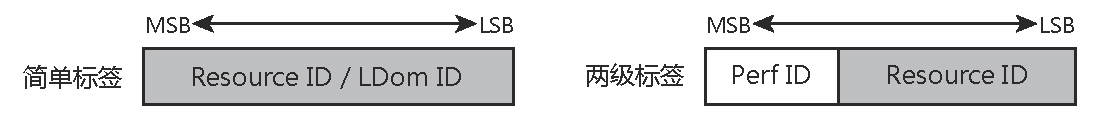
\includegraphics[width=\textwidth]{label/tagging-format}
  \caption[标签格式]{标签格式:分为简单标签与两级标签,
    简单标签直接将逻辑域(LDom ID)映射为标签,
    两级标签将标签分为资源域(Resource ID)和性能域(Perf ID)2部分。
    只有两级标签的性能域部分可以由用户进行修改,
    简单标签或两级标签的资源域(图中阴影部分)只能通过PRM进行修改,
    以保证硬件资源分配不会出现冲突。}
  \label{fig:tagging-format}
\end{figure}

\subsection{如何为请求打标签}
\label{chap:labeladdrspace:tagging}
在确定了标签的格式与内容后,需要将该标签标记到对应的请求上。
在计算机中存在2类请求源:处理器核与I/O设备的DMA引擎,
需要对他们进行分别处理。

\begin{figure}[tb]
\begin{minipage}[b]{0.48\textwidth}
  \centering
  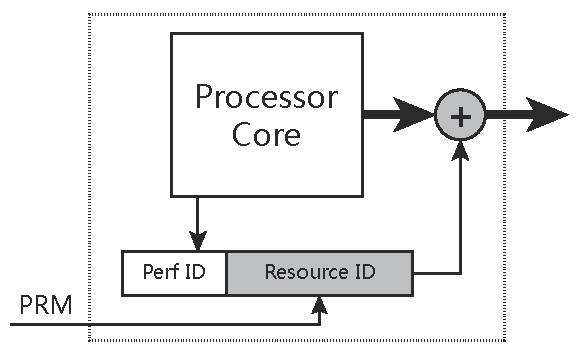
\includegraphics[width=0.9\textwidth]{label/tagging-core-request}
  \caption{为处理器核请求打标签}
  \label{fig:tagging-core-request}
\end{minipage}\hfill
\begin{minipage}[b]{0.48\textwidth}
  \centering
  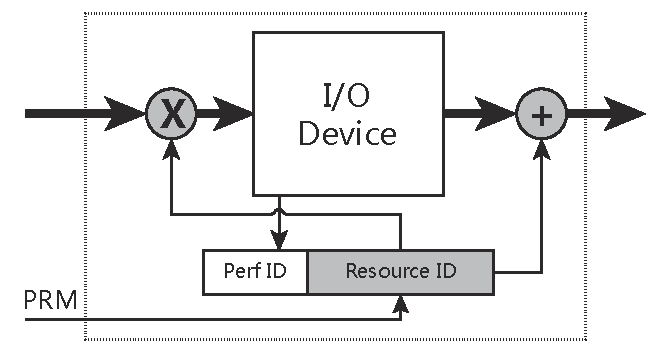
\includegraphics[width=0.9\textwidth]{label/tagging-io-request}
  \caption{为I/O请求打标签}
  \label{fig:tagging-io-request}
\end{minipage}
\end{figure}

\textbf{处理器核}\quad
为标记从处理器核发出的请求,
需要在处理器核内增加1个标签寄存器,将当前正在使用该处理器核的应用标签保存在该寄存器中。
对于简单标签模式,该寄存器对处理器核不可见,只能通过PRM在逻辑域切换时进行修改;
对于两级标签模式,该寄存器的性能域部分对处理器可见,
可以由逻辑域内的操作系统在应用切换时进行修改,而资源域与简单模式下相同,只能由PRM进行修改。
图\ref{fig:tagging-core-request}给出了两级标签模式下,处理器核的请求标记过程:
处理器核发出的请求与标签寄存器的值进行组成,形成带有标签的请求发送到外部;
标签寄存器的资源域部分只能由PRM进行修改,性能域部分可以通过处理器核进行修改。

\textbf{I/O与中断请求}\quad
对于I/O访问,有2种访问模式,即Programmed-I/O(PIO)和Directed Memory Access(DMA)。
对于PIO访问请求,由于I/O请求已经在处理器核端进行了标记,
因此在设备端直接将请求所附带的标签返回即可,但对于DMA请求进行标签标记则需要进行额外的处理。

在介绍PARD的DMA请求标签机制前,先对DMA的工作原理进行简要回顾。
通常DMA请求过程可以分为3个阶段:
首先设备驱动发送``DMA描述符''首地址到DMA控制器,
该``DMA描述符''包含了DMA的缓存信息,例如起始地址、缓存大小、状态;
当初始化完成之后,DMA控制器加载描述符,从中获取每个DMA操作必要的信息并开始数据传输;
最后当所有数据都传输完成后,DMA控制器产生中断告诉CPU数据处理完成。

为了实现DMA请求的标签机制,PARD为每个DMA控制器都增加``标签寄存器'',
如图\ref{fig:tagging-io-request}所示。
在逻辑域创建过程中,PRM对设备进行分配,将逻辑域的资源标签写入到该标签寄存器中。

对于DMA请求的3个步骤,标签寄存器相应的操作如下:

\begin{enumerate}[leftmargin=2\parindent, nolistsep, label=\arabic*)]
  \item 初始化标签寄存器性能域并读取DMA描述符。当设备驱动向DMA引擎写如DMA描述符信息的同时,
        将请求相关的标签性能域部分写入到标签寄存器中,
        DMA引擎将标签寄存器中的值附加到DMA描述符读取请求中;
  \item 标记数据传输请求。当设备的DMA引擎与内存控制器进行收发数据时,
        从其标签寄存器中取出标签,将每个数据传输请求上都打该标签;
  \item 标记中断信号。对于中断,PARD对当前的中断控制器
        (Advanced Programmable Interrupt Controller, APIC)进行适当的扩充。
        在APIC中增加多个中断映射表,其中的每1项都与1个应用标签进行关联。
        这样当DMA引擎产生中断时,应用标签同时被标记到中断请求并发往APIC,
        APIC使用中断请求中的标签来获取相关的映射表,
        根据表中的映射信息将中断请求转发给指定的处理器核。
\end{enumerate}


\section{标签传播}
\label{chap:labeladdrspace:propagation}

标签需要伴随请求在整个生命周期中传播,
这些不同类型的请求需要在各种协议类型的总线上传播(如QPI/HT、AXI、PCI-E等),
其间需要进行多次协议转换,同时会多次穿过各种Cache与Buffer,
本节首先讨论如何扩展现有的总线架构,使其能够传递标签信息,并讨论如何在保证在传播过程中请求与标签始终匹配。
%计算机中的请求主要分为三类:处理器发出的读写请求、I/O设备发出的DMA请求、中断请求。

% TODO: Rewrite this
%\subsection{总线与协议转换}
%
%不同总线上如何实现地址空间

% 总线都是基于包的

% Up-size/Down-size时要注意标签归属


\subsection{多阶段写回请求}
\label{chap:labeladdrspace:propagation:cache}

为了提高性能,计算机数据通路中采用写回(writeback)机制的写操作通常会被拆分成多个阶段。
以共享末级缓存为例,写请求的第1阶段只是将数据写入到缓存中,并将其所属的数据块标记为脏块,
只有当缓存缺失发生且该数据块被选择为替换备选时,数据才会被真正写回到内存。
如果仅使用末级缓存所接收到请求的应用标签作为写回请求的标签,可能会产生标签错误:
引起写回操作数据所属的应用与被写回的数据所属的应用不一致。
为了防止这种情况的发生,需要在共享末级缓存中,
为所有缓存的数据块额外记录其所属应用的标签Owner-DSid,
在第1阶段数据被写入缓存时,将写请求中包含的DSid记录为其Owner-DSid;
当写回操作发生时,使用其Owner-DSid作为传递到下一级的标签。
其他与共享末级缓存行为类似的具有写回机制的部件,都需要应用以上的修改,
才能保证请求在通过该部件后保证应用标签的正确性。


\subsection{一致性协议}

% 侦听和目录两种协议,目前大都使用目录(扩展性原因)
% Source-Snooping 1-2 sockets    <= need reference
% Home-Snooping   4+ sockets
% Directory       64+
PARD使用共享内存多处理器架构,每个处理器都包含自己的私有缓存,
需要使用一致性协议来保证这些私有缓存的一致性。
最常用的保持一致性的方法是基于侦听或基于目录,它们各有优缺点,
基于侦听的方法的优势是响应速度快,所有的请求通过一次广播的请求和回应即可完成,
但它带来的问题是链路带宽占用过大,尤其是当核数增加时,其带宽占用也越来越大。
基于目录的方法主要解决带宽占用问题,通过使用一个公共的目录来记录所有数据的缓存情况,
在需要执行无效操作时,只将请求发送到包含该数据的节点,可以使用点对点的连接,
而无需广播,降低的带宽占用,但与此同时也增加了响应延迟
(需要request/forward/respond三跳)。
通常在四核以下使用基于侦听的方法实现一致性协议,
而更多的核数后需要使用基于目录的方法以降低开销。

% PARD需要对目录项进行修改,以保证正确性
当前处理器核数不断增加,目前普遍的服务器都具有24个处理器核,
这些服务器大都采用基于目录的一致性。
%图\ref{}是基于目录的一致性协议的执行流程,首先....。
由于PARD使用标签的方式区分不同逻辑域的地址空间,系统中存在多个重叠的地址空间,
应用标签是区分这些重叠地址空间的唯一标识。
因此,PARD修改一目录项的定义,将标签信息也加入到目录项中,
在进行地址对比时需要同时对比地址与标签,只有2者同时匹配时才将请求转发到该结点。

% 云计算场景下,每个虚拟机核数较少,可以使用局部侦听的方法实现快速的一致性,
% 同时开销也可控
再次考察基于侦听的一致协议,在节点数较少时性能要高于目录一致性协议,
而随着服务器中核数增加,链路带宽不足以满足侦听需求,
因此才被抛弃,转而使用实现更为复杂的目录一致性协议。
当前多租户云计算场景下,虽然服务器本身具有大量的处理器核(>24),
但每个用户的虚拟机通常只使用很少数量的处理器核。%\cite{}。    % <= TODO: need reference
由于虚拟机之间无内存共享,因此可以只在所有处理器的一个子集中实现一致性,
在这样的范围下,使用基于侦听的一致性可以提高性能,同时由于节点数目较少,
广播开销也不大;特别的,当只使用1个处理器核时,可以忽略所有一致性相关的请求,
进一步降低一致性开销。

PARD的性能标签为以上的一致性协议提供了支持,
即只需要将一致性请求发送到与其标签相同的处理器核,
而无需在全局范围内广播或进行目录查询操作,
通过缩小一致性范围,降低一致性开销并提高性能。

% 即使虚拟机的核数较多,也可以使用局部目录一致性,降低目录存储开销

% 结论,性能标签以及逻辑域抽象,可以实现局部一致性协议,
% 通用逻辑域核数决定一致性协议的类型(甚至是不需要一致性,单核)

\subsection{多内存控制器}

随着处理器核数不断增长,单个内存控制器性能无法满足处理器核的需求,
现有体系结构实现通常包括多个内存控制器,
处理器需要提供一种机制实现物理地址空间在多个内存控制器的分布,
并为请求提供地址解码支持。
以Intel的Xeon架构为例,其使用Source Address Decoder(SAD)
和Target Address Decoder(TAD)实现地址空间管理\cite{intel-xeon-7500}。
其中SAD位于Cache Box(Cbox),负责将请求地址解析到对应的I/O或内存控制器
(对于interleave的地址,则是1组控制器),本节主要讨论对内存地址的解码;
而TAD位于Home Agent(Bbox),负责将请求地址解析为本地地址(主要是处理interleave情况),
并将解析后的地址发送给内存控制器(Mbox)完成访存请求。

SAD的结构如图\ref{fig:intel-7500-sad}所示,
其中包含1个20项的译码表,输入为请求地址,
输出为路由目的地列表,并交给Router模块转发请求。
在Intel的这种体系结构下,请求路由是由请求地址决定。
在PARD体系结构下,需要综合考虑请求地址与应用标签,
因此需要对译码表进行扩充,在系统中预留多组译码表(组数由支持的最大逻辑域数量决定),
这些译码表使用逻辑域标签进行索引,当PRM决定在某个处理器核上运行逻辑域时,
将该逻辑域对应的译码表加载到处理器中,
这样保证该处理器核在做地址译码时使用对应用逻辑域的地址分配。

\begin{figure}[tb]
  \centering
  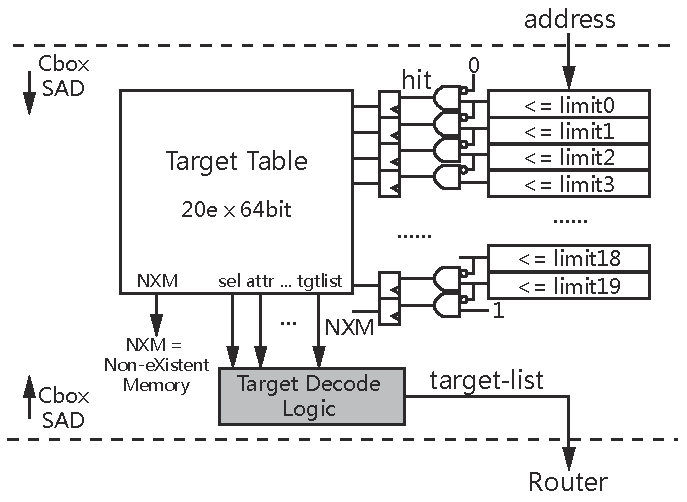
\includegraphics[width=0.7\textwidth]{label/intel-7500-sad}
  \caption[Intel SAD地址译码]{Intel SAD地址译码\cite{intel-xeon-7500}}
  \label{fig:intel-7500-sad}
\end{figure}


\section{PARD模拟器}
\label{chap:labeladdrspace:nohype}

利用本章所设计的性能标签与相应的标签传播机制,
在整个计算机体系结构内能够识别出来自不同应用的请求。
本节基于模拟器,介绍标签机制的具体实现,
并讨论如何该架构下实现全硬件支持的虚拟化技术,提供PARD体系结构的逻辑域抽象。

PARD模拟器是基于gem5\cite{binkert_gem5_2011}开发的时钟精确(cycle-accurate)
体系结构模拟器\footnote{PARD-gem5模拟器已在LGPL协议下开源,地址https://github.com/fsg-ict/PARD-gem5},
它使用x86指令集与Classic Memory内存模型,
能够支持atomic、timing-simple和detail 3种模型进行仿真。
它模拟了1台四核x86服务器,具体配置参数如表\ref{tab:pard-sim-setup}所示,
主要包括:
处理器核使用乱序四发射,工作频率为2GHz,
具有分离的指令与数据缓存,容量均为64KB;
4个处理器核共享4MB的末级缓存(16路组相连)和1个DDR3内存控制器,内存容量为8GB;
在I/O方面,服务器提供4个IDE控制器,每个控制器上挂载2个磁盘。

\begin{table}[b]
  \centering
  \begin{minipage}[t]{0.9\linewidth}
  \caption{PARD模拟器参数}
  \label{tab:pard-sim-setup}
    \begin{tabular*}{\linewidth}{rl}
      \toprule[1.5pt]
      CPU                  & 4 4-issue Out-of-Order X86 cores, 2GHz\\
      L1-I/core            & 64KB 2-way, hit = 2 cycles \\
      L1-D/core            & 64KB 2-way, hit = 2 cycles \\
      Shared LLC           & 4MB 16-way, hit = 20 cycles \\
      \hline
      DRAM                 & 8GB DDR3-1600 11-11-11, 4Gbit chip (Micron MT41J512M8) \\
                           & 1 channel, 2 ranks/channel, 8 banks/Rank \\
                           & Burst Length = 8, Row buffer = 1KB \\
                           & tCK=1.25ns, tRCD = 13.75ns, tCL = 13.75ns, tRP = 13.75ns, tRAS = 35ns, \\
                           & tRRD = 6ns \\
      \hline
      Disks                & 4-channel IDE controller, 8 disks \\
      \hline
      Platform             & 100MHz X86 core, 16MB DRAM, 32MB Flash Storage \\
      Resource             & 1 Ethernet adaptor  \\
      Manager              & 4 control plane adaptors (CPA) \\
      (PRM)                & Firmware: tailored Linux kernel 2.6.28.4 with Busybox \cite{busybox} \\
      \hline
      Server OS            & Gentoo Linux with kernel 2.6.28.4 \\
      \hline
      Workloads            & memcached \cite{memcached}, SPEC-CPU 2006 \cite{cpu2006} \\
                           & MicroBenchmark: CacheFlush \& DiskCopy \\
      \bottomrule[1.5pt]
    \end{tabular*}\\[2pt]
  \end{minipage}
\end{table}

模拟器在处理器核上增加了标签寄存器,并扩展了模拟器中的请求(packet)类型,
实现应用标签的传播,
第\ref{chap:labeladdrspace:simimpl}节将详细介绍为实现PARD的性能标签所进行的修改。
模拟器还在处理器末级缓存、内存控制器与IDE控制器上增加了可编程控制平面,
并对硬件资源数据平面所提供的功能进行管理,
第\ref{chap:hwresman}章将详细介绍控制平面相关内容。
模拟器中同时模拟了基于x86体系结构的PRM,其主要配置包括:
100MHz的x86处理器核、16MB内存、32MB存储、串口和以太网控制器,
以及用于控制平面适配器。
控制平面网络基于gem5模拟器中总线逻辑实现,连接以上3个控制平面到PRM的控制平面适配器。
PRM上运行经过裁剪的Linux系统,基于内核版本2.6.28.4和Busybox\cite{busybox}实现。

该模拟器能够模拟PARD体系结构的关键特性,实现将PARD服务器划分为最多4个逻辑域,
并运行未经修改的Gentoo Linux(内核版本2.6.28.4);
典型的Benchmark应用,如SPEC CPU\cite{cpu2006};
以及CloudSuite\cite{Ferdman:2012:cloudsuite}的部分组件,如memcached\cite{memcached}。


\subsection{性能标签实现}
\label{chap:labeladdrspace:simimpl}

% 实现打标签做的事情
如之前章节所介绍,标签机制包含2个部分,即标签的标记与传播。
为实现标签标记,PARD模拟器修改了x86控制器寄存器的定义,
在其中增加了1个16位的标签寄存器,其中低12位为资源域,高4位为性能域;
在x86指令集中增加了2条MOV指令,实现标签寄存器性能域与通用寄存器之间的数据传递。

gem5模拟器不同组件之间使用请求包(packet)类型传递请求与数据,
为实现标签传播,PARD模拟器扩展了请求包类型的定义,
在其中增加了16位的标签域DSid用于请求标记。
不同组件之间请求包是通过端口(port)进行传递,
gem5模拟的x86处理器核通过4个端口与内存子系统相连,分别是
I-Cache Port、D-Cache Port、ITB Walker和DTB Walker,
通过修改这些端口所在部件的逻辑,在发送请求前,
将标签寄存器的值记录到请求包类型的DSid域中,实现请求标记。
另外,Classic Memory内存模型下,使用基于侦听的一致性协议,
为保证一致性的正确性,PARD模拟器还修改了处理器核侦听端口的逻辑,
另其只接收并回复来自相同应用标签的侦听请求。

% 实现标签传播做的事情
由于gem5模拟器在整个系统中都使用请求包和端口的方式实现组件连接,
因此只需要在请求包创建时标记其标签,而无需进行协议转换、位宽转换等工作。
在真实系统中,请求需要在不同协议之间进行转换,
在实现标签传播时需要额外考虑这些因素。
标签在处理器末级缓存中传播是模拟器实现时需要重点考虑的问题,
PARD模拟器使用第\ref{chap:labeladdrspace:propagation:cache}节介绍的方法,
对gem5的Cache模块进行修改,
通过在Cache的TagArray中增加Owner-DSid,实现标签的正确传播。


% 考查Hypervisor的功能,实现资源划分,与操作系统加载
通过以上修改,已经在PARD模拟器上实现了性能标签机制,
下面将讨论如何在该机制下实现无Hypervisor的全硬件支持虚拟化功能。
考查Hypervisor的功能,它主要负责2方面的任务:
一是实现系统内资源的划分,例如vCPU调度实现处理器资源划分,
通过EPT机制实现内存地址空间划分,通过虚拟设备的方式实现I/O资源划分;
二是操作系统加载与BIOS模拟,在虚拟机中模拟出操作系统执行所需的软件环境。

% 现在有标签后,怎么利用标签做memory/io划分
PARD的性能标签在硬件上为资源划分提供了良好的支持。
通过处理器标签寄存器,实现处理器资源的划分,为简化实现,
当前只为每个逻辑域固定分配一个处理器核。
内存控制器可以直接使用访存请求上所附带的标签,
通过增加按应用区分的地址映射实现内存资源的划分。
对于I/O资源,由于当前模拟器配置下只有4个处理器核,最多只能支持4个逻辑域,
因此使用固定划分的方式,为每个逻辑域分配1个IDE控制器及与之连接的2块磁盘。
具体包括2个方面的修改:
其一是在I/O总线上实现与内存控制器相类似地址映射,实现I/O资源的划分;
其二是在IDE控制器上增加标签寄存器,记录使用该控制器的逻辑域,用于标记DMA请求。
通过以上修改,实现硬件支持的资源划分。

% 操作系统加载又怎么做
对于操作系统加载,gem5模拟了操作系统加载的过程:
使用ELF Loader直接将Linux操作系统内核镜像加载到内存指定的位置,
然后根据用户配置文件生成BIOS配置表写入到内存中;
在此之后,对处理器状态进行初始化,并将PC寄存器指向内核的入口;
模拟开始后,处理器直接执行操作系统内核代码。
PARD模拟器在此基础上进行扩展,分别在4个逻辑域内执行以上流程,
完成逻辑域内的操作系统加载。
该过程需要模拟器本身参与,在实际的系统中该工作要由运行在PRM中的固件代码完成,
受到gem5设计与性能上的限制,部分PRM固件的功能被移动到了模拟器中实现,
这是在模拟器功能模拟上的折中,第\ref{chap:impl}章的FPGA原型系统对该问题进行了修正,
使用了真实的PRM来实现以上功能。

% 实验结果
经过以上修改,
PARD模拟器能够在无需软件Hypervisor支持下同时在多个逻辑域内运行操作系统,
图\ref{fig:pard-nohype-simulator}给出了4个逻辑域启动操作系统并运行应用时内存带宽与Cache容量的变化。
该模拟器实验证明,能够在模拟的x86体系结构下实现性能标签机制扩展,
并利用该机制实现无需软件Hypervisor支持的全硬件虚拟化功能。

\begin{figure}[tb]
  \centering
  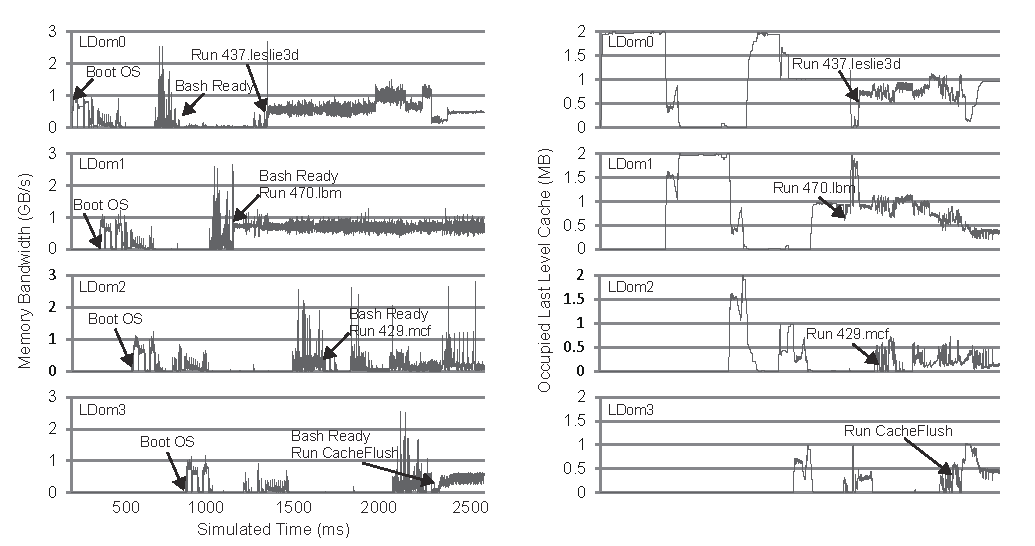
\includegraphics[width=\textwidth]{label/pard-nohype-simulator}
  \caption{动态划分PARD服务器为4个逻辑域,并在其中运行操作系统与应用}
  \label{fig:pard-nohype-simulator}
\end{figure}


\section{业界最新进展}
\label{chap:labeladdrspace:intel-rdt}

对于本章所分析的共享环境下多应用硬件资源竞争产生干扰的问题,
Intel从Xeon E5-v3系列处理器开始提供Resource Director Technology(RDT)\cite{intel-rdt}
方案来解决该问题。
如图\ref{fig:intel-rdt-overview}所示,该方案的硬件基础是资源监控与资源分配控制机制,
同时提供基于``监控$\rightarrow$策略$\rightarrow$控制''
组合的闭环方式来实现应用感知的资源管理框架。
其中资源监控提高了资源使用情况的能见度,使得资源利用率可以被跟踪,
同时可以侦测到应用性能随资源的变化,为上层的资源调度提供数据基础;
而硬件支持的资源分配控制机制,使得上层软件可以控制对硬件共享资源的使用。

% Intel RDT Overview
\begin{figure}[H]
  \centering
  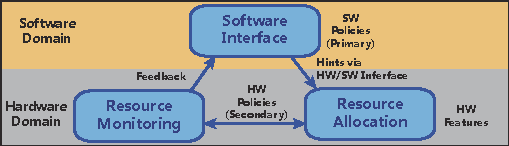
\includegraphics{x86eval/intel-rdt-overview}
  \caption[Intel Resource Director Technology (RDT) 技术示意图]{
    Intel Resource Director Technology (RDT)技术:硬件提供资源监控与分配功能,
    软件负责对资源使用进行调度,实现资源按需求动态分配。}
  \label{fig:intel-rdt-overview}
\end{figure}

目前Intel已经将RDT方案应用到共享末级缓存和内存控制器中,
在E5-v2系列中提供CMT(Cache Monitoring Technology)
和MBM(Memory Bandwidth Monitoring)功能(2013年),
实现按应用区分的缓存容量监控、以及全局内存带宽的监控;
在E5-v3系列中增加了CAT(Cache Allocation Technology)功能(2015年),
实现按应用区分的缓存容量划分;
在E5-v4系列中扩展MBM功能(2016年),
实现按应用区分的内存带宽监控。

CMT和MBM技术实现应用区分的缓存容量与内存带宽监控的流程如图\ref{fig:intel-cmt-flow}所示。
操作系统或VMM首先为执行实体(如线程、进程或虚拟机)分配资源编号RMID,后续的监控结果都将
以RMID的形式进行汇报。在OS/VMM执行调度并进行上下文切换时,将被调度实体的的RMID写入到目标
处理器核对应的寄存器中。OS/VMM可以随时通过RMID查询各个执行实体的资源使用情况,如共享缓存
占用或访存带宽等信息。

% Intel CMT Flow
\begin{figure}[H]
  \centering
  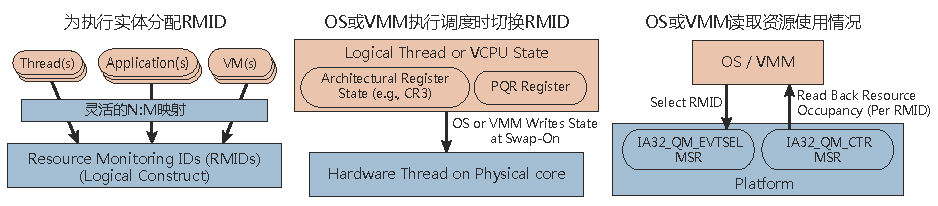
\includegraphics{x86eval/intel-cmt-flow}
  \caption[Intel Cache Monitor Technology (CMT) 技术流程]{Intel CMT技术流程:
   (1)为线程、应用或虚拟机等执行实体分配资源编号RMID;(2)将包含RMID的PQR寄存器
   保存在线程TCB或虚拟机VCPU中,并在执行上下文切换时写入到处理器核对应的物理寄存器中;
   (3)根据RMID使用MSRs寄存器获取共享资源使用情况。}
  \label{fig:intel-cmt-flow}
\end{figure}

CAT技术为OS/VMM提供了控制末级共享缓存容量的功能,如图\ref{fig:intel-cat-flow}所示,
当该功能被开启后,应用将只能使用分配给它的Cache容量,实现路划分。
路划分策略是以COS为粒度进行指定,OS/VMM首先为某一COS制定路划分策略,并将该COS关联到使用
该策略的执行实体中,并在上下文划分时将被调度实体的COS写入到处理器核对应的寄存器中,
共享缓存根据COS对应的策略来进行缓存替换操作。

\begin{figure}[H]
  \centering
  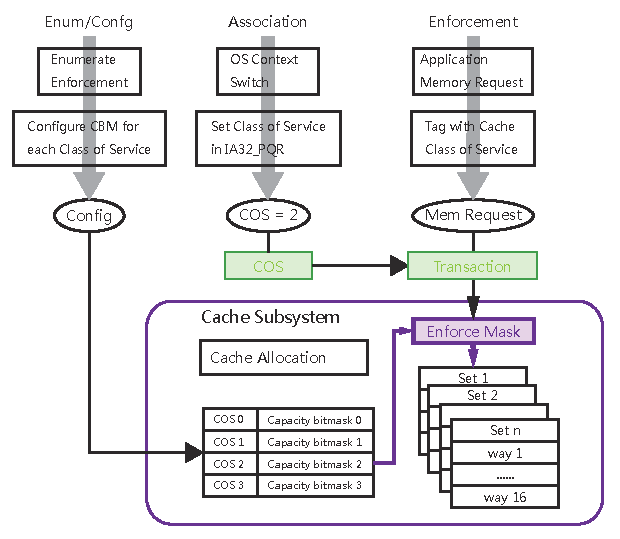
\includegraphics[height=8cm]{x86eval/intel-cat-flow}
  \caption[Intel Cache Allocation Technology (CAT) 技术流程]{Intel CAT技术流程}
  \label{fig:intel-cat-flow}
\end{figure}


\section{小结}

本章根据区分化服务的需求,分析了现有计算机体系结构的不足,提出使用标签传递软硬件信息,
让硬件支持区分化服务。并给出了性能标签方案,包括标签的生成与传播,
同时使用模拟器验证了标签机制的可行性,并利用标签机制实现了全硬件支持的虚拟化。
最后,介绍业界在应用区分化服务方向上的最新进展,
Intel在其Xeon E5-v3(2015年)/v4(2016年)系列处理器提出的RDT技术,
使用与本章所述性能标签相似的方案,
实现处理器末级缓存与内存控制器的性能监控、以及缓存容量划分。
未来数据中心计算机体系结构,标签将与地址具有相同的地位,
会成为体系结构内基本的元素。



%%% Local Variables:
%%% mode: latex
%%% TeX-master: t
%%% End:

\chapter{硬件资源共享管理方法}
\label{chap:hwresman}

由于缺少有效的硬件资源共享管理机制,现有服务器体系结构不能很好的在共享场景中工作:
不同应用无管理的访问共享硬件资源,产生资源竞争并造成严重的性能干扰,进而影响应用性能。
大量研究尝试解决不同硬件层次上干扰所带来的性能问题,
如Cache容量划分\cite{kasture_ubik:_2014, sanchez_vantage:_2011, sanchez_zcache:_2010, qureshi_utility-based_2006}
或访存调度\cite{muralidhara_reducing_2011}等。
但受到数据中心海量应用\cite{Reiss_googletrace_2012}且应用组合不断变化的特征影响,
这些方法在数据中心内并没有发挥应有的作用,主要有3个方面的原因。
首先,这些方法通常只针对单一硬件资源的竞争,而数据中心应用会在不同的硬件层次上产生竞争;
第二,由于没有统一的框架与接口,无法通过多种方法组合的方式解决不同硬件层次上的竞争;
最后,为每种可能的硬件资源竞争场景都单独设计资源管理方法,
在数据中心这种海量应用的共享场景下是不切实际的。

基于以上3个问题,本章提出一种通用硬件资源管理方法与架构,
通过统一的接口将不同的硬件上不同的机制、策略结合,
使用软件可编程的方式对硬件资源管理方法进行调整,
包括基于``控制平面''的策略可编程和``数据平面''的机制可编程,
以支持数据中心复杂多变的应用场景。
具体内容安排如下:
首先分析通用硬件资源管理的动机,然后针对2类主要硬件资源Cache和内存控制器分析其资源抽象,
提出基于``控制平面''与``数据平面''的资源抽象方法,
具体设计控制平面与数据平面,并使用模拟器对控制平面的效果进行评估,
数据平面由于性能问题无法使用模拟器进行评估,将在第7章中使用FPGA 原型对其进行评估。


\section{问题分析}

\begin{figure}[tb]
  \centering
  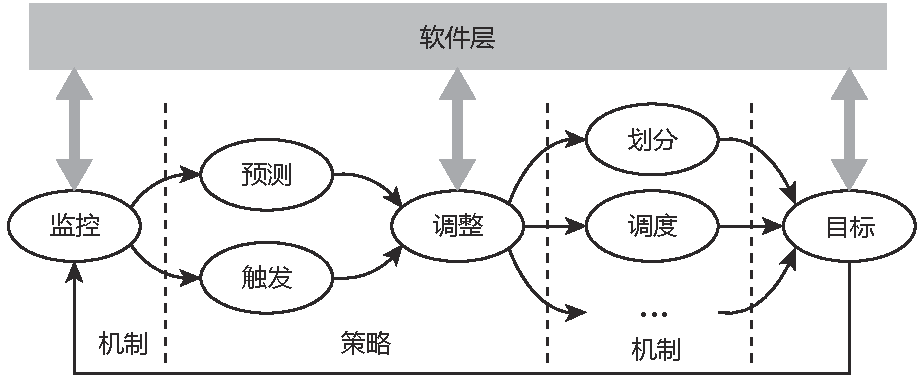
\includegraphics[width=0.8\textwidth]{hwres/resource-manage-flow}
  \caption{资源管理流程模型}
  \label{fig:resource-manage-flow}
\end{figure}

在计算机系统中,通常使用反馈调节的方式实现应用服务质量保障。
根据应用的服务质量需求制定调节目标,可能是单目标或复合的多目标;
采集系统中与目标相关的状态信息,通过预测或条件触发的方式对可能发生的违例进行监控;
当违例发生时,或预测到即将发生违例时,通过调节机制对资源进行重新分配,使系统满足目标。
该过程如图\ref{fig:resource-manage-flow}所示,
除以上所述流程外,通常应用层还会提供目标、监控与调整的接口,用于对整个流程进行控制。

%基于该模型,现有部分软件层次的工作\cite{controlwave2002, Hoffmann:2015, Hoffmann:2014}
%设计了不同的反馈调节机制,实现以QoS或能耗为目标的资源管理,
%本节主要关注如何在硬件体系结构层次利用该模型实现QoS保障的资源管理。

现有服务质量保障工作都是以该模型为基础进行设计。
以Intel RDT技术(参见第\ref{chap:labeladdrspace:intel-rdt}节)为例,
它通过CMT与MBM技术提供处理器末级缓存容量、访存带宽的监控,
在软件层次根据监控结果对资源分配进行调度,
最后通过资源调整接口实现资源重新分配,
目前RDT只提供了CAT技术实现处理器末级缓存容量的划分。
考查其他软硬件服务质量保障技术\cite{tang_reqos:_2013,yang_bubble-flux:_2013,Zhang:2009,herdrich_rate-based_2009,Jigsaw:2013,kasture_ubik:_2014,Nesbit:2006,mutlu_stall-time_2007},
它们虽然针对不同的硬件资源、提供不同机制或策略,
但它们都符合图\ref{fig:resource-manage-flow}所示的资源管理流程模型,
表\ref{tab:resman-compare}列举了这些工作与模型的映射关系。

\begin{table}[htb]
  \centering
  \begin{minipage}[t]{\linewidth}
  \caption{资源管理相关工作}
  \label{tab:resman-compare}
    \begin{tabular*}{\linewidth}{ccp{2.2cm}<{\centering}p{5.6cm}}
      \toprule[1.5pt]
      \textbf{相关工作}                        & \textbf{QoS指标} & \textbf{监控机制}   & \textbf{QoS保障策略}     \\
      \midrule[1pt]
      ReQoS\cite{tang_reqos:_2013}             & IPC              & 性能计数器 & 基于编译和运行时的应用执行管控(throttling)     \\
      Bubble Flux\cite{yang_bubble-flux:_2013} & IPC              & 性能计数器 & 基于Linux信号(SIGSTOP \& SIGCONT)的执行管控    \\
      \hline
      Zhang \emph{et.al.}\cite{Zhang:2009}     & 执行时间         & \emph{N/A} & 硬件执行管控,\emph{e.g.} duty-cycle modulation  \\
      Rate-Based QoS\cite{herdrich_rate-based_2009} & IPC、执行时间    & 性能计数器 & 硬件执行管控,\emph{e.g.} clock modulation, DVFS \\
      Intel RDT\cite{intel-rdt}                & 缺失率、带宽     & CMT、MBM                               & Cache容量划分,CAT                                 \\
      Jigsaw\cite{Jigsaw:2013}, Ubik\cite{kasture_ubik:_2014} & 缺失率、长尾延迟 & UMON\cite{qureshi_utility-based_2006}  & Cache容量划分,Vantage\cite{sanchez_vantage:_2011} \\
      FQ-VT\cite{Nesbit:2006}                  & IPC、访存延迟        & \emph{N/A}  & Fair-Queuing访存调度    \\
      STFM\cite{mutlu_stall-time_2007}         & 访存带宽、延迟       & \emph{N/A}  & Stall-Time Fair访存调度 \\
      \bottomrule[1.5pt]
    \end{tabular*}\\[2pt]
  \end{minipage}
\end{table}

虽然以上这些方法具有相同的资源管理模型,在监控与调整方面有通用的地方,
但由于接口问题无法共存。
同时它们都只面向于特定的场景,
在数据中心这种应用众多且需求各异的通用场景下,任何单一的方法都无法适用。
在这种情况下,为服务器提供多种机制和策略,对它们进行统一的管理,
根据应用负载的不同,选择适当的机制或策略的组合是更为合适的方案。
但由于缺少统一的接口现有方案无法进行统一管理,更不能实现协同工作。

该问题与网络领域中网络设备管理存在相似性。
例如交换机、路由器等网络设备,虽然其具有相同的``存储$\rightarrow$转发''功能模型,
但不同厂商生产的网络设备相互之间并不兼容,由于接口、协议等问题不能协同工作。
而SDN/OpenFlow的出现,为这些网络设备提供了统一的管理协议(OpenFlow),
不同的网络设备可以协同工作,并通过SDN在统一的控制平面架构下对整个网络进行管理;
同时利用SDN可编程特性,灵活部署新的策略,根据应用需求变化调整网络架构,
使得网络资源的管理更为灵活。

在体系结构内,不同的硬件部件相当于不同网络设备,同样需要一个统一架构实现资源管理,
该架构需要具有以下特性:

\begin{enumerate}[leftmargin=2\parindent, nolistsep, label=\arabic*)]
  \item 能够适应不同类型的硬件资源
  \item 能够很容易的集成现有资源管理机制与策略
  \item 灵活的可编程策略实现
  \item 灵活的可编程机制实现
\end{enumerate}

本章所提出的通用硬件资源管理方法使用``控制平面''和``数据平面''抽象描述所有硬件资源(特性1,第\ref{chap:hwresman:res}节),
通过基于控制表的可编程控制平面实现策略可编程(特性3,第\ref{chap:hwresman:cp}节),
通过基于处理器的可编程数据平面实现机制可编程(特性4,第\ref{chap:hwresman:dp}节),
现有的资源管理机制可通过数据平面集成到系统中,而资源管理策略可通过控制平面实现集成(特性2)。



\section{硬件资源抽象}
\label{chap:hwresman:res}

% 硬件资源的``控制平面''与``数据平面''抽象
计算机内的硬件资源主要可以分为基于容量的资源和基于流量的资源2类,
例如,共享缓存、处理器核、以及硬盘空间是基于容量的资源,
总线带宽、访存带宽、或网络带宽是基于流量的资源。
这2类资源在管理上使用不同的参数与策略,PARD使用数据平面与控制平面抽象对其进行统一,
实现这些不同类别硬件资源的统一管理。
其中数据平面用于执行请求操作,如处理器末级缓存对DataArray/TagArray的管理、替换策略实现等;
对于内存控制器,其数据平面负责接收上层访存请求、将物理地址转换为DRAM地址以及访存请求调度等。
而控制平面用于对数据平面的策略进行管理,
例如对处理器末级缓存数据平面中替换策略的管理、命中信息统计;
内存控制器数据平面的地址映射与调度策略则是由控制平面进行管理。

% 控制平面与数据平面分离:控制平面是策略接口的抽象,数据平面的机制的实现
数据平面基于硬件原有功能实现,并在此基础上提供机制的可配置功能,
将更多的硬件细节通过控制平面暴露给软件进行管理;
控制平面对数据平面所提供的机制进行管理,如提供监控信息的访问、资源调整的接口,
同时为上层提供策略编程接口,如资源访问冲突发现与预测功能。
通过这种抽象方法,将硬件的资源管理机制与具体的策略分离,
针对数据中心应用数量众多且组合多变的需求,
可以在硬件上实现多种资源管理机制(如监控、划分、调度等),
并通过软件编程的方式实现不同的策略以应对不同的应用需求。

% 静态数据平面设计不能很好的适应数据中心多变的场景
以上方案中,控制平面可编程主要体现在其对数据平面所提供功能的控制,
而数据平面所提供的功能在其设计完成后即已确定,如果需要增加额外的功能,
则需要对数据平面进行重新的设计,并对控制平面暴露相应的接口。
因此,控制平面的可编程能力受到数据平面所能提供功能的限制。
然而在实际数据中心场景中,应用会对底层的硬件不断提出不同的需求,
如更换处理器末级缓存替换策略、更改内存控制器的地址映射方式与调度策略、
为I/O控制器增加数据加密或压缩的功能等。
静态的数据平面设计不能很好的满足这类需求,需要修改其硬件逻辑才能实现,
而这需要很长的周期,无法适应数据中心这种需要不断变化的场景。

% 通过在数据平面也增加可编程机制,更灵活的资源管理
在学术界中,已有一些研究通过在硬件上增加可编程机制,
实现根据应用需求对硬件策略进行调整的功能。
如体系结构领域已经提出在内存控制器\cite{bojnordi_pardis:_2012, martin2009, kornaros2003}、
Cache与一致性协议\cite{kuskin1994, reinhardt1994, impulse1999, pong1998}
上使用可编程逻辑来提供更灵活的功能,
但这些只考虑了如何为单一应用提供更多的可编程支持,
不能很好的在数据中心这种多应用场景下使用。
在网络领域中也有工作提出在SDN数据平面上增加可编程逻辑的方案,
以提高SDN数据平面的可编程性\cite{p4_2014, song2013, jeyakumar2013, sivaraman2013},
通过数据平面的重编程,达到对更多数据包的检测与处理的目的。
考查现有硬件部件的实现,它们通常使用多阶段流水的方式对输入请求进行处理,
可以借鉴现有这些研究的方法,使用可编程机制替代硬件资源中部分流水级,
使用执行固件代码的方式对硬件部件的请求进行处理,
并通过更新数据平面处理器固件的方式实现数据平面功能的扩展,
以增强计算机体系结构的可编程灵活度,
使其能够适应更加复杂多变的数据中心应用场景。

\begin{figure}[tb]
  \centering
  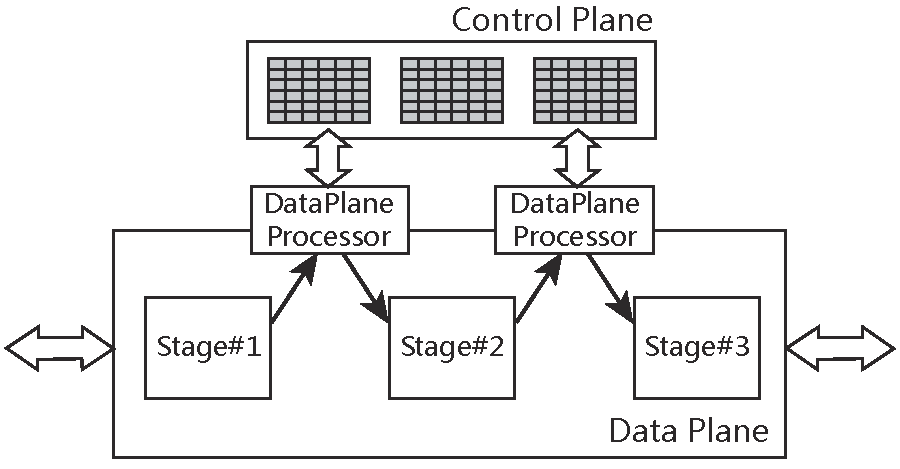
\includegraphics[width=0.6\textwidth]{hwres/pard-res-abstract}
  \caption{可编程硬件资源管理架构}
  \label{fig:pard-res-abstract}
\end{figure}

% 实现的架构是什么样子的
基于以上硬件资源抽象模型,以及数据平面和控制平面的可编程设计,
本章提出的可编程硬件资源管理架构如图\ref{fig:pard-res-abstract}所示。
按照上文所述硬件资源抽象模型,硬件资源被划分为数据平面与控制平面2部分:
在数据平面的请求处理器流水线中,硬件逻辑将自身的配置参数暴露给控制平面进行控制,
同时通过增加可编程处理器,使用固件代码进行请求处理,实现数据平面的机制可编程;
在控制平面,将数据平面中所有可编程、可配置的机制以控制表的形式进行维护,
并提供给用户,实现硬件资源的策略可编程。

% 难点是什么
%  - 数据平面:选用什么样的可编程逻辑,关键路径,降低开销
%  - 控制平面:什么样的抽象,什么样的接口
要实现以上可编程资源管理架构,其核心即为数据平面与控制平面的设计。
而数据平面设计的关键在于其内部可编程处理器的设计,使其能够
\textbf{(1)灵活的嵌入到不同硬件资源的数据平面中};
同时可编程处理器位于硬件资源数据平面的数据通路上,需要保证
\textbf{(2)额外增加的逻辑不会对系统性能造成影响}。
与之对比,控制平面并不在数据通路的关键路径,因此性能方面无需过多考虑,
而更多是采用何种方式实现数据平面抽象,以及
\textbf{(3)如何为上层应用提供灵活的策略接口}。
如何\textbf{(4)实现数据平面处理器运行时可编程}
是实现该架构需要解决的另一个重要问题。

在介绍数据平面与控制平面的具体设计之前,首先以内存控制器和缓存控制器为例,
讨论如何将本章所提出的可编程资源管理架构应用到现有硬件。

%本章后续章节将依次介绍PARD体系结构中控制平面与数据平面的设计,
%并通过模拟器对控制平面的效果进行验证,由于
%使用模拟器对控制平面以及缓存划分功能进行验证,数据平面由于模拟速度太慢,直接在FPGA平台上进行验证,更多关于FPGA平台的信息参见第\ref{chap:impl}章。

\subsection{内存控制器}
当前的处理器芯片通常会集成2个到4个独立的内存控制器,每个控制器使用独立的内存通道。
每个内存通道连接到多个可并行访问的rank,
而每个rank又是由多个共享地址与数据总线的二维存储阵列(bank)组成。
内存控制器的主要工作就是接收上游的读写请求,并将其转换为下游的DRAM命令,完成数据传输。
以内存控制器作为数据平面,可以在地址映射和访存调度2个位置增加可编程功能,
并在控制平面提供对地址映射与访存调度的控制。

\textbf{地址映射}\quad
地址映射分为2部分,
首先是通过处理器的页表机制实现了从虚拟地址空间到物理地址空间的映射,
虚拟化场景的出现在其基础上又增加了扩展页表EPT机制,
额外增加了从虚拟机物理地址到主机物理地址的映射。
内存控制器将处理器的物理地址空间映射到DRAM阵列中,
通常使用静态地址映射,
通过某种固定的规则将物理地址空间映射到DRAM的bank、row和column中。

在PARD中,通过在内存控制器中增加MMU模块,使用映射表将不同应用标签的访存请求进行隔离。
但这种方式实现的是固定的地址映射机制,即只能进行连续的大块地址分配,
无法实现EPT等技术所支持的细粒度内存空间管理。
为解决该问题,通过修改静态的MMU模块,将其替换为可编程处理器,
在其中编写软件代码实现地址空间的映射。
通过这种方式除了可以完成PARD中MMU的功能外,还可以实现更细粒度的空间管理,
也可以实现现有虚拟化平台中常见的基于内容的内存空间压缩机制,
在硬件层面实现更复杂的如数据加密、敏感词过滤等高级功能,

\textbf{访存调度}\quad
在PARD的内存控制平面中,能够实现对访存调度的控制,
而通过在数据平面增加可编程处理器的方式能够实现更为灵活的调度策略。
也可以像PARDIS\cite{bojnordi_pardis:_2012}工作一样,
将处理器加入到内存控制器内部的请求调度模块中,根据不同应用的需求实现不同的DRAM调度策略。

本文所完成的FPGA原型系统并没有包含以上这些高级功能,
而只实现基本的地址映射,用于验证其资源和性能开销,
以上这些功能可以做为未来PARD可编程数据平面方向的扩展研究。

\subsection{缓存控制器}
缓存控制器(Cache)的功能是对到达的请求进行缓存操作,
使用不同的替换策略,对数据访问热度进行预测,以提高访存命中率,提高系统性能。
Cache的核心主要包括TagArray、DataArray和替换策略3个部分。
以Cache作为数据平面,可以在容量划分与替换策略2个角度增加可编程功能,
并在控制平面提供对Cache状态的监控以及划分和替换策略的管理。

\textbf{容量划分}\quad
传统的Cache并没有提供容量划分功能,
因此不同应用在共享Cache上运行会造成不同程度的干扰。
Intel RDT中的技术\cite{intel-cat}在Cache上增加了按路的缓存容量划分机制。
但按路划分并非适合所有的应用,可以通过使用处理器替换固定的Set/Way映射方式,
根据应用实现更为灵活的缓存容量划分方式。

\textbf{替换策略}\quad
与容量划分的需求类似,不同应用的访存模式不同,
固定的缓存替换策略并不能很好的适应所有应用。因此使用处理器与软件替换策略,
与PARD的应用区分机制结合,可以实现更为灵活高效的缓存。

\section{控制平面设计}
\label{chap:hwresman:cp}

%控制平面是在硬件之外增加的一层,对硬件的行为进行控制,
%同时可以在必要时对发送到硬件的请求进行额外的处理,如地址变换、请求无效等。
%由于控制平面能够感知到硬件处理的所有请求,因此可以实现实时性能监控与反馈,
%由于控制平面能够对硬件行为进行控制,因此可以实现资源调整机制。

%资源监控是实现硬件资源可管理共享的第一步,要实现好的共享管理策略,必需对系统当前的资源分配情况、应用性能进行细粒度、实时的监控。
%目前监控主要是软件和硬件2个方面,由于
%
%PARD可以按应用进行控制,
%
%Intel使用Performance Counter机制实现资源监控,通过软件设定监控的事件类型,
%并指定计数器上限,当该事件的计数达到该上限时发起中断通知,

\subsection{控制表抽象}
\label{chap:hwresman:cp:table}

% 数据平面屏蔽硬件之间的差异,控制平面做数据平面的接口
% 数据平面需要控制参数、存储状态
% 因此控制平面中使用参数表与状态表做这件事
% There are various hardware components that behave differently
% and use DS-id tags in different ways as well, e.g., LLC using DS-id
% for capacity allocation while memory controller using DS-id for
% bandwidth allocation.
% We devise a basic control plane structure for a variety of components.
% 表的具体结构,使用前一章提供的DS-id做索引,由数据平面对其列进行解析
硬件部件有不同的行为,但这些行为的不同通过数据平面的抽象已经屏蔽,对于控制平面来说,
它只是需要保存数据平面的实时状态,同时为数据平面的机制提供所需的参数。
基于这2个需求,控制平面使用控制表作为数据平面的接口,其中包括:
参数表(parameter table,ptab),用于记录数据平面机制所需的参数;
状态表(statistics table,stab),用于记录数据平面的状态信息。
通过第\ref{chap:labeladdrspace}章所提供的标签机制,控制平面能够区分出来自不同应用的请求,
以上2个控制表都使用该应用标签(DS-id)进行索引(控制表行),
控制表中具体记录何种控制参数与状态信息由硬件资源及其数据平面决定,
用户通过修改2个控制表实现按应用区分的数据平面控制与状态获取。

硬件模块在收到请求后,使用请求中的应用标签查询参数表,获取需要的参数,
并与请求一同传递到数据平面,由于参数表使用应用标签进行区分,
因此来自不同应用的请求具有不同的参数;
数据平面根据控制平面传递的参数对请求进行区分处理,并在请求处理完成后,
将请求的应用标签与更新的状态信息送回控制平面,由控制平面完成状态表信息的更新。

所有的控制平面通过控制平面网络连接到PRM,由PRM实现对控制表的集中式管理,
包括对不同硬件资源参数调整以及状态查询。
为了保证性能监控的实时性,PRM需要不断轮询所有的控制平面,
而在实际应用场景中,性能违例只是突发事件,使用轮询的方式进行检测是对PRM资源的浪费。
%是只关心其中的部分状态信息,使用轮询的方式过于浪费,
因此在控制平面中还提供一种条件触发机制来降低轮询所带来的开销,具体流程如下:
1)PRM将当前关心的应用\&状态组合、通知条件提供给控制平面;
2)控制平面在更新状态表时检查是否存在满足的条件;如果存在满足的条件,则
3)通知中断机制通知PRM,并将条件满足的应用标签与状态信息与中断信息一同送往PRM。

% 上面是poll的查询方式,需要大量的计算资源才能实现实时的状态更新
% 提供了一个触发表,用于快速响应,其中存储了<DSid, stat-id, 临界值>,基于该触发表可以实现实时的资源调整机制,参见下节
控制平面使用额外的控制表``触发表(trigger table, ttab)''记录以上流程中应用\&状态组合和通知条件,
与参数表和状态表不同的是,它同时使用应用标签与状态编号作为索引,
每个表项中同时记录了状态的临界值与触发条件,其中触发条件包括立即触发与延迟触发。
立即触发是指当选择的状态达到临界值时立即向PRM发送通知;
延迟触发中包含事件记数,只有在状态多次达到临界值时才向PRM发送通知。

综上,控制平面由3个控制表构成,
其中参数表与状态表负责实现与数据平面的接口,
触发表提供了条件触发机制,能够实现低开销的实时监控。
下节将讨论如何利用控制表所提供的接口实现灵活的资源管理策略。


\subsection{资源调整机制}

基于第\ref{chap:hwresman:cp:table}节中的控制表抽象,
特别是触发表提供的触发机制,
本节提出``\emph{trigger$\Rightarrow$action}''编程方法,
用于灵活高效的实现资源管理策略。

\begin{figure}[htb]
  \centering
  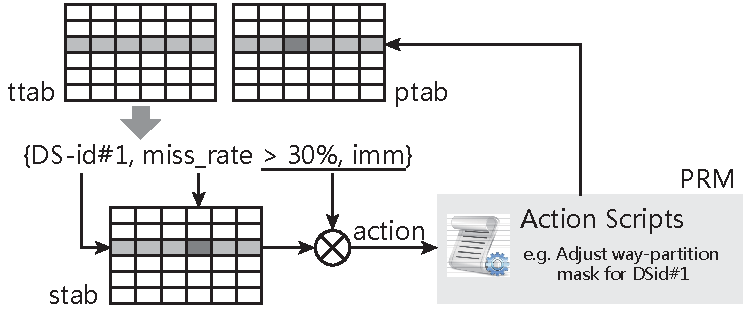
\includegraphics[width=0.7\textwidth]{hwres/trigger-action-flow}
  \caption{``\emph{trigger$\Rightarrow$action}''编程方法示意图}
  \label{fig:trigger-action-flow}
\end{figure}

如图\ref{fig:trigger-action-flow}所示,trigger是基于状态表中某一统计信息(如IPC、缺失率、延迟等)的触发条件,
action是对针对该触发条件所执行的动作,因此action也可以被称为trigger-handler。
触发条件保存在控制平面的触发表中,而与之对应的action动作则是由系统管理员编写,并存储在PRM的固件中。
系统管理员可以为每个应用标签设定不同的``\emph{trigger$\Rightarrow$action}''规则,
以实现不同的资源管理策略。

由于action动作是运行在PRM固件内,因此可以使用任何语言来编写,
并通过PRM提供的方法将其与触发条件建立关联,并在触发条件满足时自动调用。
同时,由于PRM可以控制系统内所有的控制平面,trigger和action可以针对不同的硬件资源进行设定。
例如,可以设定监控访存带宽的触发条件,但它的触发动作却是调整共享末级缓存的容量,
以此影响其命中率,进而实现访存带宽的调整。
通过这种跨硬件资源的触发规则,可以实现更为灵活的节点内硬件资源协同管理。

根据应用的需求为每个应用编写适当的触发规则是十分复杂的工作,
数据中心管理员可以根据不同的资源管理策略,
预定义多种不同的``\emph{trigger$\Rightarrow$action}''触发规则与动作,
并依此为用户提供不同级别的SLA(Service-Level Agreements)。
用户根据自己的QoS需求选择合适的SLA,通过这些预定义的触发规则与动作来满足其QoS需求。

%本节所描述的``\emph{trigger$\Rightarrow$action}''编程方法与上一节所描述的资源监控与管理的编程接口
%将在第\ref{chap:prm}中进行统一介绍。

\subsection{通用控制平面微体系结构设计}
\label{chap:hwresman:cp:uarch}

综合以上控制平面功能与设计,其微体系结构如图\ref{fig:pard-cp-design}所示。
PARD控制平面的核心是3个控制表,即参数表、状态表和触发表。
参数表与硬件模块之间通过参数接口(HW PARAM IF)进行交互,
硬件在收到请求后,使用请求中的应用标签DS-id查询参数表,获取需要的参数;
状态表与硬件模块之间通过状态接口(HW STAT IF)进行交互,
硬件在完成每一个请求后,通过该接口实现状态的更新。
除此之外,控制平面中还包含连接控制平面网络的接口模块,
PRM通过该模块来访问3个控制表。

这3个控制表都使用CAM+RAM的结构实现,
其中参数表与状态表的CAM中使用应用标签DS-id进行索引,
触发表的CAM中除应用标签DS-id外还包括触发条件对应的统计信息编码。
参数表在收到参数查询请求后,通过CAM查询该请求所对应的表项,
并在RAM中获取其参数并返回给硬件模块;
状态表的更新过程与参数表类似,通过CAM查询表项,将新的统计信息更新到RAM对应的表项中;
在状态表更新的同时,应用标签和统计信息编码同样被送到触发表的CAM中,
用于查询是否存在与本次更新相对的触发条件,如果触发条件存在且满足,
则通过CPN接口模块向PRM发送触发事件通知。

\begin{figure}[tb]
  \centering
  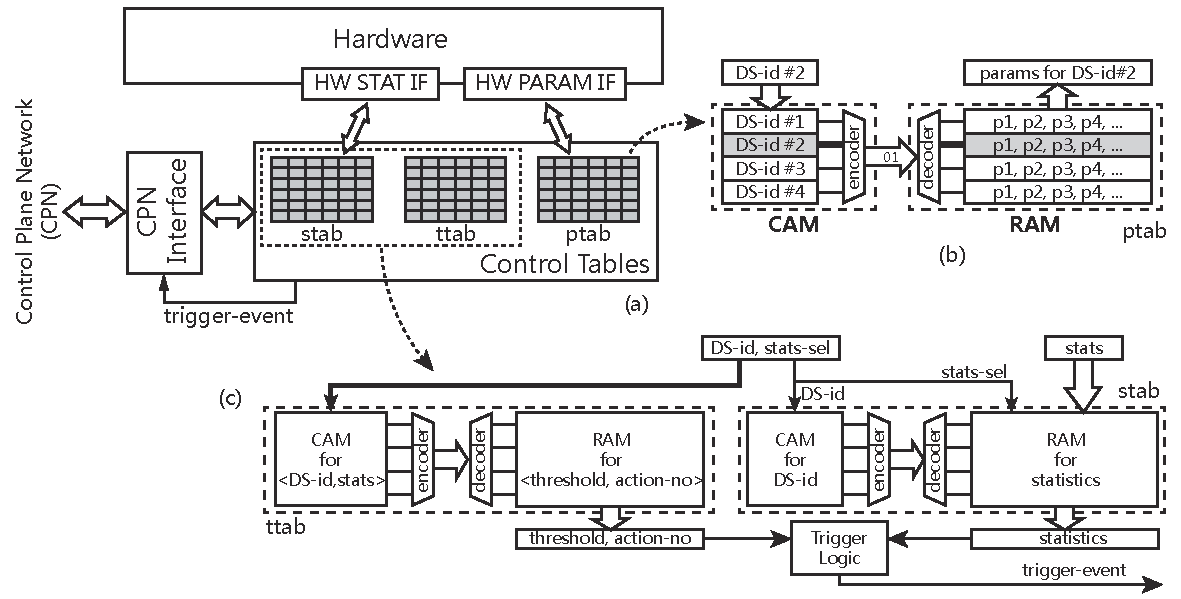
\includegraphics[width=\textwidth]{hwres/pard-cp-design}
  \caption[控制平面微体系结构设计]{控制平面微体系结构设计:
  (a)控制平面的核心是3个控制表,即参数表ptab、状态表stab和触发表ttab,
       以及这3个控制表与控制平面网络和硬件设备的接口模块;
  (b)参数表由CAM和RAM组成,实现按DS-id索引参数的功能;
  (c)状态表与触发表同样由CAM和RAM组成,触发表的CAM按<DS-id, stats>组合索引,
       该图为状态表更新以及触发检查逻辑。}
  \label{fig:pard-cp-design}
\end{figure}

控制平面网络接口模块使用寄存器窗口的方式对外提供控制表的访问,
如图\ref{fig:pard-cp-intf}所示。
系统内所有的控制平面都被映射到一段连续的16位I/O地址空间中(64KB),
每个控制平面在其中使用32个字节用于映射其控制寄存器,控制寄存器的定义如图\ref{fig:pard-cp-intf}所示。
其中IDENT和IDENT\_HIGH 2个寄存器(总计12字节)存储该控制平面的名字,
type寄存器表示该控制平面的类型,
address/cmd/data 3个寄存器用于实现对控制平面中控制表的访问。
其中address寄存器包含逻辑域标签DS-id(16b)、控制表选择(2b)、以及列偏移(14b),
通过该寄存器实现对控制表项的寻址,而cmd寄存器用于指定对该控制表项的操作,
当前的实现中只包含读、写2种类型的操作。
对于写操作,用户需要提前将数据写入到data寄存器,而对于读操作data寄存器的写入操作由控制平面硬件完成,
用户可以从该寄存器中读取所选择的控制表项内容。

PRM通过以上描述的寄存器接口实现对控制平面的编程,具体流程如下:
控制平面驱动首先将目标表项的地址写入到地址寄存器,其中包括逻辑域标签DS-id(行)以及表项偏移(列)。
如果用户的操作是修改表项,则驱动首先将新的表项写入到data寄存器,然后在命令寄存器中写入WRITE命令;
如果是对表项的查询操作,则直接向命令寄存器写入READ命令,并在操作完成后从data寄存器中读取数据。

\begin{figure}[tb]
  \centering
  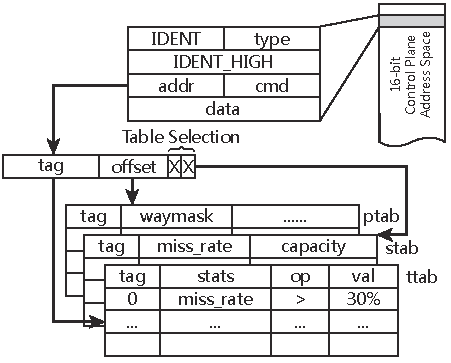
\includegraphics[width=0.5\textwidth]{hwres/pard-cp-intf}
  \caption[控制平面接口]{控制平面接口}
  \label{fig:pard-cp-intf}
\end{figure}


\subsection{控制平面示例}

本节将以处理器末级缓存和内存控制器为例,介绍如何将控制平面集成到硬件部件中,
图\ref{fig:pard-cache-cpdesign}和图\ref{fig:pard-mig-cpdesign}
是已经增加了控制平面的微体系结构示意图。
从中发现,其控制平面具有相同的结构,只是控制表的内容存在差别,
该通用的控制平面结构可以很容易的集成到不同的硬件部件中,
只需要对其控制表及硬件接口部分进行修改。

\textbf{共享末级缓存控制平面}\quad
图\ref{fig:pard-cache-cpdesign}是共享末级缓存控制平面的微体系结构示意图,
其支持可编程的路划分机制,借助该机制可以为应用程序调整Cache容量。
其控制平面由3个基本的控制表组成,并通过可编程接口由PRM中运行的固件访问;
控制平面同时还包括1个连接到PRM的中断线,用于发送触发逻辑产生的中断通知。
除了引入控制平面以外,还需要对原有缓存控制器中的Tag Array以及伪LRU逻辑进行修改,
所有这些修改均以阴影和虚线的方式在图中进行了标识。

\begin{figure}[tb]
  \centering
  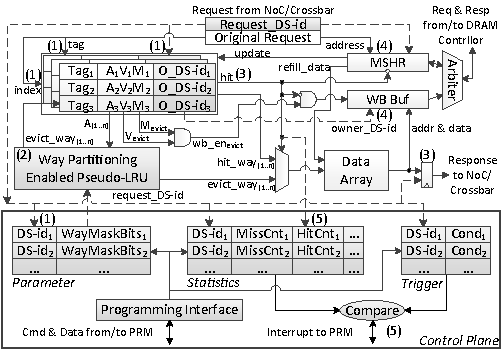
\includegraphics[width=0.7\textwidth]{hwres/pard-cache-cpdesign}
  \caption{共享末级缓存控制平面}
  \label{fig:pard-cache-cpdesign}
\end{figure}

控制平面的引入是否会为共享末级缓存带来额外的延迟是在设计过程中需要考虑的重要问题,
幸运的是目前系统中Cache控制器都是基于流水线设计,
这就使得控制平面的逻辑开销能够隐藏在原有的流水线中,具体流程如下:

\begin{enumerate}[leftmargin=2\parindent, nolistsep, label=(\arabic*)]
  \item 当包含DS-id和地址的Cache访问请求到达控制器时,
        首先需要利用DS-id从参数表中获得相应的路划分掩码。
        例如掩码``0x00FF''代表在整个16路中仅使用低端的8路。
        与此同时,请求地址被用来在Tag Array中查找相应的条目,
        这些条目除了普通的Tag和状态信息以外,还保存有DS-id;
  \item 伪LRU逻辑利用参数表输出的掩码以及Tag Array输出的访问历史计算出需要被替换的路(victim);
  \item 如果请求在缓存中命中,那么数据将从Data Array中取回,
        连同请求的DS-id一起通过NoC或者crossbar返回给CPU。
        需要注意的是,缓存的命中条件发生了改变,除了请求地址与条目Tag之间原有的约束以外,
        还需要请求DS-id与条目DS-id相互匹配。
  \item 如果请求在缓存中没有命中,Cache控制器会分配1个MSHR条目,
        并在该条目中保存原始请求及其DS-id。
        当被请求的数据返回时,Cache控制器需要将MSHR中保存的原始请求DS-id写入到TagArray中。
        该DS-id作为``owner DS-id'',在脏数据写回时,
        需要与地址和数据一同送入回写缓存,并发送到内存控制器。
  \item 在以上各个步骤的过程中,Cache控制平面还会完成以下若干操作:
        更新统计表,将Cache使用统计数据发送给平台资源管理器,
        在必要时激活触发条件并发出中断信号给PRM。
        需要特别指出的是这些操作并不在关键路径上,不会对延迟造成影响。
\end{enumerate}

%可编程接口用于PRM固件访问该控制平面的3个控制表,
%它首先从PRM接收控制表的访问命令,选择相应的表并从指定的表项中读取或写入数据,
%更多细节请参见第\ref{chap:prm}章。

\textbf{内存控制器控制平面}\quad
图\ref{fig:pard-mig-cpdesign}是内存控制器控制平面的微体系结构示意图,
为了让PARD的逻辑域抽象能够运行未经修改的操作系统和应用,
该控制平面的参数表保存了用于逻辑域物理地址与DRAM地址的映射信息。
除此之外,控制表中还保存了每个逻辑域的优先级信息用于访存调度。

\begin{figure}[tb]
  \centering
  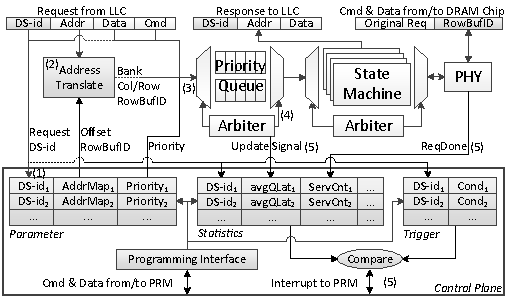
\includegraphics[width=0.7\textwidth]{hwres/pard-mig-cpdesign}
  \caption{内存控制器控制平面}
  \label{fig:pard-mig-cpdesign}
\end{figure}

在性能隔离方面,与Cache控制面不同的是内存控制器控制平面需要考虑以下2个因素:
排队延迟和行缓冲(row buffer)局部性。
为了管理排队延迟,PARD在内存控制器中加入了优先级队列机制,
队列数目取决于内存控制平面能够支持的优先级等级。
当前的设计中暂时仅支持2个优先级,该设计可以很容易的扩展到多个优先级。
为了防止低优先级访存请求干扰并降低高优先级访存请求的行缓冲命中率,
在DRAM芯片中为高优先级内存请求增加了1个额外的专用行缓冲。
如果需要为DRAM芯片增加更多的优先级控制能力,
可以参考NEC的virtual-channel memory(VCM)\cite{nec-vcm}技术。

在添加了以上机制后,当附带应用标签的访存访请求到达内存控制器后,
将会顺序引发下列操作:

\begin{enumerate}[leftmargin=2\parindent, nolistsep, label=(\arabic*)]
  \item 控制平面利用请求的DS-id从参数表中获得与之相应的地址映射信息、
        队列优先级以及行缓冲编号;
  \item 将请求中的逻辑域物理地址转换成DRAM物理地址;
  \item 根据控制表中获取的优先级信息将请求连同DS-id置入相应的请求等待队列中;
  \item DRAM调度器根据高优先级优先以及FR-FCFS\cite{rixner_memory_2000}策略从等待队列中选取请求进行服务;
  \item 控制平面更新统计表并检查是否满足触发条件,如果满足则发送中断信号到PRM。
\end{enumerate}


\subsection{基于PARD模拟器的评测}

本节在第\ref{chap:labeladdrspace:nohype}节所建立的模拟器基础上,
按照本章所述方法对处理器末级缓存、内存控制器和磁盘控制器进行改造,包括:
1)在处理器末级缓存中增加缓存容量划分功能;
2)在内存控制器中增加控制平面,实现地址映射;
3)在磁盘控制器中增加基于带宽划分的调度功能。
并为它们增加控制平面,同时在模拟器中模拟了基于X86-SoC的PRM,
实现对这2个硬件资源的集中式管理。
表\ref{tab:pard-sim-cp}给出了3个控制平面中控制表的设计。

缓存容量划分选择了最简单的按路划分的方式,控制平面提供路划分掩码,
修改Cache替换策略,按照控制平面所提供的掩码进行替换目标的选择,实现路划分。
对于磁盘带宽划分,使用基于时间片的调度方法,即通过划分固定时间间隔的时间片,
设置在该时间片内所允许的最大带宽,实现对带宽的划分。

修改后的模拟器最多支持启动4个逻辑域,
能够通过PRM调整4个逻辑域对处理器末级缓存与磁盘控制器的资源分配,
本节将使用该模拟器验证控制平面对资源分配的控制(磁盘控制器)、
以及``\emph{trigger$\Rightarrow$action}''机制的效果(处理器末级缓存)。

\begin{table}[ht]
  \centering
  \begin{minipage}[t]{0.9\linewidth}
  \caption{PARD模拟器控制平面控制表设计}
  \label{tab:pard-sim-cp}
    \begin{tabular*}{\linewidth}{p{0.15\textwidth}<{\centering}lll}
      \toprule[1.5pt]
             & \textbf{Parameter Table} & \textbf{Statistics Table} & \textbf{Trigger Table} \\
      \midrule[1pt]
       Cache & way mask-bits            & miss rate, capacity       & miss rate $\Rightarrow$ way mask-bits \\
      Memory & address mapping          & bandwidth, latency        & \emph{N/A}         \\
        Disk & bandwidth quota          & bandwidth                 & \emph{N/A}         \\
      \bottomrule[1.5pt]
    \end{tabular*}\\[2pt]
  \end{minipage}
\end{table}



\subsubsection{``\emph{trigger$\Rightarrow$action}''机制验证}

本节利用``\emph{trigger$\Rightarrow$action}''机制解决应用服务质量与服务器资源利用率冲突的问题,
实验场景与配置如图\ref{fig:hwres-sim-config}所示:
1台四核的PARD服务器被划分为4个逻辑域,其中LDom\#0中运行延迟敏感型应用memcached,
另外3个逻辑域中运行批处理应用,考察资源共享对延迟敏感型应用性能的影响。

由于模拟器本身的模拟速度非常慢,增加网络环境模拟会进一步降低模拟速度,
因此在实验时将memcached服务器与客户端运行在同一个逻辑域中,它们共享一个CPU核心。
虽然服务器和客户端会在逻辑域内发生资源竞争,
但由于本文更多关注的是逻辑域(应用)之间的干扰,这种黑箱内部的竞争是可接受的。
本实验使用STREAM benchmark\cite{stream}作为批处理应用,
该benchmark会在处理器末级缓存产生严重的干扰,另实验效果更加明显。

实验分为2步,
首先使用模拟器的simple-timing模型来启动Linux操作,启动应用并建立checkpoint;
然后使用Out-of-Order(O3)模型恢复该checkpoint,最后的实验评估使用O3模型进行。
受到模拟速度的影响,本实验只模拟了memcached应用的3秒钟执行(花费大约30个小时),
其中第1秒是warm-up过程,后2秒才被用于评估。

\begin{figure}[tb]
  \centering
  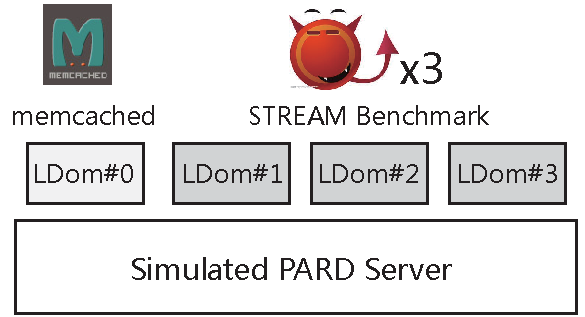
\includegraphics[width=0.5\textwidth]{hwres/hwres-sim-config}
  \caption{``\emph{trigger$\Rightarrow$action}''机制验证实验配置}
  \label{fig:hwres-sim-config}
\end{figure}

\begin{figure}[b]
\begin{minipage}{0.48\textwidth}
  \centering
  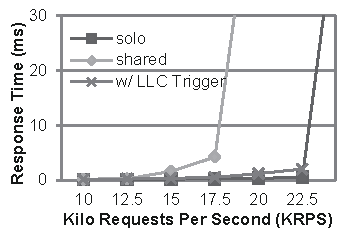
\includegraphics[height=4.5cm]{hwres/pard-sim-memcached-resptime}
  \caption{模拟器memcached 95\%-tail延迟示意图}
  \label{fig:pardsim:memcached-resptime}
\end{minipage}\hfill
\begin{minipage}{0.48\textwidth}
  \centering
  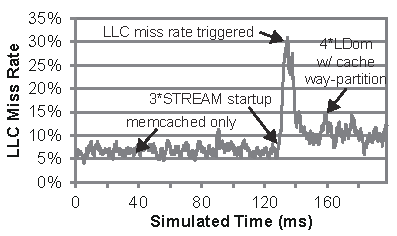
\includegraphics[height=4.5cm]{hwres/pard-sim-memcached-20krps-missrate}
  \caption{模拟器memcached末级缓存命中率变化(20KRPS)}
  \label{fig:pardsim:memcached-20krps-missrate}
\end{minipage}
\end{figure}


图\ref{fig:pardsim:memcached-resptime}展示了在不同请求负载下memcached的长尾响应时间。
当memcached单独运行时(图中solo曲线),它能够满足22.5KRPS的请求负载,
同时长尾(95\%-tail)响应时间在合理的范围(0.6ms)。
然而,由于只1个处理器核在运行,此时服务器的利用率仅为25\%。
如果另外3个逻辑域也被启动运行,并与memcached所在的逻辑域共享资源,
整个服务器达到100\%的利用率,
但此时memcached的性能下降到17.5KRPS,并且长尾响应时间也超过了1ms。
如果进一步提高请求负载到20KRPS,长尾响应时间增加超过2个数量级(62.6ms)。

为了验证``\emph{trigger$\Rightarrow$action}''机制的效果,
预先在PRM中为memcached所在的逻辑域LDom\#0定义了与图\ref{fig:trigger-action-flow}
类似的触发规则:
\begin{verse}
``\emph{LLC.MissRate $>$ 30\% $\Rightarrow$ 增加LLC容量到全部容量的50\%}''
\end{verse}

在启动所有的逻辑域前,将以上规则安装到处理器末级缓存控制平面中,
图\ref{fig:pardsim:memcached-20krps-missrate}给出了实验过程中收集的处理器末级缓存缺失率,
从图中可以看到当3个干扰应用运行后,memcached的缓存缺失率显示上升,
并达到了规则设定的触发阈值(30\%),控制平面应用action动作,
将一半的缓存容量划分给memcached所在的逻辑域,在此之后memcached的缓存缺失率显著下降,
降低到10\%左右,只略高于单独运行时7\%的缺失率。
最终在22.5KRPS的请求速率下,长尾响应时间只有1.2ms,
由于memcached所能使用的处理器末级缓存只有单独运行时的一半,
因此其长尾响应时间要略高于单独运行时的响应时间。

以上实验结果表明,即使4个处理器核全部都在工作,服务器资源利用率为100\%的情况下,
memcached的性能仍然没有受到严重的影响。
这证明``\emph{trigger$\Rightarrow$action}''机制能够利用PARD提供的硬件资源管理功能,
实现服务器资源利用率与应用服务之间的平衡。


\subsubsection{磁盘I/O带宽控制}

PARD控制平面不仅能管理处理器末端级缓存这类基于容量的资源,
同时能够管理基于流量的资源,如内存带宽与I/O带宽。
本节验证控制平面对带宽的控制,这里使用磁盘I/O带宽作为实验目标。

在本节的实验中,只使用模拟器中2个逻辑域,在其中使用命令
``\textit{dd if=/dev/zero of=/dev/sdb bs=}32\textit{M count=}16''
执行磁盘写操作。
初始状态下,2个逻辑域共享磁盘控制器且具有相同的优先级,由于它们执行的命令与参数完全相同,
因此2个逻辑域所得到的磁盘I/O带宽完全相同。
此时假设逻辑域LDom\#0的用户需要得到更好的I/O性能,例如云计算场景下通过更高的费用获取更快的性能,
管理员可以在PRM内执行以下命令重新调整服务器中磁盘I/O带宽的分配,将80\%的带宽分配给该用户。
\begin{verse}
\textit{echo} 80 \textit{$>$ /sys/cpa/cpa}3\textit{/ldom}0\textit{/parameters/bandwidth}
\end{verse}

该命令通过PRM对磁盘控制器控制平面(cpa3)进行编程,修改LDom\#0的带宽占比为80\%,
图\ref{fig:pardsim:iosched}给出了磁盘I/O带宽分配的效果。

\begin{figure}[b]
  \centering
  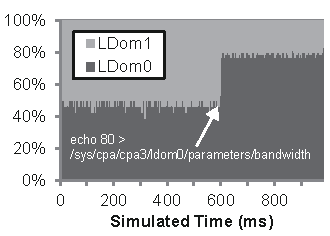
\includegraphics[width=0.45\textwidth]{hwres/pard-sim-iosched}
  \caption{磁盘I/O性能隔离}
  \label{fig:pardsim:iosched}
\end{figure}


虽然诸如cgroup\cite{cgroup}之类的方法也能提供类似的I/O带宽管理功能,
但PARD所提供的资源管理方法能够在硬件层次实现更为细粒度的资源管理,
同时无需对用户操作系统或应用进行任何的修改,降低了软件栈的复杂度与开销。
关于控制平面的编程接口,以及如何在PRM中实现资源管理将在第\ref{chap:prm}章进行详细的介绍。


\section{可编程数据平面设计}
\label{chap:hwresman:dp}

正如本章引言所述,PARD的硬件资源管理机制包括控制平面与数据平面2部分,
上节已经介绍了控制平面的设计,
本节主要针对数据平面的需求设计可编程数据平面,具体包括:
数据平面处理器的设计、资源管理机制的集成、以及数据平面可编程的实现。
由于数据平面中包含额外的数据平面处理器,使得整个模拟器模拟速度进一步变慢,
因此本节将不使用模拟器对数据平面的功能与开销进行验证,
而直接在第\ref{chap:impl}章使用FPGA原型系统进行验证。

%需要能够适应不同的硬件,并为控制平面提供统一的管理接口;
%能够提供灵活的可编程机制;
%能够很容易的集成现有资源管理相关工作。
%
%可编程技术目前主要包括2类,一类是以FPGA为代表的硬件可编程,一类是使用处理器实现软件。
%
%基于xxxx的考虑,本文使用基于处理器的实现。
%
%另一方面,控制平面的``\emph{trigger$\Rightarrow$action}''机制在响应时间上存在瓶颈:
%每当触发条件发生后,需要经过控制平面网络将该事件传递到PRM,
%由运行在PRM中的软件代码来更新策略,并通过控制平面网络写回到控制平面中。
%由于受到控制平面网络延迟以及PRM软件代码延迟的影响,
%该机制并不能达到特别高的响应速度。
%同时并非所有的触发条件发生后都需要在PRM进行全局处理,
%完全可以预定义一些动作,在控制平面本地完成处理。
%
%本节后续内容将对数据平面处理器的设计以及资源管理机制的集成进行介绍,
%最后介绍数据平面运行时可编程的实现。

\subsection{数据平面处理器体系结构}

\begin{figure}[tb]
  \centering
  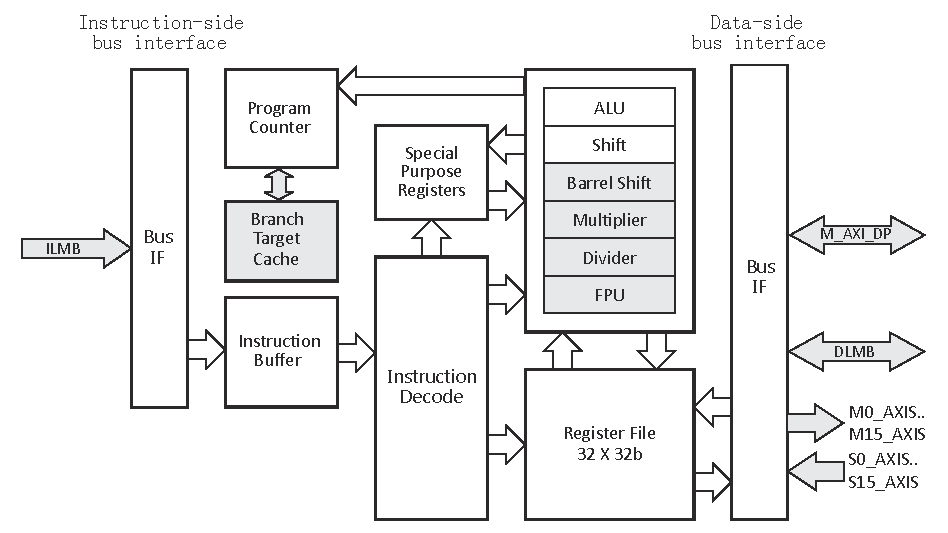
\includegraphics[width=0.8\textwidth]{hwres/pard-dp-proc}
  \caption{数据平面处理器结构图}
  \label{fig:pard-dp-proc}
\end{figure}

由于数据平面处理器位于请求处理的关键路径上,为了保障系统的性能不受影响,需要从以下3个方面进行考虑:

\begin{enumerate}[leftmargin=2\parindent, nolistsep, label=\arabic*)]
  \item 处理器需要执行一系列指令才能完成对请求的处理,因此处理器需要工作在比其所在硬件部件更高频率,以满足硬件部件的性能需求;
  \item 处理器的固件代码执行需要确定性,因此不能使用cache结构,而是使用scratchpad memory代替;
  \item 由于高频率的需求,因此处理器功能要尽可能简单,一些复杂逻辑(如数据压缩与加密等)通过外部加速器的方式进行扩展。
\end{enumerate}

基于以上需求,本文最终选择使用RISC作为数据平面处理器的基础架构,并对其进行修改以适应数据平面处理器的需求,如图\ref{fig:pard-dp-proc}所示。
包括:1)架构精简,只保留其基本功能,以满足频率需求;
2)增加scratchpad memory作为指令与数据存储;
3)增加请求缓存接口用于接入硬件设备;
4)增加控制平面接口用于接入控制平面。
由第\ref{chap:hwresman:res}节可知,对于内存控制器与处理器末级缓存,该处理器的主要工作包括:
对请求进行调度、地址变换,对数据进行处理,生成控制信号(如Cache缓存与替换)。
要完成以上工作,该处理器需要具备基本的处理器功能外,还需要在数据类型、存储模型和指令上进行扩展。

\subsubsection{数据类型}

数据平面处理器中执行的算法代码大都只是对输入的请求进行处理,
因此该处理器只有``无符号整数''和``请求'' 2种数据类型,如图\ref{fig:pard-dp-datatype}所示。
无符号整数的长度与处理器的位宽相同,都被设置为其所属硬件的位宽,
以节约请求处理时位宽转换的开销,保障请求处理的效率。

``请求''类型的是变长数据类型,其中包含了固定16b长度的应用标签(DS-id)以及变长的请求数据。
以访存请求为例,其中包含请求地址、长度、线程号、读写类型、锁与缓存状态等其他标志位;
对于Cache替换请求,其中包含了请求地址、Hit/Miss标记以及其他标志位信息。
图\ref{fig:pard-dp-datatype}给出了访存请求以及Cache替换请求类型的示例。
数据平面处理器本身并不关心请求类型中具体每个位的意义,而只是将其做为整体进行处理,
对每个域的解析或修改由其运行的固件代码完成。

\begin{figure}[hb]
  \centering
  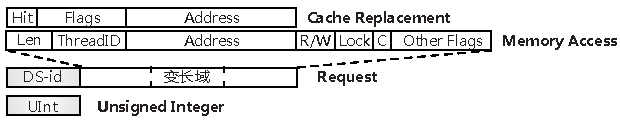
\includegraphics[width=0.7\textwidth]{hwres/pard-dp-datatype}
  \caption{数据平面处理器支持的数据类型}
  \label{fig:pard-dp-datatype}
\end{figure}
 
\subsubsection{存储模型}
数据平面处理器中程序员可见的存储结构包含寄存器、请求缓存、scratchpad memory、I/O地址空间四部分。
与传统的RISC架构相同,数据平面处理器包含32个通用寄存器($r0\sim r31$),
用于进行算数逻辑运算,其中$r0$是常数0;
除此之外,增加4个用于保存``请求''类型数据的请求寄存器($s0\sim s3$),
可以通过请求缓存操作指令(rbget和rbput,参见第\ref{chap:hwresman:dp:isa}节),
将请求输入队列中的请求读取到该寄存器、或将该寄存器中的请求加入到请求输出队列中;
请求寄存器不能直接参与算术逻辑计算,需要先将其部分数据读取到通用寄存器后才能执行计算;
请求寄存器之间可以直接进行数据交换。
处理器执行的固件代码与数据保存在scratchpad memory中,需要用户自行管理。
控制平面被映射为数据平面处理器的外设,提供处理器的固件代码ROM以及处理器的对外接口。

\subsubsection{指令集}
\label{chap:hwresman:dp:isa}

数据平面处理器使用RISC标准的算数逻辑、控制流和访存指令,
并在其基础上额外增加了请求缓存操作指令。

请求缓存分为输入缓存和输出缓存2部分。
其中输入缓存既可作为FIFO操作,也可基于DS-id进行内容寻址;
输出缓存只能作为FIFO操作。
用于请求缓存操作的指令如表\ref{tab:pard-dp-isa}所示,
指令rbput可以将指定请求寄存器中的请求添加到输出缓存队列末尾;
指令rbget有2种使用方式,一种是将输入缓存作为FIFO,取出队列头的请求到请求寄存器,
另一种是通过DS-id对请求进行筛选,取出第1个满足应用标签的请求到请求寄存器。
指令rbcp用于在请求寄存器之间传送数据。
指令mfrb用于将请求寄存器中的部分数据传送到通用寄存器;
指令mtrb与之相反,用于将通用寄存器的数据传送到请求寄存器指定的位置。

% 数据平面处理器扩展指令
\begin{table}[htb]
  \centering
  \begin{minipage}[t]{0.95\linewidth}
  \caption{数据平面处理器扩展指令}
  \label{tab:pard-dp-isa}
    \begin{tabular*}{\linewidth}{p{0.12\textwidth}<{\centering}ll}
      \toprule[1.5pt]
      {\heiti 指令} & {\heiti 用途} \\
      \midrule[1pt]

      \multirow{2}{*}{\textbf{rbput}} & \multicolumn{2}{l}{将请求寄存器中的请求增加到请输出请求缓存FIFO队尾。示例:}                               \\
                                      & rbput \textit{rb}0, \textit{s}0 & \#将\textit{s}0加入到\textit{rb}0队尾                                    \\
      \hline
      \multirow{3}{*}{\textbf{rbget}} & \multicolumn{2}{l}{从输入请求缓存读取一个请求到指定的请求寄存器。示例:}                                   \\
                                      & rbget \textit{s}0, \textit{rb}0                & \#从\textit{rb}0获得第1个请求到\textit{s}0寄存器          \\
                                      & rbget \textit{s}0, \textit{rb}0, \textit{DSid} & \#从\textit{rb}0获得第1个\textit{DSid}为给定值的请求到\textit{s}0寄存器 \\
      \hline
      \multirow{2}{*}{\textbf{rbcp}}  & \multicolumn{2}{l}{请求缓存寄存器之间传递数据}                                                             \\
                                      & rbcp \textit{s}0, \textit{s}1                  & \#将\textit{s}1的值传递给\textit{s}0                      \\
      \hline
      \multirow{3}{*}{\textbf{mfrb,mtrb}}   & \multicolumn{2}{l}{请求缓存寄存器与通用寄存器之间传递值。示例:}                                     \\
                                      & mfrb \textit{r}4, \textit{s}0, 0               & \#将\textit{s}0第1个32位数据送到\textit{r}4寄存器         \\
                                      & mtrb \textit{s}1, \textit{r}5, 1               & \#将\textit{r}5寄存的数据送到\textit{s}1寄存器第2个32位   \\
      \bottomrule[1.5pt]
    \end{tabular*}\\[2pt]
  \end{minipage}
\end{table}

\subsection{固件代码示例}
本节将以3段不同功能的固件代码为例,介绍数据平面处理器的编程方法。

\begin{figure}[H]
  \centering
  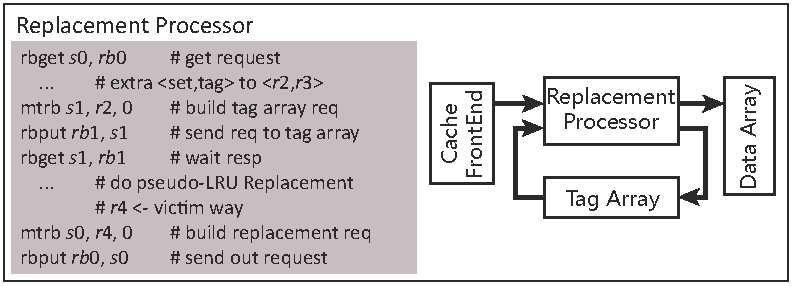
\includegraphics[width=0.7\textwidth]{hwres/pard-dp-ex-cache}
  \caption{缓存替换策略示例}
  \label{fig:pard-dp-ex-cache}
\end{figure}

\textbf{缓存替换策略}\quad
本示例实现缓存替换策略功能,使用可编程处理器替换Cache中原有的LRU模块,
使用软件实现基于二叉树的伪LRU替换策略。
如图\ref{fig:pard-dp-ex-cache}所示,处理器固件代码工作流程如下:
1)处理器收到Cache前端的请求后,以及Hit/Miss信息,如果缓存命中则无需任何额外操作;
2)对于缓存缺失的请求,首先从地址中解析出tag与set信息,
并将解析后的set地址发送到Tag Array,等待其返回该set的信息;
3)根据TagArrary返回的set信息,以及内部的数据结构生成替换目标;
4)将替换目标送出处理器。

\textbf{段式地址映射}\quad
本示例用于实现PARD的内存控制器控制平面所提供的地址映射功能,
该功能只需要对访存请求的地址进行修改,而请求的数据无需修改,
因此将地址与数据分开由2个处理器进行处理,
如图\ref{fig:pard-dp-ex-mapping}所示。
对于数据处理器,其固件代码只使用rbget/rbput指令对请求进行转发。
地址处理器首先需要使用rbget指令获取当前请求到请求寄存器,
并使用mfrb指令将其中的地址与DSid读取到通用寄存器;
而后通过查表的方式获得该请求对应的映射目的地址的基址,
对请求地址进行变换,并使用mtrb指令将变换后的地址写回到请求寄存器,
最后通过rbput指令将新的访存请求从处理器中送出,完成地址映射功能。

\begin{figure}[H]
  \centering
  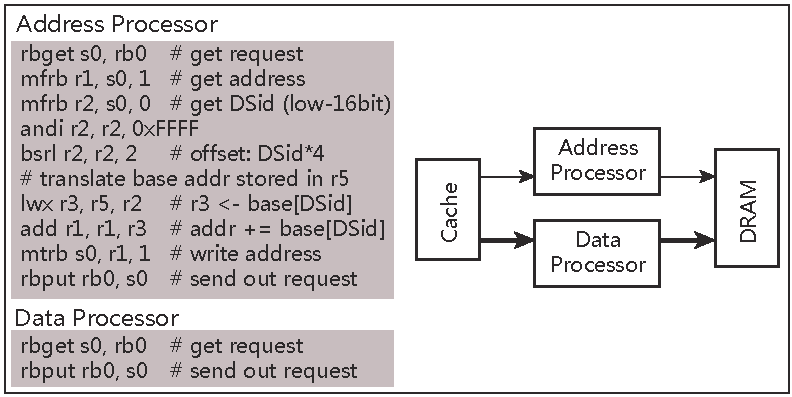
\includegraphics[width=0.7\textwidth]{hwres/pard-dp-ex-mapping}
  \caption{段式地址映射示例}
  \label{fig:pard-dp-ex-mapping}
\end{figure}
 
\textbf{数据加密}\quad
本示例实现访存数据加密功能,由于数据加密操作通常需要耗费很长的时间,
而且数据平面处理器提供的指令集并不足以完成该操作。
因此在处理器外部实现了硬件AES加密模块,并通过请求接口将其连接到数据平面处理器上,
该结构如图\ref{fig:pard-dp-ex-aes}所示。
基于该结构,数据处理器只需要将数据发送到AES模块并等待其完成加密,
将加密后的数据送出处理器即可。
数据解密与加密过程类似,只需将数据发送到连接有解密模块的请求接口即可。

\begin{figure}[H]
  \centering
  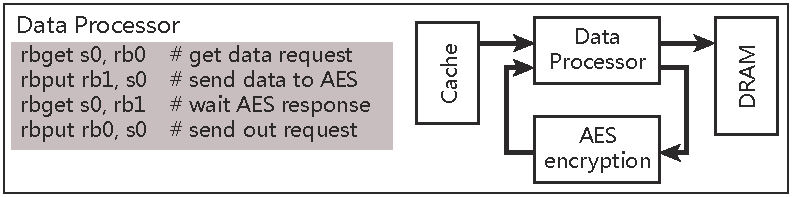
\includegraphics[width=0.7\textwidth]{hwres/pard-dp-ex-aes}
  \caption{访存数据加密示例}
  \label{fig:pard-dp-ex-aes}
\end{figure}
 

\subsection{可编程支持}

数据平面的可编程主要体现在数据平面处理器的固件代码更新,
通过更新固件代码的方式实现策略的调整。
对数据平面处理器固件代码更新可以分为兼容性更新与非兼容性更新,
其中``兼容性''是指更新前后的代码是否对数据平面的功能产生更改。
对于非兼容性更新,需要首先关闭系统中所有正在运行的逻辑域,
并在数据平面处理器固件更新完成后重新启动逻辑域;
对于兼容性更新,系统可实现无中断运行,
但需要对数据平面处理器与硬件的接口处进行额外的处理,
如图\ref{fig:pard-dp-fw-upgrade}所示。

在收到更新固件命令后进入Drain状态,阻止请求继续发送到数据平面处理器,
等待数据平面处理器处理完全部请求,并将请求队列排空后,使处理器进入Isolated隔离状态;
之后完成对固件代码的更新,新的固件代码开始运行后,开始进行初始化操作,
其中包括旧固件的状态数据迁移步骤;
在所有的初始化操作完成后,处理器恢复到就绪状态,重新开始处理请求,
至此完成数据平面处理器固件代码的兼容性更新操作。

\begin{figure}[htb]
  \centering
  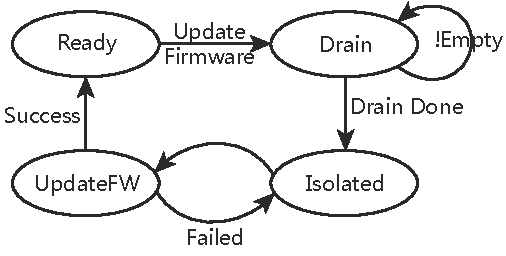
\includegraphics[width=0.6\textwidth]{hwres/pard-dp-fw-upgrade}
  \caption{数据平面处理器兼容性固件更新状态图}
  \label{fig:pard-dp-fw-upgrade}
\end{figure}


\section{小结}

本章介绍了PARD体系结构中硬件资源共享管理方法与架构,
包括硬件资源的``数据平面''与``控制平面''抽象,及其具体的实现。
控制平面通过控制表实现,为用户提供了资源管理接口,
同时提出了``\emph{trigger$\Rightarrow$action}''编程方法,
基于模拟器的实验结果表明,该方法与PARD提供的资源管理机制结合,
能够实现数据中心服务器资源利用率与应用服务质量的平衡。
针对数据平面可编程需求,本章提出数据平面处理器设计,
并将其应用到处理器末级缓存与内存控制器数据平面中,
通过软件编程的方式实现硬件资源管理的扩展。



%%% Local Variables:
%%% mode: latex
%%% TeX-master: t
%%% End:

\chapter{共享资源协同管理}
\label{chap:prm}

应用负载具有波动性,对硬件资源的需求会发生变化,需要提供一种动态调整应用资源分配的方案。

有三个层次,分别:
(1)节点内不同硬件资源的协同管理;
(2)节点内应用调度与资源协同管理;
(3)节点间协同管理;


PRM软件接口,

- 与mesos集成,实现硬件支持的容器

- 与OpenStack集成,实现IaaS平台

- 与SDN集成,实现网络中心的系统

\begin{figure}[tbh]
  \centering
  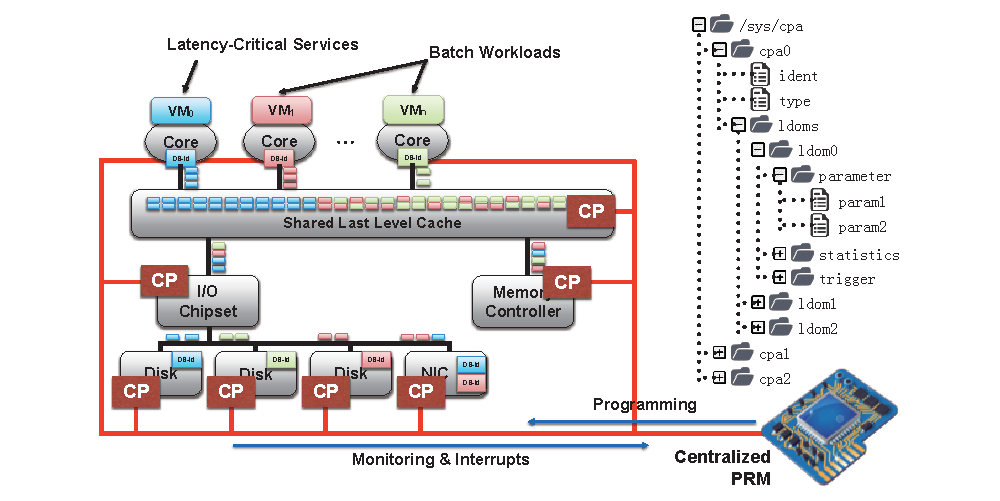
\includegraphics{arch/pard-arch-outline.pdf}
  \caption[PARD体系结构概况]{PARD体系结构概况}
  \label{fig:pard-arch-outline}
\end{figure}



%%% Local Variables:
%%% mode: latex
%%% TeX-master: t
%%% End:

\chapter{PARD原型系统实现与验证}
\label{chap:impl}

基于前四章的设计,本章实现了资源管理可编程体系结构PARD的原型系统,
包括基于gem5的全系统模拟器实现以及Xilinx VC709平台上的FPGA原型。
之前的章节中已经通过模拟器对PARD体系结构的部分功能进行了验证,
本章将着重介绍FPGA原型系统,具体安排如下:
首先对模拟器平台进行介绍,然后介绍FPGA原型系统的设计与实现,
包括整个系统以及控制平面、数据平面的实现,
最后对FPGA原型系统的功能以及开销进行分析。

\section{PARD模拟器}

As shown in Table \ref{tab:pard-sim-setup}
PARD-gem5 is a cycle-accurate simulator that is able to simulate OoO X86 systems.
In particular, we added tag registers in CPU cores,
implemented LLC, memory controller, I/O bridge and
IDE control planes.
Table \ref{tab:pard-sim-cp} illustrates major
content of the three tables of the LLC, memory and IDE control planes.
We also implemented the PRM that is also based on an X86 processor running
at 100MHz, 16MB DRAM, 32MB Flash, one Ethernet adaptor and four control plane adaptors (CPAs).
The firmware running on the PRM is based on a tailored
Linux kernel 2.6.28.4 with Busybox \cite{busybox} toolkit.

With these efforts, PARD-gem5 is able to simulate a PARD server that can
be partitioned into multiple LDoms. Each LDom can run unmodified Gentoo Linux
with kernel 2.6.28.4 and memcached 1.4.17 \cite{memcached} of CloudSuite \cite{Ferdman:2012:cloudsuite} etc.


\begin{table}[ht]
  \centering
  \begin{minipage}[t]{0.9\linewidth}
  \caption{PARD模拟器参数}  
  \label{tab:pard-sim-setup}
    \begin{tabular*}{\linewidth}{rl}
      \toprule[1.5pt]
      CPU                  & 4 4-issue Out-of-Order X86 cores, 2GHz\\
      L1-I/core            & 64KB 2-way, hit = 2 cycles \\
      L1-D/core            & 64KB 2-way, hit = 2 cycles \\
      Shared LLC           & 4MB 16-way, hit = 20 cycles \\
      \hline
      DRAM                 & 8GB DDR3-1600 11-11-11, 4Gbit chip (Micron MT41J512M8) \\
                           & 1 channel, 2 ranks/channel, 8 banks/Rank \\
                           & Burst Length = 8, Row buffer = 1KB \\
                           & tCK=1.25ns, tRCD = 13.75ns, tCL = 13.75ns, tRP = 13.75ns, tRAS = 35ns, \\
                           & tRRD = 6ns \\
      \hline
      Disks                & 4-channel IDE controller, 8 disks \\
      \hline
      Platform             & 100MHz X86 core, 16MB DRAM, 32MB Flash Storage \\
      Resource             & 1 Ethernet adaptor  \\
      Manager              & 4 control plane adaptors (CPA) \\
      (PRM)                & Firmware: tailored Linux kernel 2.6.28.4 with Busybox \cite{busybox} \\
      \hline
      Server OS            & Gentoo Linux with kernel 2.6.28.4 \\
      \hline
      Workloads            & Memcached \cite{memcached}, SPECCPU 2006 \cite{cpu2006} \\
                           & Microbenchmark: CacheFlush \& DiskCopy \\
      \bottomrule[1.5pt]
    \end{tabular*}\\[2pt]
  \end{minipage}
\end{table}

\begin{table}[ht]
  \centering
  \begin{minipage}[t]{0.9\linewidth}
  \caption{PARD模拟器控制平面控制表设计}
  \label{tab:pard-sim-cp}
    \begin{tabular*}{\linewidth}{rl}
      \toprule[1.5pt]
        \textbf{Parameter Table}  &   Cache: way mask-bits                               \\
                                  &   Memory: row-buffer mask-bits, scheduling priority, address mapping \\
                                  &   Disk: bandwidth                                    \\
        \hline
        \textbf{Statistics Table} &   Cache: miss rate, capacity                         \\
                                  &   Memory: bandwidth, latency                         \\
                                  &   Disk: bandwidth                                    \\
        \hline
        \textbf{Trigger Table}    &   LLC miss rate $\Rightarrow$ way mask-bits          \\
                                  &   Memory latency $\Rightarrow$ row-buffer mask-bits  \\
                                  &   Memory latency $\Rightarrow$ scheduling priority   \\
      \bottomrule[1.5pt]
    \end{tabular*}\\[2pt]
  \end{minipage}
\end{table}

\section{FPGA原型系统}

\subsection{基础系统选择}

实现PARD原型系统的第一个工作是选择一个合适的基础系统,
PARD对基础系统有以下需求:

\begin{enumerate}
  \item 能够在FPGA环境下综合;
  \item 独立系统,不依靠任何辅助设施即可运行;
  \item 丰富的I/O设备支持,支持Xilinx VC709开发板所提供的外设,如以太网和PCI-Express;
  \item 能够运行Linux操作系统;
  \item 频率/性能足够运行常见Benchmark应用,如SpecCPU、PARSEC等);
  \item 可以运行典型的数据中心应用,如memcached、httpd等;
  \item 具备完整的软件开发环境;
\end{enumerate}

虽然在开源领域有大量可用的处理器软核,如Oracle OpenSPARC T1\cite{sparct1}、
RISC-V\cite{riscv}、OpenRISC\cite{or1k}、LEON3\cite{leon3}等,
但这些软核并不能满足PARD原型系统的需求。
其中OpenSPARC T1和RISC-V目前的FPGA实现并不是一个独立系统,
需要额外的处理器(如MicroBlaze或ARM)作代理以实现访存与I/O操作;
OpenRISC 1200的软件开发环境支持并不完整;
LEON3是目前开源的处理器软核中最为合适的选择,但其对linux内核的支持并不好,
目前只能运行早期的内核版本,同时软件环境也比较老旧,运行数据中心应用存在一定的困难。
一些FPGA厂商也提供了可配置的处理器核,
如Xilinx的MicroBlaze\cite{microblaze}和ARM\cite{zynq},以及Altera的NIOS II\cite{niosii}。

本文最终选择了Xilinx的MicroBlaze作为基础系统,
其处理器采用32位小端RISC架构,实现了单发射5级流水,
支持MMU及虚拟内存,使用AXI4作为外部总线接口\cite{microblaze-ref}。
该处理器软核在Virtex-7型号的FPGA上频率最高能够达到246MHz,
性能是354DMIPs(1.44DMIPs/MHz)\cite{microblaze},能够满足PARD原型系统的需求。

\begin{figure}[tb]
  \centering
  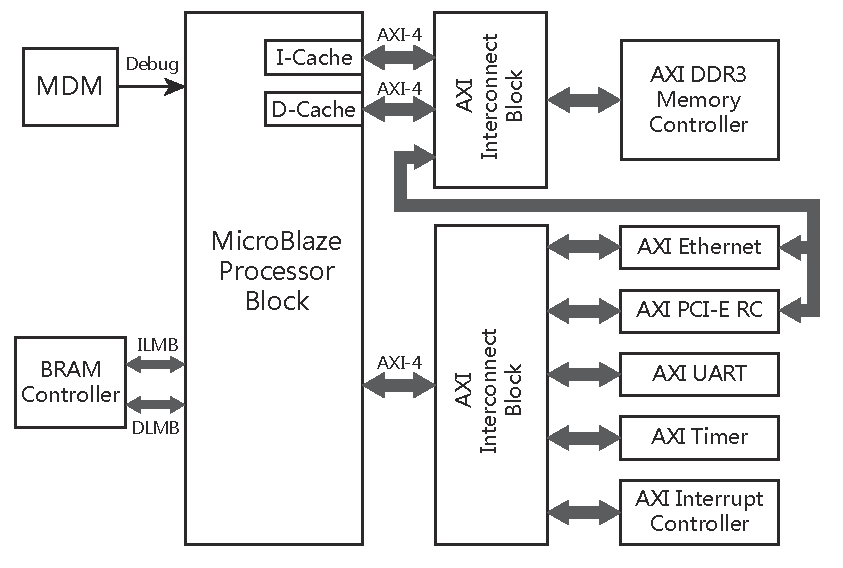
\includegraphics[width=0.6\textwidth]{impl/microblaze-base-arch}
  \caption{MicroBlaze基础架构}
  \label{fig:microblaze-base-arch}
\end{figure}


基于MicroBlaze的一个典型系统架构如图\ref{fig:microblaze-base-arch}所示,
MicroBlaze系统的固件代码保存在Block Memory中,
通过LMB(Local Memory Bus)总线连接到处理器核;
缓存子系统采用哈佛结构,具有分离的指令与数据缓存,它们通过AXI4总线连接到内存控制器;
I/O子系统同样使用AXI4总线互连,其中包括基本的外设,如中断控制器、串口、时钟等,
也支持一些复杂的I/O设备,如以太网\cite{axi-ethernet-subsystem}、
PCI-E\cite{axi-pcie-bridge}等。
MicroBlaze同时还提供了硬件调试接口,可以通过JTAG对其进行调试。

目前Xilinx提供的MicroBlaze软核并不支持多处理器架构,
在硬件实现上没有提供处理器间同步、通信机制,
之前一些工作\cite{microblaze-mp-rsp08,microblaze-mp-xapp}尝试为其增加多处理器支持,
但这些工作只是实现也最底层的处理器间同步、通信机制,
没有可用的操作系统层次上的多核支持。
受到该因素的影响,本文所设计的PARD原型系统只实现了``伪多核''的系统,
即系统中存在多个处理器核,但每个一逻辑域都被限制为只能使用一个处理器核。
未来MicroBlaze的多核软硬件支持完善后,可以很容易的将PARD原型系统的这一限制解除,
实现真正的多核系统。


\subsection{PARD原型系统架构}

PARD原型系统架构如图\ref{fig:pard-arch-impl}所示,
该系统由处理器子系统、I/O子系统、PRM SoC三部分组成。
其中处理器子系统包含四个处理器核心、共享缓存和内存控制器;
I/O子系统中包含四个串口控制器、两个以太网控制器和一个PCI Express根逻辑(RootComplex),
系统中所有的数据通路使用AXI4总线连接;
PRM同样是基于MicroBlaze的SoC系统,对外提供串口与SFP以太网接口,
同时通过内部串口与I/O子系统相连,用于接收I/O子系统的串口输出,
使用I2C总线作为控制平面网络的数据链路层,连接到系统中的四个控制平面:
处理器核控制平面CoreCP、共享缓存控制平面CacheCP、内存控制器控制平面MemCP和
I/O子系统控制平面I/OCP。

\begin{figure}[tb]
  \centering
  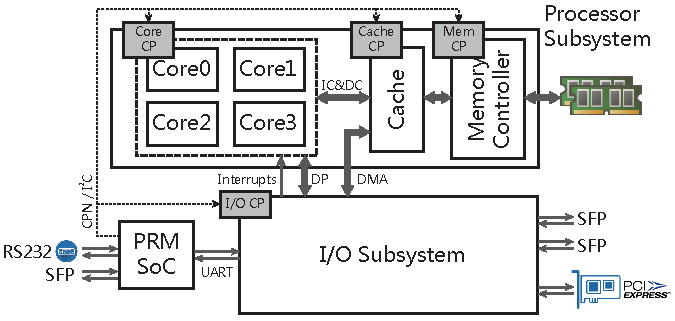
\includegraphics[width=0.8\textwidth]{impl/pard-arch-impl}
  \caption{PARD原型系统架构}
  \label{fig:pard-arch-impl}
\end{figure}

% 如何增加标签寄存器
处理器核心使用MicroBlaze软核及其他附属模块组成,
其内部结构如图\ref{fig:pard-core-impl}所示,
其中包含MicroBlaze软核、中断控制器和时钟模块,
该模块从外部输入时钟、复位和中断信号,
通过三个AXI4接口(IC指令缓存端口、DC数据缓存端口和DP外设端口)与外部交换数据。
AXI4总线协议中使用独立的通道实现读写请求、数据与响应,
其中读写请求中包含用户自定义信号,本文使用该信号在系统中传播应用标签。
由于MicroBlaze并没有开放源代码,处理器核的请求标记工作需要在核外进行:
首先在核外增加了一个标签寄存器,CoreCP连接到该寄存器,并可以对其内容进行修改;
在IC/DC/DP三个端口外分别增加三个标签模块,
用于将标签寄存器的值附加到AXI4总线AR/AW两个通道的USER信号中,完成请求标记。

% 增加共享缓存模块:支持16路、实现标签传播、实现划分
Xilinx为AXI4总线提供了一个缓存功能的IP核SystemCache\cite{pg118-system-cache},
其默认配置最多只能够支持4路组关联,这对于四核的PARD原型系统来说,
不足以验证缓存容量划分的功能,本文通过修改IP核实现,将其扩展到16路组关联;
按照第\ref{chap:labeladdrspace:propagation}节所述的方式,为该模块增加了标签传播功能;
同时修改其默认LRU替换策略,使其支持按路划分功能,
并通过CacheCP对共享缓存的行为进行控制(参见第\ref{chap:impl:cachecp}节)。
% 实现的多核
该Cache模块提供MicroBlaze专用接口连接四个处理器核,
同时还提供了通用AXI Master接口连接I/O子系统的DMA通道。
内存控制器控制平面提供了地址映射功能,实现四个处理器核的内存资源划分,
第\ref{chap:impl:migcp}节将详细讨论内存控制器控制平面的实现。

% I/O子系统结构
PARD的I/O子系统内部结构如图\ref{fig:pard-io-impl}所示,
处理器子系统的DP端口经过I/O子系统控制平面的地址映射后,使用AXI总线连接到所有的硬件模块,
其中PCI-E和以太网模块中包含DMA功能,
因此按照第\ref{chap:labeladdrspace:tagging}节中所描述的方法在其中增加标签寄存器,
其DMA访存请求结构标记后通过AXI总线发送到Cache模块。
所有设备的中断信号在内部进行编码,经过I/O控制平面进行重映射处理后,发送给对应的处理器核。
I/O子系统控制平面的设计将在第\ref{chap:impl:iocp}节进行讨论。

\begin{figure}[b]
\begin{minipage}{0.48\textwidth}
  \centering
  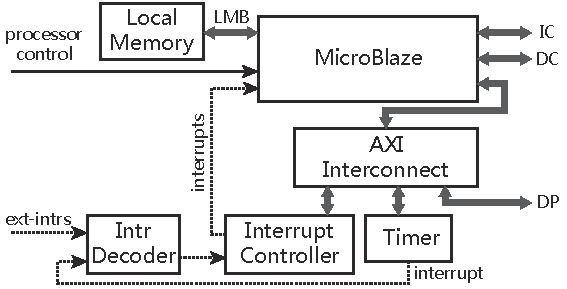
\includegraphics[width=\textwidth]{impl/pard-core-impl}
  \caption{PARD原型系统处理器核}
  \label{fig:pard-core-impl}
\end{minipage}\hfill
\begin{minipage}{0.48\textwidth}
  \centering
  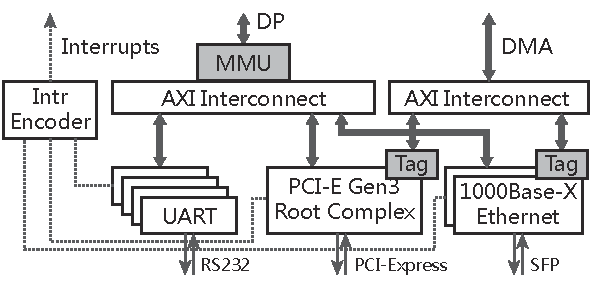
\includegraphics[width=\textwidth]{impl/pard-io-impl}
  \caption{PARD原型系统I/O子系统}
  \label{fig:pard-io-impl}
\end{minipage}
\end{figure}

% 原型的照片
本文使用Xilinx Virtex-7 FPGA(型号xc7vx690tffg1761-2)
在VC709平台上实现了上述PARD原型系统,如图\ref{fig:pard-fpga-board}所示。
该原型系统对外呈现三类接口:一个RS232串口,与PRM的串口相连;
三个SFP接口,其中两个连接到I/O子系统,另外一个与PRM的以太网接口相连;
一个PCI-E Gen3 x4接口,连接到I/O子系统,可以连接兼容的PCI-E设备,
在本例中在该接口连接了一块Intel PCI-E以太网卡(芯片型号82575)。

\begin{figure}[tb]
  \centering
  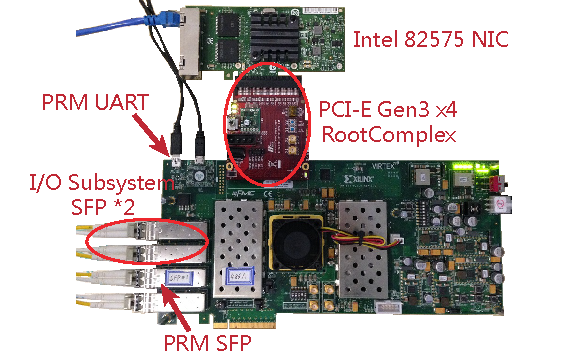
\includegraphics[width=0.6\textwidth]{impl/pard-fpga-board}
  \caption{PARD原型系统}
  \label{fig:pard-fpga-board}
\end{figure}

% 资源占用与FPGA布线结果
该原型系统在FPGA上的布局布线结果如图\ref{fig:pard-fpga-routed}所示。

% TODO: 增加资源使用情况,以及分模块的资源占用情况


\subsection{PRM与软件栈实现}

为何选择I2C,有何替代

如何改造I2C成为双向网络

连接多个控制平台

触发表中断传播机制
在第\ref{chap:impl:trigger-latency}节中将对触发表响应时间进行分析。


LDom的内核、rootfs和device-tree(完整的)


\section{控制平面实现}

\subsection{通用控制平面}

\subsubsection*{表设计}
\subsubsection*{状态表更新逻辑}
\subsubsection*{触发表逻辑}


\subsection{处理器核控制平面}
\label{chap:impl:corecp}

\subsection{共享末级缓存控制平面}
\label{chap:impl:cachecp}


\textbf{延迟分析}\quad
We find that the LLC control plane does not introduce
extra latency. According to Figure 4, the processing logic of the
LLC control plane can be hidden into the pipeline of the LLC
controller. In fact, pipelining is a typical design for modern CPUs’
LLC. For example, the L2 cache of OpenSPARC T1 has eight
pipeline stages, our Xilinx Cache has five stage pipeline.
Furthermore, synthesis data verify that the logic
of the LLC control plane is not in critical pathes.


\subsection{内存控制器控制平面}
\label{chap:impl:migcp}

\textbf{延迟分析}\quad
为实现内存控制器平面地址映射功能,在数据通路的关键路径上增加了额外的MMU模块,
但该模块并不会造成额外的延迟开销。
图\ref{fig:pard-cp-mmu-sim}是对MMU模块的仿真,可以看到每次访存的周期并没有发生变化。


\subsection{I/O子系统控制平面}
\label{chap:impl:iocp}

I/O子系统控制平面主要处理三个事件:
DP口请求地址重映射、
DMA口请求打标签、
中断重映射。

DP口请求地址重映射与内存控制器控制平面的实现相同,不同的是映射地址的范围,
在当前的I/O子系统实现中,其物理地址范围分配如表\ref{tab:pard-io-phyaddr}所示。

\begin{table}[htb]
  \centering
  \begin{minipage}[t]{0.8\linewidth}
  \caption{I/O子系统物理地址空间分配}
  \label{tab:pard-io-phyaddr}
    \begin{tabular*}{\linewidth}{cll}
      \toprule[1.5pt]
      \textbf{地址范围} & \textbf{硬件} & \textbf{用途} \\
      \midrule[1pt]
      \textit{0x48000000 - 0x4800FFFF} & Ethernet \#0       & 控制寄存器    \\
      \textit{0x48100000 - 0x4810FFFF} & Ethernet DMA \#0   & DMA控制寄存器 \\
      \textit{0x48200000 - 0x4820FFFF} & Ethernet \#1       & 控制寄存器    \\
      \textit{0x48300000 - 0x4830FFFF} & Ethernet DMA \#1   & DMA控制寄存器 \\
      \textit{0x60000000 - 0x6FFFFFFF} & PCI-E Root Complex & 控制寄存器    \\
      \textit{0x70000000 - 0x7FFFFFFF} & PCI-E Root Complex & PCI-E地址空间 \\
      \bottomrule[1.5pt]
    \end{tabular*}\\[2pt]
  \end{minipage}
\end{table}

控制平面中记录了每个设备被哪个逻辑域使用,其中包括地址范围映射信息和中断映射信息,
通过中断路由模块将中断发送到对应的处理器核。


\section{数据平面实现}

我们修改了该原型系统的内存控制器部分,在其中增加了数据平面处理器(图10箭头所标识的区域),通过软件代码的方式实现内存地址映射功能。为简化实现,我们使用精简配置的MicroBlaze实现数据平面处理器的功能。

(1)将MicroBlaze配置为精简模式,去除所有与数据平面处理器无关的可选指令,如:硬件FPU、乘法器/除法器、扩展指令等;关闭MMU、Cache、中断异常等高级功能,只保留最基本的算术逻辑部分。通过精简配置,MicroBlaze系统的频率从133MHz提高到了250MHz。

(2)使用MicroBlaze提供的Stream Link接口作为数据平面处理器的请求接口。由于目前MicroBlaze的Stream Link接口是固定的32位AXIS接口,我们将多个Stream Link合并使用作为一个请求接口。

(3)MicroBlaze提供put/get指令实现对Stream Link的接口,通过合并多个put或get指令即可实现请求缓存指令rbput和rbget。如表\ref{tab:pard-dp-isa-impl}所示,``请求''类型的长度为12个字节,我们使用3个MicroBlaze通用寄存器(r10-r12)作为请求寄存器,通过使用get/put指令操作Stream Link接口fsl0,实现rbget和rbput的功能。

\begin{table}[htb]
  \centering
  \begin{minipage}[t]{0.6\linewidth}
  \caption{请求缓存指令的MicroBlaze实现}
  \label{tab:pard-dp-isa-impl}
    \begin{tabular*}{\linewidth}{lp{0.5cm}lp{0.5cm}l}
      \toprule[1.5pt]
       & \multicolumn{2}{l}{\textbf{rbput}} & \multicolumn{2}{l}{\textbf{rbget}} \\ 
      \midrule[1pt]

      \multirow{8}{2cm}{\textbf{MicroBlaze指令实现}} & \multicolumn{2}{l}{rbput:}   & \multicolumn{2}{l}{rbget:} \\
                                                   &  & nget fsl0                 &  & nput fsl0               \\
                                                   &  & addc r3, r0, r0           &  & addc r3, r0, r0         \\
                                                   &  & bneq ret                  &  & bneq ret                \\
                                                   &  & get r10, fsl0             &  & put r10, fsl0           \\
                                                   &  & get r11, fsl1             &  & put r11, fsl1           \\
                                                   &  & get r12, fsg2             &  & put r12, fsl2           \\
                                                   & \multicolumn{2}{l}{ret:}     & \multicolumn{2}{l}{ret:}   \\
      \bottomrule[1.5pt]
    \end{tabular*}\\[2pt]
  \end{minipage}
\end{table}


\section{性能评估}

前三节使用microbenchmark:stream测带宽、spec测ipc

由于MicroBlaze的TLB中没有类似AccessBit的访问历史信息,
在当前的linux kernel实现中TLB替换策略使用的是clock算法,
这造成应用在运行过程中频繁发生TLB miss与重填动作,
大约有一半以上的时间花费在kernel中执行TLB相关操作,
造成corecp和cachecp统计的IPC与命中率不准确。
为了得到准确的IPC与命中率信息,
我们将部分应用(429.mcf、cacheflush microbenchmark)移植到uboot环境下,
由于在uboot环境中由于并没有开启MMU,因此不会受到TLB的影响。
而像memcached这样的应用,对操作系统的依赖很大,无法移植,
但这样的应用我们只关注其端到端的性能,因此这些性能上的差异可以忽略。


\subsection{区分化服务}

在PARD中使用逻辑域的抽象,可以为不同的逻辑域分配不同的资源,
本节将测试PARD如何为相同的应用分配不同的资源,以实现区分化服务的功能。
在本节的测试中将同时运行两个逻辑域,其配置完全相同,都包含一个处理器核和1GB的内存,
在其中运行相同的应用,通过cacehcp调整其缓存容量的分配,实现区分化服务。

\textbf{TODO: stream在不同cache容量下的表现}


图\ref{fig:diffserv-mcf-ipc-hitrate}给出了mcf的测试结果,在本实验中两个逻辑域分别分配了4路和12路的缓存容量,
从总执行时间上可以看到两者存在明显的差别,

\begin{figure}[tb]
  \centering
  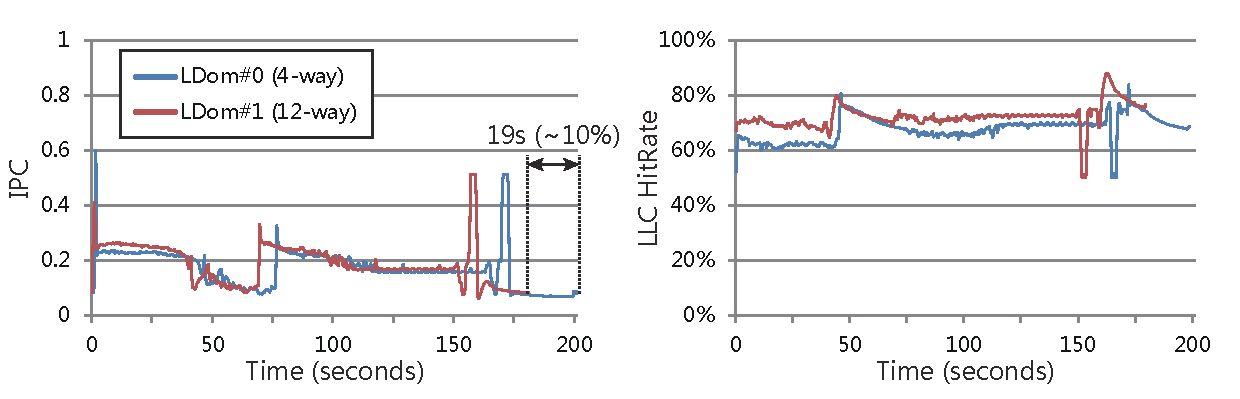
\includegraphics[width=\textwidth]{impl/diffserv-mcf-ipc-hitrate}
  \caption{区分化服务:429.mcf}
  \label{fig:diffserv-mcf-ipc-hitrate}
\end{figure}


\textbf{TODO: memcached在不同Cache容量下的表现}

为了评估在内存控制器控制平面提供的区分化服务功能,在本实验中关闭了Cache模块,
让处理器的访存请求直接发送到内存控制器。
使用stream测试单个逻辑域的访存带宽为19.8MB/s,以此作为对比的基线。
在测试过程中,我们发现内存控制器的性能要远高于四个MicroBlaze处理器同时访存的需求,
为了进行本实验,需要对原型系统进行修改,使内存控制器发生资源竞争,
具体做法如下:将第四个处理器核更换为一个访存负载发生器,由它持续向内存控制器发送访存请求,
为了保证系统正确运行,该负载发生器只生成读请求,其余三个处理器核分别运行逻辑域,
并在其中使用stream发送读请求测试访存带宽。
在内存控制器控制平面为这三个逻辑域设置不同的优先级,同时为负载发生器设置为低优先级。
图\ref{fig:diffserv-stream-generator}给出了评测结果,
可以看到三个逻辑域的访存性能有明显的区分,相比于基线分别有89\%、52\%和36\%的带宽下降,
而负载发生器本身的访存带宽也从268MB/s下降到100MB/s。
目前内存控制器调度策略只实现了三个优先级,无法对每个逻辑域带宽进行精确控制,
后续可以对策略进行修改,以实现基于目标带宽的调度策略。

\begin{figure}[htb]
  \centering
  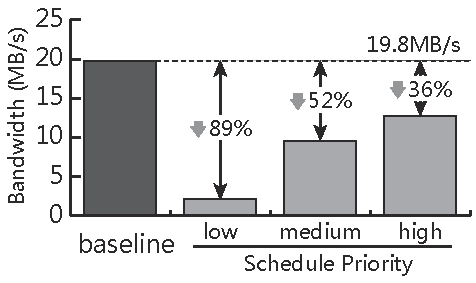
\includegraphics[width=0.5\textwidth]{impl/diffserv-stream-generator}
  \caption{区分化服务:访存优先级}
  \label{fig:diffserv-stream-generator}
\end{figure}

\subsection{性能隔离}

一个LDom运行关键应用(如mcf或stream),另外三个LDom进行干扰,
 - 通过cache划分,实现性能隔离;
 - 在mig前增加干扰,保证关键应用性能不受影响

图\ref{fig:isolation-mcf-ipc-hitrate}给了隔离测试结果,LDom\#0运行mcf,
另外三个逻辑域运行干扰应用,单独运行时独占所有16路的Cache,执行时间大约为150秒;
与三个干扰应用同时运行时,执行时间延长到222秒,大约增加了48\%;
使用隔离的方式,将12路Cache分配给mcf,性能恢复,只增加了7\%的执行时间。

\begin{figure}[tb]
  \centering
  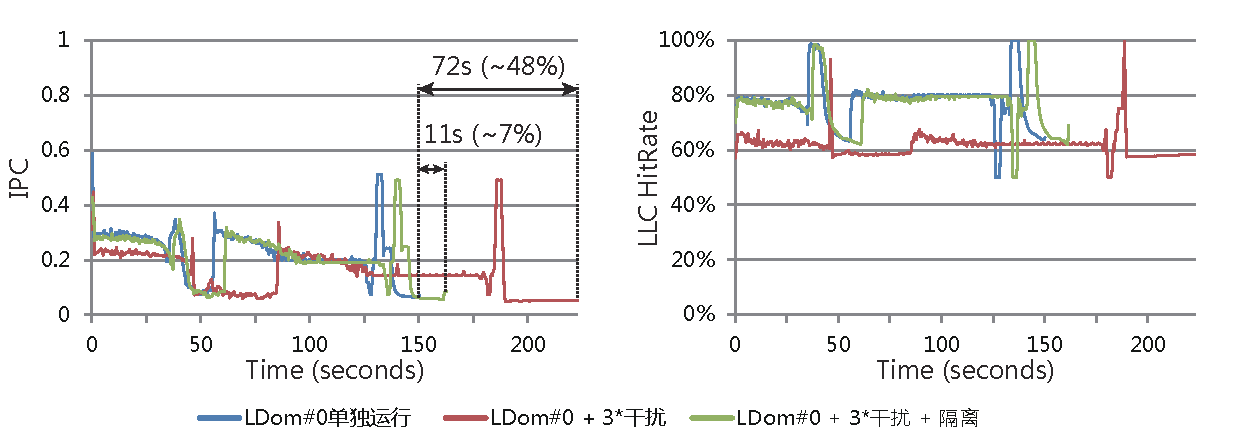
\includegraphics[width=\textwidth]{impl/isolation-mcf-ipc-hitrate}
  \caption{性能隔离:429.mcf}
  \label{fig:isolation-mcf-ipc-hitrate}
\end{figure}


\subsection{策略生效时间}
\label{chap:impl:trigger-latency}

一个LDom运行mcf,另外三个运行干扰;
写一个trigger=>action,通过ipc/missrate控制waymask,
测试生效时间:
 - 应用性能变化 (理论上没有变化)
 - 总的响应时间 + 响应时间分段
 - 结论:没有实现ms级的原因是microblaze性能问题

在PARD体系结构基于表的控制平面设计中,
``Trigger$\Rightarrow$Action''机制的反馈时间可以主要分为Trigger事件检测、
控制平面网络传送事件消息、PRM处理事件、以及控制平面网络传送Action的参数修改四个部分。
其中第一阶段由控制表硬件逻辑完成,可以在有限的时钟周期内完成;
第二和第四阶段由于需要使用控制平面网络传送数据,因此其响应时间与控制平面网络的速率相关,
在我们目前的原型系统中,由于使用了I2C总线作为控制平面网络,其最高速率为1Mbit/s,
对于一个32bit的事件消息以及一组96bit的参数修改消息,至少需要128us完成数据传输,
如果需要传输更多的消息则需要消耗更长的时间;
第三阶段PRM处理中,需要经过控制平面驱动、内核、用户态三个层次进行处理,也需要消耗一定的时间。
在采用可编程数据平面架构后,对Trigger事件的反馈调节代码可以直接在数据平面的固件代码中完成,
消除了PARD原有设计中需要经过PRM进行统一处理的时间消耗,实现更快速的反馈响应。

但数据平面处理器的引入也给性能造成影响,第\ref{chap:impl:dp-latency}节将对性能数据平面处理器的性能进行分析。


%\subsection{实际应用测试}
%
%使用memcached测试,加入trigger=>action机制,得出与模拟器相同的结果

\subsection{数据平面处理器延迟分析}
\label{chap:impl:dp-latency}

%通过使用可编程处理器来替代硬件逻辑,可以极大增强设备的可编程能力,
%但由于处理器位于硬件请求处理的关键路径,我们需要对其性能与资源开销进行评估,
%以确保其不会对系统性能与开销造成严重的影响。
%本章以内存控制器的可编程数据平面为例,对其可编程数据平面的资源开销进行分析;
%并通过stream与memcached两种应用负载来评估其对系统性能的影响;
%最后我们分析了可编程数据平面架构对PARD体系结构中``Trigger=>Action''机制反馈时间的优化。

与硬件逻辑实现相比,可编程处理器在系统中引入了额外的开销,
我们通过内存控制器上增加本文所提出的可编程数据平面架构,
实现与PARD中相同的地址映射功能,来验证该架构对系统延迟的影响。

系统延迟的大小与应用和固件功能相关,因此我们选择与硬件实现完全相同的地址映射功能,
并使用内存带宽测试工具stream和内存键值存储应用memcached对系统的延迟进行评估。
由于受到FPGA设备的限制,在我们的平台下MicroBlaze软核处理器最高只能工作在250MHz的频率,
我们选择了100MHz/150MHz/200MHz/250MHz四种不同的频率对系统延迟进行了评估。

\textbf{访存带宽}\quad
在PARD的控制平面设计中,实现地址映射的控制表并没有引入额外的延迟开销,
其性能与直接访问内存控制器相同,受到MicroBlaze处理器性能的限制,
我们在能够得到25.1MB/s的访存带宽(如图\ref{fig:pard-dp-stream}所示)。

由于地址映射功能只需要对请求地址进行操作,而无需对数据进行修改,
因此我们实现了一个简化版本的数据平面处理器(工作在100MHz频率),
该处理器只对地址请求进行处理,数据绕过处理器直接发送到内存控制器。
在使用该设计后测得的访存带宽是21.5MB/s,与非处理器实现相比并没有特别明显的下降。

为了使数据平面处理器对访存数据也能够进行操作,我们将数据请求也发送到处理器进行处理,
在100MHz频率下测得的访存带宽出现了明显的下降,只有13MB/s。
进一步提高数据平面处理器的工作频率,带宽基本呈现线性上升,
在150MHz时能够得到15MB/s的访存带宽;
在200MHz时,访存带宽提高到了20MB/s;
而在250MHz时,访存带宽达到了22.5MB/s。
由于受到FPGA硬件的限制,我们无法实现更高频率的数据平面处理器,
但数据平面处理器的功能十分精简,如果使用ASIC工艺,可以得到更高的频率,
因此其处理器的性能不会成为系统的瓶颈。

\textbf{memcached性能}\quad
访存带宽只能作为系统性能的一个评估指标,系统运行时的实际开销要与应用相关联。
图\ref{fig:pard-dp-memcached}给出了memcached在同硬件配置下的性能变化,
与访存带宽的结果类似,memcached的性能与数据平面处理器频率相关,
当工作在100MHz频率时,只能得到568RPS的性能,
但如果处理器频率提升到250MHz,其性能(618RPS)与使用控制表的方案(628RPS)基本接近。

\begin{figure}[tb]
\begin{minipage}{0.48\textwidth}
  \centering
  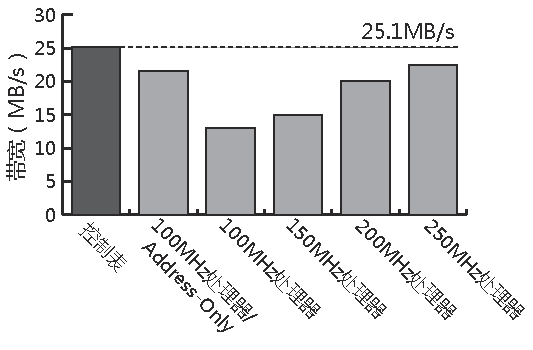
\includegraphics[width=\textwidth]{impl/pard-dp-stream}
  \caption{访存带宽对比}
  \label{fig:pard-dp-stream}
\end{minipage}\hfill
\begin{minipage}{0.48\textwidth}
  \centering
  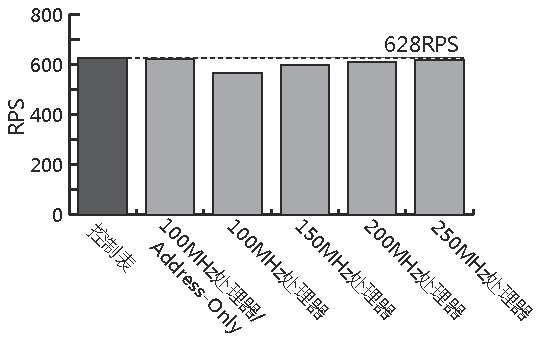
\includegraphics[width=\textwidth]{impl/pard-dp-memcached}
  \caption{memcached性能对比}
  \label{fig:pard-dp-memcached}
\end{minipage}
\end{figure}


\section{资源开销评估}

PARD的资源开销主要体现在三个方面,分别是:
用于标签传播的资源开销、
控制平面的资源开销、
数据平面的资源开销。
本节将分别对这三方面的开销进行评估。

\subsection{标签传播资源开销}

\subsection{控制平面资源开销}

控制平面的资源开销主要体系在表存储、触发逻辑两方面,
使用CAM结构,因此需要消耗大量的LUT和FF资源。具体如表\ref{tab:pard-cp-resource}所示。


\subsection{数据平面资源开销}

可编程数据平面的资源开销主要在处理器逻辑及其使用的scratchpad memory两个方面。
在通过配置精简后,MicroBlaze处理器所占用的资源量大大减少,
其Slice(LUT和FF)占用只有完整配置的50\%左右,
scratchpad memory的容量由固件代码的大小决定,
当前的实现中我们为其保留了32KB的容量,在FPGA中占用了8个RAMB36资源。
原型系统中主要的硬件部件与可编程数据平面占用的FPGA资源如表\ref{tab:pard-dp-resource}所示。
可以看到可编程数据平面在只占用有限的FPGA资源下,为硬件增加了更为灵活的可编程能力。

\begin{table}[htb]
  \centering
  \begin{minipage}[t]{0.9\linewidth}
  \caption{数据平面处理器、共享缓存与内存控制器资源占用情况(xc7vx690t设备)}
  \label{tab:pard-dp-resource}
    \begin{tabular*}{\linewidth}{cccc}
      \toprule[1.5pt]
      \textbf{组件} & \textbf{Slice LUT} & \textbf{Slice Register} & \textbf{Block RAM(RAMB36)} \\
      \midrule[1pt]
      16-way/512KB共享缓存    &  7590       &  5664            &  161               \\
      内存控制器              &  13471      &  10562           &  1                 \\
      完整配置的MicroBlaze核  &  4896       &  8526            &  12                \\
      \hline
      数据平面处理器          &  1433       &  5524            &  8                 \\
      \bottomrule[1.5pt]
    \end{tabular*}\\[2pt]
  \end{minipage}
\end{table}


\section{小结}


\begin{figure}[htb]
  \centering
  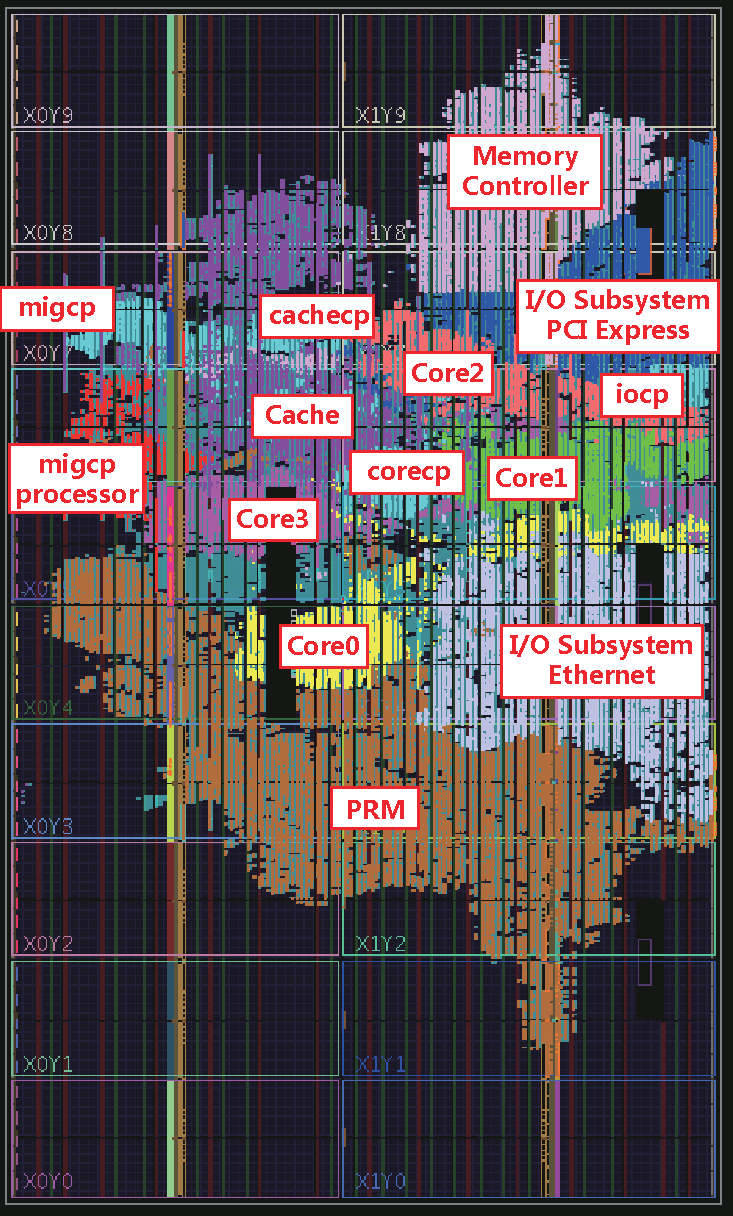
\includegraphics[width=0.8\textwidth]{impl/pard-fpga-routed}
  \caption{PARD原型系统布局布线结果}
  \label{fig:pard-fpga-routed}
\end{figure}


%%% Local Variables:
%%% mode: latex
%%% TeX-master: t
%%% End:

\chapter{结束语}
\label{cha:concl}

\section{本文工作总结}
This paper presented a study of building DiffServ in computer
servers via architectural support. We proposed programmable
architecture for resourcing-on-demand(PARD) and developed a
Linux-based firmware to facilitate programming PARD. We implemented
PARD on both a full-system simulator and an FPGA
development board. Our experiments demonstrated that PARD is
able to address the trade-offs between high utilization and high
QoS in datacenter environments.


\section{下一步研究方向}

We believe that architectural support for DiffServ in computers
is a promising trend as the number of cores keeps increasing. PARD
makes a case for this direction and provides new interfaces for users
to interact with the hardware. However, there are still a lot of open
issues such as

how to translate applications’ QoS requirements into efficient
“trigger)action” rules?

how to leverage compilers to automatically generate trigger
rules?

how to make OS directly run on PARD server to support
process-level DiffServ?

how to support fine-grain Diffserv for not only process-level but
also thread-level or even C++/Java object-level?

how to support nested DiffServ, i.e., guarantee QoS of a process
within a LDom?
 
how to deal with simultaneous multithreading (SMT)?
 
how to deal with multiple processors issues such as cache coherency?

how to extend DiffServ to accelerators, e.g., enabling an encryption
engine to encrypt/decrypt LDoms with specific DS-id?

how to integrate PARD and SDN so that DS-id can be propagated
in a data center wide?

how to design and deploy security policy on PARD servers?

how to develop firmware applications to take advantage of
PARD?

To facilitate further optimization and exploration, we
release the PARD-gem5 simulator that is available at
https://github.com/fsg-ict/PARD-gem5.



% 参考文献
%\bibliographystyle{GBT7714-2005NLang-UTF8}
\bibliographystyle{unsrt}
\bibliography{ref/pard_asplos,ref/latest,ref/soft_proc_core,ref/crad,ref/softpard}

% 附录
\begin{appendix}
%%%% Local Variables: 
%%% mode: latex
%%% TeX-master: "../main"
%%% End: 

\chapter{外文资料原文}
\label{cha:engorg}
As one of the most widely used techniques in operations research, {\em
  mathematical programming} is defined as a means of maximizing a quantity known
as {\em objective function}, subject to a set of constraints represented by
equations and inequalities. Some known subtopics of mathematical programming are
linear programming, nonlinear programming, multiobjective programming, goal
programming, dynamic programming, and multilevel programming$^{[1]}$.

It is impossible to cover in a single chapter every concept of mathematical
programming. This chapter introduces only the basic concepts and techniques of
mathematical programming such that readers gain an understanding of them
throughout the book$^{[2,3]}$.


\section{Single-Objective Programming}
The general form of single-objective programming (SOP) is written
as follows,
\begin{equation}\tag*{(123)} % 如果附录中的公式不想让它出现在公式索引中,那就请
                             % 用 \tag*{xxxx}
\left\{\begin{array}{l}
\max \,\,f(x)\\[0.1 cm]
\mbox{subject to:} \\ [0.1 cm]
\qquad g_j(x)\le 0,\quad j=1,2,\cdots,p
\end{array}\right.
\end{equation}
which maximizes a real-valued function $f$ of
$x=(x_1,x_2,\cdots,x_n)$ subject to a set of constraints.

\newtheorem{mpdef}{Definition}[chapter]
\begin{mpdef}
In SOP, we call $x$ a decision vector, and
$x_1,x_2,\cdots,x_n$ decision variables. The function
$f$ is called the objective function. The set
\begin{equation}\tag*{(456)} % 这里同理,其它不再一一指定。
S=\left\{x\in\Re^n\bigm|g_j(x)\le 0,\,j=1,2,\cdots,p\right\}
\end{equation}
is called the feasible set. An element $x$ in $S$ is called a
feasible solution.
\end{mpdef}

\newtheorem{mpdefop}[mpdef]{Definition}
\begin{mpdefop}
A feasible solution $x^*$ is called the optimal
solution of SOP if and only if
\begin{equation}
f(x^*)\ge f(x)
\end{equation}
for any feasible solution $x$.
\end{mpdefop}

One of the outstanding contributions to mathematical programming was known as
the Kuhn-Tucker conditions\ref{eq:ktc}. In order to introduce them, let us give
some definitions. An inequality constraint $g_j(x)\le 0$ is said to be active at
a point $x^*$ if $g_j(x^*)=0$. A point $x^*$ satisfying $g_j(x^*)\le 0$ is said
to be regular if the gradient vectors $\nabla g_j(x)$ of all active constraints
are linearly independent.

Let $x^*$ be a regular point of the constraints of SOP and assume that all the
functions $f(x)$ and $g_j(x),j=1,2,\cdots,p$ are differentiable. If $x^*$ is a
local optimal solution, then there exist Lagrange multipliers
$\lambda_j,j=1,2,\cdots,p$ such that the following Kuhn-Tucker conditions hold,
\begin{equation}
\label{eq:ktc}
\left\{\begin{array}{l}
    \nabla f(x^*)-\sum\limits_{j=1}^p\lambda_j\nabla g_j(x^*)=0\\[0.3cm]
    \lambda_jg_j(x^*)=0,\quad j=1,2,\cdots,p\\[0.2cm]
    \lambda_j\ge 0,\quad j=1,2,\cdots,p.
\end{array}\right.
\end{equation}
If all the functions $f(x)$ and $g_j(x),j=1,2,\cdots,p$ are convex and
differentiable, and the point $x^*$ satisfies the Kuhn-Tucker conditions
(\ref{eq:ktc}), then it has been proved that the point $x^*$ is a global optimal
solution of SOP.

\subsection{Linear Programming} 
\label{sec:lp}

If the functions $f(x),g_j(x),j=1,2,\cdots,p$ are all linear, then SOP is called
a {\em linear programming}.

The feasible set of linear is always convex. A point $x$ is called an extreme
point of convex set $S$ if $x\in S$ and $x$ cannot be expressed as a convex
combination of two points in $S$. It has been shown that the optimal solution to
linear programming corresponds to an extreme point of its feasible set provided
that the feasible set $S$ is bounded. This fact is the basis of the {\em simplex
  algorithm} which was developed by Dantzig as a very efficient method for
solving linear programming.
\begin{table}[ht]
\centering
  \centering
  \caption*{Table~1\hskip1em This is an example for manually numbered table, which
    would not appear in the list of tables}
  \label{tab:badtabular2}
  \begin{tabular}[c]{|c|m{0.8in}|c|c|c|c|c|}\hline
    \multicolumn{2}{|c|}{Network Topology} & \# of nodes & 
    \multicolumn{3}{c|}{\# of clients} & Server \\\hline
    GT-ITM & Waxman Transit-Stub & 600 &
    \multirow{2}{2em}{2\%}& 
    \multirow{2}{2em}{10\%}& 
    \multirow{2}{2em}{50\%}& 
    \multirow{2}{1.2in}{Max. Connectivity}\\\cline{1-3}
    \multicolumn{2}{|c|}{Inet-2.1} & 6000 & & & &\\\hline
    \multirow{2}{1in}{Xue} & Rui  & Ni &\multicolumn{4}{c|}{\multirow{2}*{\ucasthesis}}\\\cline{2-3}
    & \multicolumn{2}{c|}{ABCDEF} &\multicolumn{4}{c|}{} \\\hline
\end{tabular}  
\end{table}

Roughly speaking, the simplex algorithm examines only the extreme points of the
feasible set, rather than all feasible points. At first, the simplex algorithm
selects an extreme point as the initial point. The successive extreme point is
selected so as to improve the objective function value. The procedure is
repeated until no improvement in objective function value can be made. The last
extreme point is the optimal solution.

\subsection{Nonlinear Programming}

If at least one of the functions $f(x),g_j(x),j=1,2,\cdots,p$ is nonlinear, then
SOP is called a {\em nonlinear programming}.

A large number of classical optimization methods have been developed to treat
special-structural nonlinear programming based on the mathematical theory
concerned with analyzing the structure of problems.
\begin{figure}[h]
  \centering
  
\includegraphics[clip]{thu-lib-logo}
  \caption*{Figure~1\hskip1em This is an example for manually numbered figure,
    which would not appear in the list of figures}
  \label{tab:badfigure2}    
\end{figure}

Now we consider a nonlinear programming which is confronted solely with
maximizing a real-valued function with domain $\Re^n$.  Whether derivatives are
available or not, the usual strategy is first to select a point in $\Re^n$ which
is thought to be the most likely place where the maximum exists. If there is no
information available on which to base such a selection, a point is chosen at
random. From this first point an attempt is made to construct a sequence of
points, each of which yields an improved objective function value over its
predecessor. The next point to be added to the sequence is chosen by analyzing
the behavior of the function at the previous points. This construction continues
until some termination criterion is met. Methods based upon this strategy are
called {\em ascent methods}, which can be classified as {\em direct methods},
{\em gradient methods}, and {\em Hessian methods} according to the information
about the behavior of objective function $f$. Direct methods require only that
the function can be evaluated at each point. Gradient methods require the
evaluation of first derivatives of $f$. Hessian methods require the evaluation
of second derivatives. In fact, there is no superior method for all
problems. The efficiency of a method is very much dependent upon the objective
function.

\subsection{Integer Programming}

{\em Integer programming} is a special mathematical programming in which all of
the variables are assumed to be only integer values. When there are not only
integer variables but also conventional continuous variables, we call it {\em
  mixed integer programming}. If all the variables are assumed either 0 or 1,
then the problem is termed a {\em zero-one programming}. Although integer
programming can be solved by an {\em exhaustive enumeration} theoretically, it
is impractical to solve realistically sized integer programming problems. The
most successful algorithm so far found to solve integer programming is called
the {\em branch-and-bound enumeration} developed by Balas (1965) and Dakin
(1965). The other technique to integer programming is the {\em cutting plane
  method} developed by Gomory (1959).

\hfill\textit{Uncertain Programming\/}\quad(\textsl{BaoDing Liu, 2006.2})

\section*{References}
\noindent{\itshape NOTE: these references are only for demonstration, they are
  not real citations in the original text.}

\begin{enumerate}[{$[$}1{$]$}]
\item Donald E. Knuth. The \TeX book. Addison-Wesley, 1984. ISBN: 0-201-13448-9
\item Paul W. Abrahams, Karl Berry and Kathryn A. Hargreaves. \TeX\ for the
  Impatient. Addison-Wesley, 1990. ISBN: 0-201-51375-7
\item David Salomon. The advanced \TeX book.  New York : Springer, 1995. ISBN:0-387-94556-3
\end{enumerate}

\chapter{外文资料的调研阅读报告或书面翻译}
\section{单目标规划}
北冥有鱼,其名为鲲。鲲之大,不知其几千里也。化而为鸟,其名为鹏。鹏之背,不知其几
千里也。怒而飞,其翼若垂天之云。是鸟也,海运则将徙于南冥。南冥者,天池也。 
\begin{equation}\tag*{(123)}
 p(y|\mathbf{x}) = \frac{p(\mathbf{x},y)}{p(\mathbf{x})}=
\frac{p(\mathbf{x}|y)p(y)}{p(\mathbf{x})}
\end{equation}

吾生也有涯,而知也无涯。以有涯随无涯,殆已!已而为知者,殆而已矣!为善无近名,为
恶无近刑,缘督以为经,可以保身,可以全生,可以养亲,可以尽年。

\subsection{线性规划}
庖丁为文惠君解牛,手之所触,肩之所倚,足之所履,膝之所倚,砉然响然,奏刀騞然,莫
不中音,合于桑林之舞,乃中经首之会。
\begin{table}[ht]
\centering
  \centering
  \caption*{表~1\hskip1em 这是手动编号但不出现在索引中的一个表格例子}
  \label{tab:badtabular3}
  \begin{tabular}[c]{|c|m{0.8in}|c|c|c|c|c|}\hline
    \multicolumn{2}{|c|}{Network Topology} & \# of nodes & 
    \multicolumn{3}{c|}{\# of clients} & Server \\\hline
    GT-ITM & Waxman Transit-Stub & 600 &
    \multirow{2}{2em}{2\%}& 
    \multirow{2}{2em}{10\%}& 
    \multirow{2}{2em}{50\%}& 
    \multirow{2}{1.2in}{Max. Connectivity}\\\cline{1-3}
    \multicolumn{2}{|c|}{Inet-2.1} & 6000 & & & &\\\hline
    \multirow{2}{1in}{Xue} & Rui  & Ni &\multicolumn{4}{c|}{\multirow{2}*{\ucasthesis}}\\\cline{2-3}
    & \multicolumn{2}{c|}{ABCDEF} &\multicolumn{4}{c|}{} \\\hline
\end{tabular}  
\end{table}

文惠君曰:“嘻,善哉!技盖至此乎?”庖丁释刀对曰:“臣之所好者道也,进乎技矣。始臣之
解牛之时,所见无非全牛者;三年之后,未尝见全牛也;方今之时,臣以神遇而不以目视,
官知止而神欲行。依乎天理,批大郤,导大窾,因其固然。技经肯綮之未尝,而况大坬乎!
良庖岁更刀,割也;族庖月更刀,折也;今臣之刀十九年矣,所解数千牛矣,而刀刃若新发
于硎。彼节者有间而刀刃者无厚,以无厚入有间,恢恢乎其于游刃必有余地矣。是以十九年
而刀刃若新发于硎。虽然,每至于族,吾见其难为,怵然为戒,视为止,行为迟,动刀甚微,
謋然已解,如土委地。提刀而立,为之而四顾,为之踌躇满志,善刀而藏之。”

文惠君曰:“善哉!吾闻庖丁之言,得养生焉。”


\subsection{非线性规划}
孔子与柳下季为友,柳下季之弟名曰盗跖。盗跖从卒九千人,横行天下,侵暴诸侯。穴室枢
户,驱人牛马,取人妇女。贪得忘亲,不顾父母兄弟,不祭先祖。所过之邑,大国守城,小
国入保,万民苦之。孔子谓柳下季曰:“夫为人父者,必能诏其子;为人兄者,必能教其弟。
若父不能诏其子,兄不能教其弟,则无贵父子兄弟之亲矣。今先生,世之才士也,弟为盗
跖,为天下害,而弗能教也,丘窃为先生羞之。丘请为先生往说之。”
\begin{figure}[h]
  \centering
  
\includegraphics{hello}
  \caption*{图~1\hskip1em 这是手动编号但不出现索引中的图片的例子}
  \label{tab:badfigure3}    
\end{figure}

柳下季曰:“先生言为人父者必能诏其子,为人兄者必能教其弟,若子不听父之诏,弟不受
兄之教,虽今先生之辩,将奈之何哉?且跖之为人也,心如涌泉,意如飘风,强足以距敌,
辩足以饰非。顺其心则喜,逆其心则怒,易辱人以言。先生必无往。”

孔子不听,颜回为驭,子贡为右,往见盗跖。

\subsection{整数规划}
盗跖乃方休卒徒大山之阳,脍人肝而餔之。孔子下车而前,见谒者曰:“鲁人孔丘,闻将军
高义,敬再拜谒者。”谒者入通。盗跖闻之大怒,目如明星,发上指冠,曰:“此夫鲁国之
巧伪人孔丘非邪?为我告之:尔作言造语,妄称文、武,冠枝木之冠,带死牛之胁,多辞缪
说,不耕而食,不织而衣,摇唇鼓舌,擅生是非,以迷天下之主,使天下学士不反其本,妄
作孝弟,而侥幸于封侯富贵者也。子之罪大极重,疾走归!不然,我将以子肝益昼餔之膳。”


\chapter{其它附录}
前面两个附录主要是给本科生做例子。其它附录的内容可以放到这里,当然如果你愿意,可
以把这部分也放到独立的文件中,然后将其 \verb|\input| 到主文件中。

\end{appendix}

%%% 其他部分
\backmatter

% 致谢
%%% Local Variables:
%%% mode: latex
%%% TeX-master: "../main"
%%% End:

\begin{ack}

转瞬在计算所读博的七年即将过去,这时才猛然发现,
和计算机相识已经16年了。
还记得初识时的CAI和LOGO,
还有那本似懂非懂的《数据结构:C语言描述》,
是我走上计算机道路的开始。
在这里要感谢那些给予我关怀、指导和帮助的人们。

首先要感谢我的导师孙凝晖老师,成为您的学生我的幸运。
您渊博的知识、严谨的治学态度和敏锐的思维,还有您对中国计算机事业的使命感,
是我今后学习的榜样。

还要感谢那些在重要的人生选择时给予我帮助的人:
感谢许强老师,是您将我从书本和实验带入到真正的项目,教会我需求分析、项目管理;
感谢董天正教授,是您带我进入到计算机系统结构领域;
感谢熊劲老师,您严谨的的治学态度,是我一直学习与坚持的榜样;
感谢李卓坚老师,是您手把手的教我认识机房与服务器,引领我进入系统管理的领域;
感谢马捷老师,您教会了我规范的重要。
特别要感谢包云岗老师,您是我的指路人,为我迷茫的博士路指明了方向,
也是在您的帮助下,我完成自己进入计算所时的梦想,造出了属于自己的计算机。

感谢计算所智能中心、高性能中心和先进计算机系统研究中心对我的培养。
感谢已经毕业的师兄们,
特别要感谢邢晶师兄、马灿师兄和李强师兄,是你们教会了我坚持与信念。
感谢与我共同奋斗的师弟师妹们:
感谢余子濠(濠神),我大PARD的重任就交给你了;
感谢黄博文、靳鑫,你们是我硬件入门的老师;
感谢展旭升、李宇鹏、徐天妮、姚治成、屈雨鹏、李文捷,和大家一起做科研是非常愉快的事情。
感谢张子刚,一起奋斗在博士的最后阶段,没有战友,一个人的战斗会非常的艰辛。

感谢徐志伟老师、冯晓兵老师、陈云霁老师、谢源老师、
孙广宇老师对我的学位论文提出了宝贵的修改意见。
感谢Donald E. Knuth以及Leslie Lamport,
他们开发的\TeX 和\LaTeX 使我可以专注于论文的写作。
还要感谢\ucasthesis 及其维护者xiaoyao9933,
它让我的论文写作轻松自在了许多,让我的论文格式规整漂亮了许多。

最后要感谢我的家人,感谢我的妈妈,
是您的关心与支持让我能够毫无顾虑的向着自己的理想奋斗,
您对我的爱是我一直前进的动力。

感谢我亲爱的妻子王一帆,一直默默的陪在我身边支持我、鼓励我,
是你的付出与理解,还有那些精心准备的爱心午餐,
让我能够专心科研、顺利毕业。

仅以此文,献给我的父亲。
\newline\newline

\rightline{2016年05月21日\qquad}
\rightline{于计算所\qquad\qquad}

\end{ack}


% 作者简介
\begin{resume}

\noindent
姓名:马久跃  性别:男  出生日期:1988.10.19  籍贯:辽宁\\

\noindent
2009.9 -- 现在       中国科学院计算技术所 计算机体系结构专业硕博研究生

\noindent
2005.9 -- 2009.7      东北师范大学软件学院 本科生\\

  \resumeitem{攻读博士学位期间发表的论文}
  \begin{enumerate}[leftmargin=1.5\parindent, nolistsep, label={[\arabic*]}]
    \item Jiuyue Ma, Xiufeng Sui, Ninghui Sun, Yupeng Li, Zihao Yu, Bowen Huang, Tianni Xu, Zhicheng Yao, Yu Chen, Haibin Wang, Lixin Zhang, Yungang Bao, Supporting Differentiated
    \item Jiuyue Ma, Xiufeng Sui, Yupeng Li, Zihao Yu, Bowen Huang, Yungang Bao, Supporting Differentiated Services in Datacenter Servers [C], OSDI'2014 Poster.
  \end{enumerate}

  \resumeitem{专利}
  \begin{enumerate}[leftmargin=1.5\parindent, nolistsep, label={[\arabic*]}]
    \item 马久跃,刘立坤,严得辰,李旭,基于设备能力的多终端数据同步方法和系统,申请号:201210208518.5,已授权
  \end{enumerate}

  \resumeitem{攻读博士学位期间参加的科研项目}
  \begin{enumerate}[leftmargin=1.5\parindent, nolistsep, label={[\arabic*]}]
    \item XX基金项目“共享存储机群系统的研究”(xxxxx),20xx年1月~20xx年12月
    \item 国家自然科学基金项目“共享存储机群系统中关键技术研究”(xxxxxxx),20xx年1月~20xx年12月
  \end{enumerate}

  \resumeitem{攻读博士学位期间的获奖情况}
  \begin{enumerate}[leftmargin=1.5\parindent, nolistsep, label={[\arabic*]}]
    \item 2011年被评为中国科学院``三好学生''
    \item 2012年获曙光博士奖学金
    \item 2015年获博士国家奖学金
  \end{enumerate}
\end{resume}


% 保证总页数为偶数。连续双面打印时,防止将两份论文的末页、首页打印在同一张纸上。
\cleardoublepage

\end{document}
